%%%%%%%%%%%%%%%%%%%%%%%%%%%%%%%%%%%%%%%%%%%%%%%%%%%%%%%%%%%%%%%%%%%%%%%%%%%%%%%%
% Template:
% Exam Notes LaTeX Template
% Version 1.0 (30/08/2018)
%
% Document:
% Signal Processing exam notes
%
% Original author:
% Rambod Rahmani <rambodrahmani@autistici.org>
%
% License: 
% Creative Commons Attribution-NonCommercial-ShareAlike 4.0 International
% License.
%%%%%%%%%%%%%%%%%%%%%%%%%%%%%%%%%%%%%%%%%%%%%%%%%%%%%%%%%%%%%%%%%%%%%%%%%%%%%%%%

%-------------------------------------------------------------------------------
% PACKAGES AND OTHER DOCUMENT CONFIGURATIONS
%-------------------------------------------------------------------------------

\documentclass[12pt,oneside,openany]{memoir}

\usepackage[utf8x]{inputenc}

\usepackage[T1]{fontenc}

\usepackage[italian]{babel}

\usepackage{url}

\usepackage{tabto}

\usepackage{wrapfig}

\usepackage[pdftex,dvipsnames]{xcolor}

\usepackage{gensymb}

\usepackage{amssymb,amsmath,amsthm}

\usepackage{mathtools}

\usepackage{mathpazo}

\usepackage{graphicx}

\usepackage{caption}

\usepackage{float}

\usepackage{csquotes}

\usepackage{afterpage}

\usepackage{hyperref}

\usepackage{textcomp}

\definecolor{mygreen}{RGB}{28,172,0}
\definecolor{mylilas}{RGB}{170,55,241}

\usepackage{listings}

\lstset{
	language=Matlab,
	basicstyle=\tiny,
	breaklines=true,
	morekeywords={matlab2tikz},
	keywordstyle=\color{blue},
	morekeywords=[2]{1}, keywordstyle=[2]{\color{black}},
	identifierstyle=\color{black},
	stringstyle=\color{mylilas},
	commentstyle=\color{mygreen},
	% without this there will be a symbol in the places where there is a
	% space
	showstringspaces=false,
	numbers=left,
	numberstyle={\tiny \color{black}},% size of the numbers
	numbersep=9pt, % this defines how far the numbers are from the text
	%some words to emphasise
	emph=[1]{for,end,break},emphstyle=[1]\color{red},
	%emph=[2]{word1,word2}, emphstyle=[2]{style},    
}

% Use more than one optional parameter in a new commands
\usepackage{xargs}

\usepackage[colorinlistoftodos,prependcaption,textsize=tiny]{todonotes}

\usepackage{expl3}
\ExplSyntaxOn
\cs_new_eq:NN \Repeat \prg_replicate:nn
\ExplSyntaxOff

\numberwithin{equation}{subsection}

% dedication environment
\newenvironment{dedication}
{
	% blank page before dedication
	\afterpage{\blankpage}
	% we want a new page
	\clearpage
	% no header and footer
	\thispagestyle{empty}
	% some space at the top 
	\vspace*{\stretch{1}}
	% the text is in italics
	\itshape
	% flush to the right margin
	\raggedleft
	% blank page after dedication
	\afterpage{\blankpage}
}
{
	% end the paragraph
	\par
	% space at bottom is one times that at the top
	\vspace{\stretch{1}}
	% finish off the page
	\clearpage
}

\newtheorem{theorem}{Teorema}[section]
\newtheorem{lemma}[theorem]{Lemma}

\DeclarePairedDelimiter{\abs}{\lvert}{\rvert}

\mathtoolsset{showmanualtags,mathic,centercolon}

\let\conjugate\overline

% blank page command
\newcommand{\blankpage}
{
    \null
    \thispagestyle{empty}%
    \addtocounter{page}{-1}%
    \newpage
}

\setcounter{chapter}{-1}

\epigraphfontsize{\small\itshape}
\setlength\epigraphwidth{8cm}
\setlength\epigraphrule{0pt}

% show subsection in the table of contents
\setcounter{tocdepth}{3}
\setcounter{secnumdepth}{3}

\newcommand{\quads}[1]{\Repeat{#1}{\quad}}
\newcommand{\dt}{\ dt}
\newcommand{\df}{\ df}

\newcommandx{\unsure}[2][1=]{\todo[linecolor=red,backgroundcolor=red!25,bordercolor=red,#1]{#2}}
\newcommandx{\change}[2][1=]{\todo[linecolor=blue,backgroundcolor=blue!25,bordercolor=blue,#1]{#2}}
\newcommandx{\info}[2][1=]{\todo[linecolor=OliveGreen,backgroundcolor=OliveGreen!25,bordercolor=OliveGreen,#1]{#2}}
\newcommandx{\improvement}[2][1=]{\todo[linecolor=Plum,backgroundcolor=Plum!25,bordercolor=Plum,#1]{#2}}
\newcommandx{\thiswillnotshow}[2][1=]{\todo[disable,#1]{#2}}

\epigraphfontsize{\small\itshape}

%-------------------------------------------------------------------------------
% TITLE PAGE
%-------------------------------------------------------------------------------

\title{%
	Esame Comunicazioni Numeriche\\
	\vspace{1cm}
	\large \textit{
		"What I hear, I forget;
		What I see, I remember;
		What I do, I understand."
	}}
\author{Rambod Rahmani}

\begin{document}
\renewcommand{\rmdefault}{cmr}

\maketitle
\pagenumbering{gobble}

\begin{dedication}
To my twin brother Ramtin.
\end{dedication}

%-------------------------------------------------------------------------------
% TABLE OF CONTENTS
%-------------------------------------------------------------------------------

\newpage
\pagenumbering{roman}
\tableofcontents
\afterpage{\blankpage}

\newpage
\pagenumbering{arabic}

%-------------------------------------------------------------------------------
% Chapter 0: Disclaimer
%-------------------------------------------------------------------------------

\chapter{Disclaimer}
\epigraph{"Information is power. But like all power, there are those who want
to keep it for themselves. The world's entire scientific and cultural heritage,
published over centuries in books and journals, is increasingly being digitized
and locked up by a handful of private corporations. There is no justice in
following unjust laws. It's time to come into the light and, in the grand
tradition of civil disobedience, declare our opposition to this private theft
of public culture."}{--- \textup{Aaron Swartz}}

The material and information in this document are provided "AS IS" in good faith
and without warranties of any kind, either expressed or implied.
\bigbreak\noindent
This work is licensed under:
\bigbreak\noindent
\href{http://creativecommons.org/licenses/by-nc-sa/4.0/}{
	
\includegraphics[height=\baselineskip]{images/cc_88x31.png} 
	Creative Commons Attribution-NonCommercial-ShareAlike 4.0 International 
	License}.

%-------------------------------------------------------------------------------
% Chapter 1: Introduction
%-------------------------------------------------------------------------------

\chapter{Introduction}
\epigraph{
	"The only person who is educated is the one who has learned how to
	learn and change."
}{--- \textup{Carl Rogers}}

This chapter contains introductory concepts needed as theoretical base to be
able to understand the signal processing topics presented in this text.

%-------------------------------------------------------------------------------
% Section 1: Complex Numbers
%-------------------------------------------------------------------------------

\section{Complex Numbers}
A complex number is a number that can be expressed in the form
\[z = a + ib,\]
where \(a\) is known to be the real part
\[a = \Re(z),\]
and \(b\) is known to be the imaginary part
\[b = \Im(z).\]
The complex number system can be defined as the algebraic extension of the
ordinary real numbers by an imaginary number \(i\). \(i\) is a solution of
the equation \(x^2 = −1\). Because no real number satisfies this equation, since
the square of a real number cannot be negative, \(i\) is called an imaginary
number.
\bigbreak
A real number \(a\) can be regarded as a complex number \(a + 0i\) whose
imaginary part is \(0\). A purely imaginary number \(bi\) is a complex number
\(0 + bi\) whose real part is zero. It is common to write \(a\) for \(a + 0i\)
and \(bi\) for \(0 + bi\).
\bigbreak
The complex numbers give rise to the fundamental theorem of algebra: every
non-constant polynomial equation with complex coefficients has a complex
solution. This property is true of the complex numbers, but not the reals. The
16th century Italian mathematician Gerolamo Cardano is credited with introducing
complex numbers in his attempts to find solutions to cubic equations.
\bigbreak
Geometrically, complex numbers extend the concept of the one-dimensional number
line to the two-dimensional complex plane by using the horizontal axis for the
real part and the vertical axis for the imaginary part.
\bigbreak
\textbf{Engineers reserve the letter \(i\) for electric current - the derivative
of electric charge with respect to time. We will therefore be using the letter
\(j\) instead of the letter \(i\).}

%-------------------------------------------------------------------------------
% Subsection 1: Cartesian form
%-------------------------------------------------------------------------------

\subsection{Cartesian form}
\begin{wrapfigure}{L}{0.5\textwidth}
	\centering
	\captionsetup{justification=centering}
	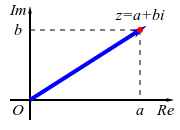
\includegraphics[width=0.5\textwidth]{images/complex_plane.png}
	\caption{A Complex Number in Cartesian Form.}
\end{wrapfigure}
A complex number can thus be identified with an ordered pair
\((\Re(z), \Im(z))\) in the Cartesian plane, an identification sometimes known
as the Cartesian form of \(z\). A complex number can be viewed as a point or
position vector in a two-dimensional Cartesian coordinate system called the
complex plane or Argand diagram, named after Jean-Robert Argand. The numbers are
conventionally plotted using the real part as the horizontal component, and
imaginary part as vertical (see Figure 1.1). In fact, a complex number can be
defined as an ordered pair \((a, b)\), but then rules for addition and
multiplication must also be included as part of the definition. William Rowan
Hamilton introduced this approach to define the complex number system.

%-------------------------------------------------------------------------------
% Subsection 2: Polar form
%-------------------------------------------------------------------------------

\subsection{Polar form}
\begin{wrapfigure}{L}{0.4\textwidth}
	\centering
	\captionsetup{justification=centering}
	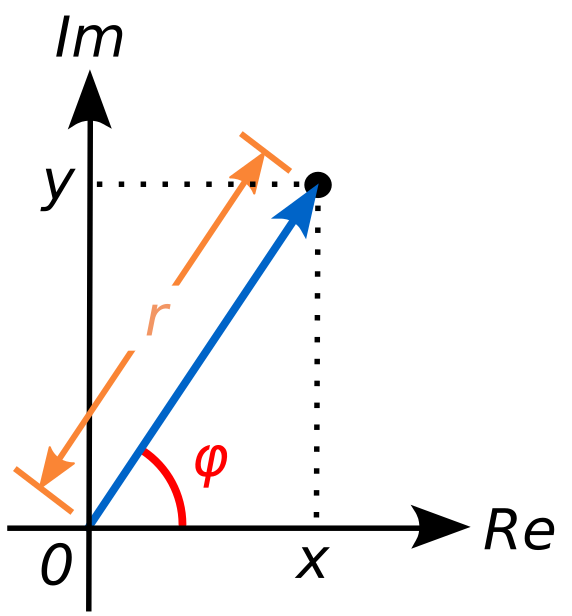
\includegraphics[width=0.4\textwidth]{images/complex_number_polar_form.png}
	\caption{A Complex Number in Polar Form}
\end{wrapfigure}
An alternative way of defining a point P in the complex plane, other than using
the \(a\)- and \(b\)-coordinates, is to use the distance of the point from \(O\)
, the point whose coordinates are \((0, 0)\) (the origin), together with the
angle subtended between the positive real axis and the line segment OP in a
counterclockwise direction. This idea leads to the polar form of complex numbers
. (see Figure 1.2 where \(x\) and \(y\) were used instead of \(a\) and \(b\)).
\bigbreak
The absolute value (or modulus or magnitude) of a complex number \(z = a + bj\)
is
\[c = \abs{z} = \sqrt{a^2 + b^2}\]
If \(z\) is a real number (that is, if \(b = 0\)), then \(c = \abs{a}\). That is
, the absolute value of a real number equals its absolute value as a complex
number. By Pythagoras' theorem, the absolute value of complex number is the
distance to the origin of the point representing the complex number in the
complex plane. 
\bigbreak
The argument of \(z\) (in many applications referred to as the "phase") is the
angle of the radius \(OP\) with the positive real axis, and is written as
\(arg(z)\). As with the modulus, the argument can be found from the rectangular
form \(a + bj\):
\[
	\varphi = arg(z) =
	\begin{cases}
		arctan\left(\frac{b}{a}\right) \quads{4} \ if \quad a > 0\\
		arctan\left(\frac{b}{a}\right) + \pi \quads{2} \ if \quad a < 0 
		\quad and \quad b \geq 0\\
		arctan\left(\frac{b}{a}\right) - \pi \quads{2} \ if \quad a < 0 
		\quad and \quad b < 0\\
		\frac{\pi}{2} \quads{8} if \quad a = 0 \quad and \quad b > 0\\
		-\frac{\pi}{2} \quads{7} if \quad a = 0 \quad and \quad b < 0\\
		indeterminate \quads{2} \ \ if \quad a > 0
	 \end{cases}
\]
The value of \(\varphi\) is expressed in radians in this article. It can
increase by any integer multiple of \(2\pi\) and still give the same angle.
Hence, the \(arg()\) function is sometimes considered as multivalued. The polar
angle for the complex number 0 is indeterminate, but arbitrary choice of the
angle 0 is common. Together, \(c\) and \(\varphi\) give another way of
representing complex numbers, the polar form, as the combination of modulus and
argument fully specify the position of a point on the plane.
\bigbreak
If we are given the polar form to start with, the following formulas can be used
to retrieve the cartesian coordinates:
\[
	\begin{cases}
		a = c \cdot \cos(\varphi)\\
		b = c \cdot \sin(\varphi)
	\end{cases}
\]

%-------------------------------------------------------------------------------
% Subsection 3: Trigonometric form
%-------------------------------------------------------------------------------

\subsection{Trigonometric form}
The trigonometric form of a complex number \(z = a + bj\) can be easily obtain
by substitution in our previous equations:
\[
	z = a + bj = c \cdot \cos(\varphi) + c \cdot sin(\varphi) \cdot j =
	c \cdot (\cos(\varphi) + j \cdot sin(\varphi)).
\]

%-------------------------------------------------------------------------------
% Subsection 4: Euler's formula
%-------------------------------------------------------------------------------

\subsection{Euler's formula}
Euler's formula, named after Leonhard Euler, is a mathematical formula in
complex analysis that establishes the fundamental relationship between the
trigonometric functions and the complex exponential function. Euler's formula
states that for any real number \(\varphi\):
\[
	e^{j \varphi} = \cos(\varphi) + j \cdot sin(\varphi)
\]
where \(e\) is the base of the natural logarithm, \(j\) is the imaginary unit,
and \(cos\) and \(sin\) are the trigonometric functions cosine and sine
respectively, with the argument \(\varphi\) given in radians.
\bigbreak
When \(\varphi = \pi\), Euler's formula evaluates to \(e^{j \pi} + 1 = 0\),
which is known as Euler's identity.
\bigbreak
\begin{wrapfigure}{L}{0.4\textwidth}
	\centering
	\captionsetup{justification=centering}
	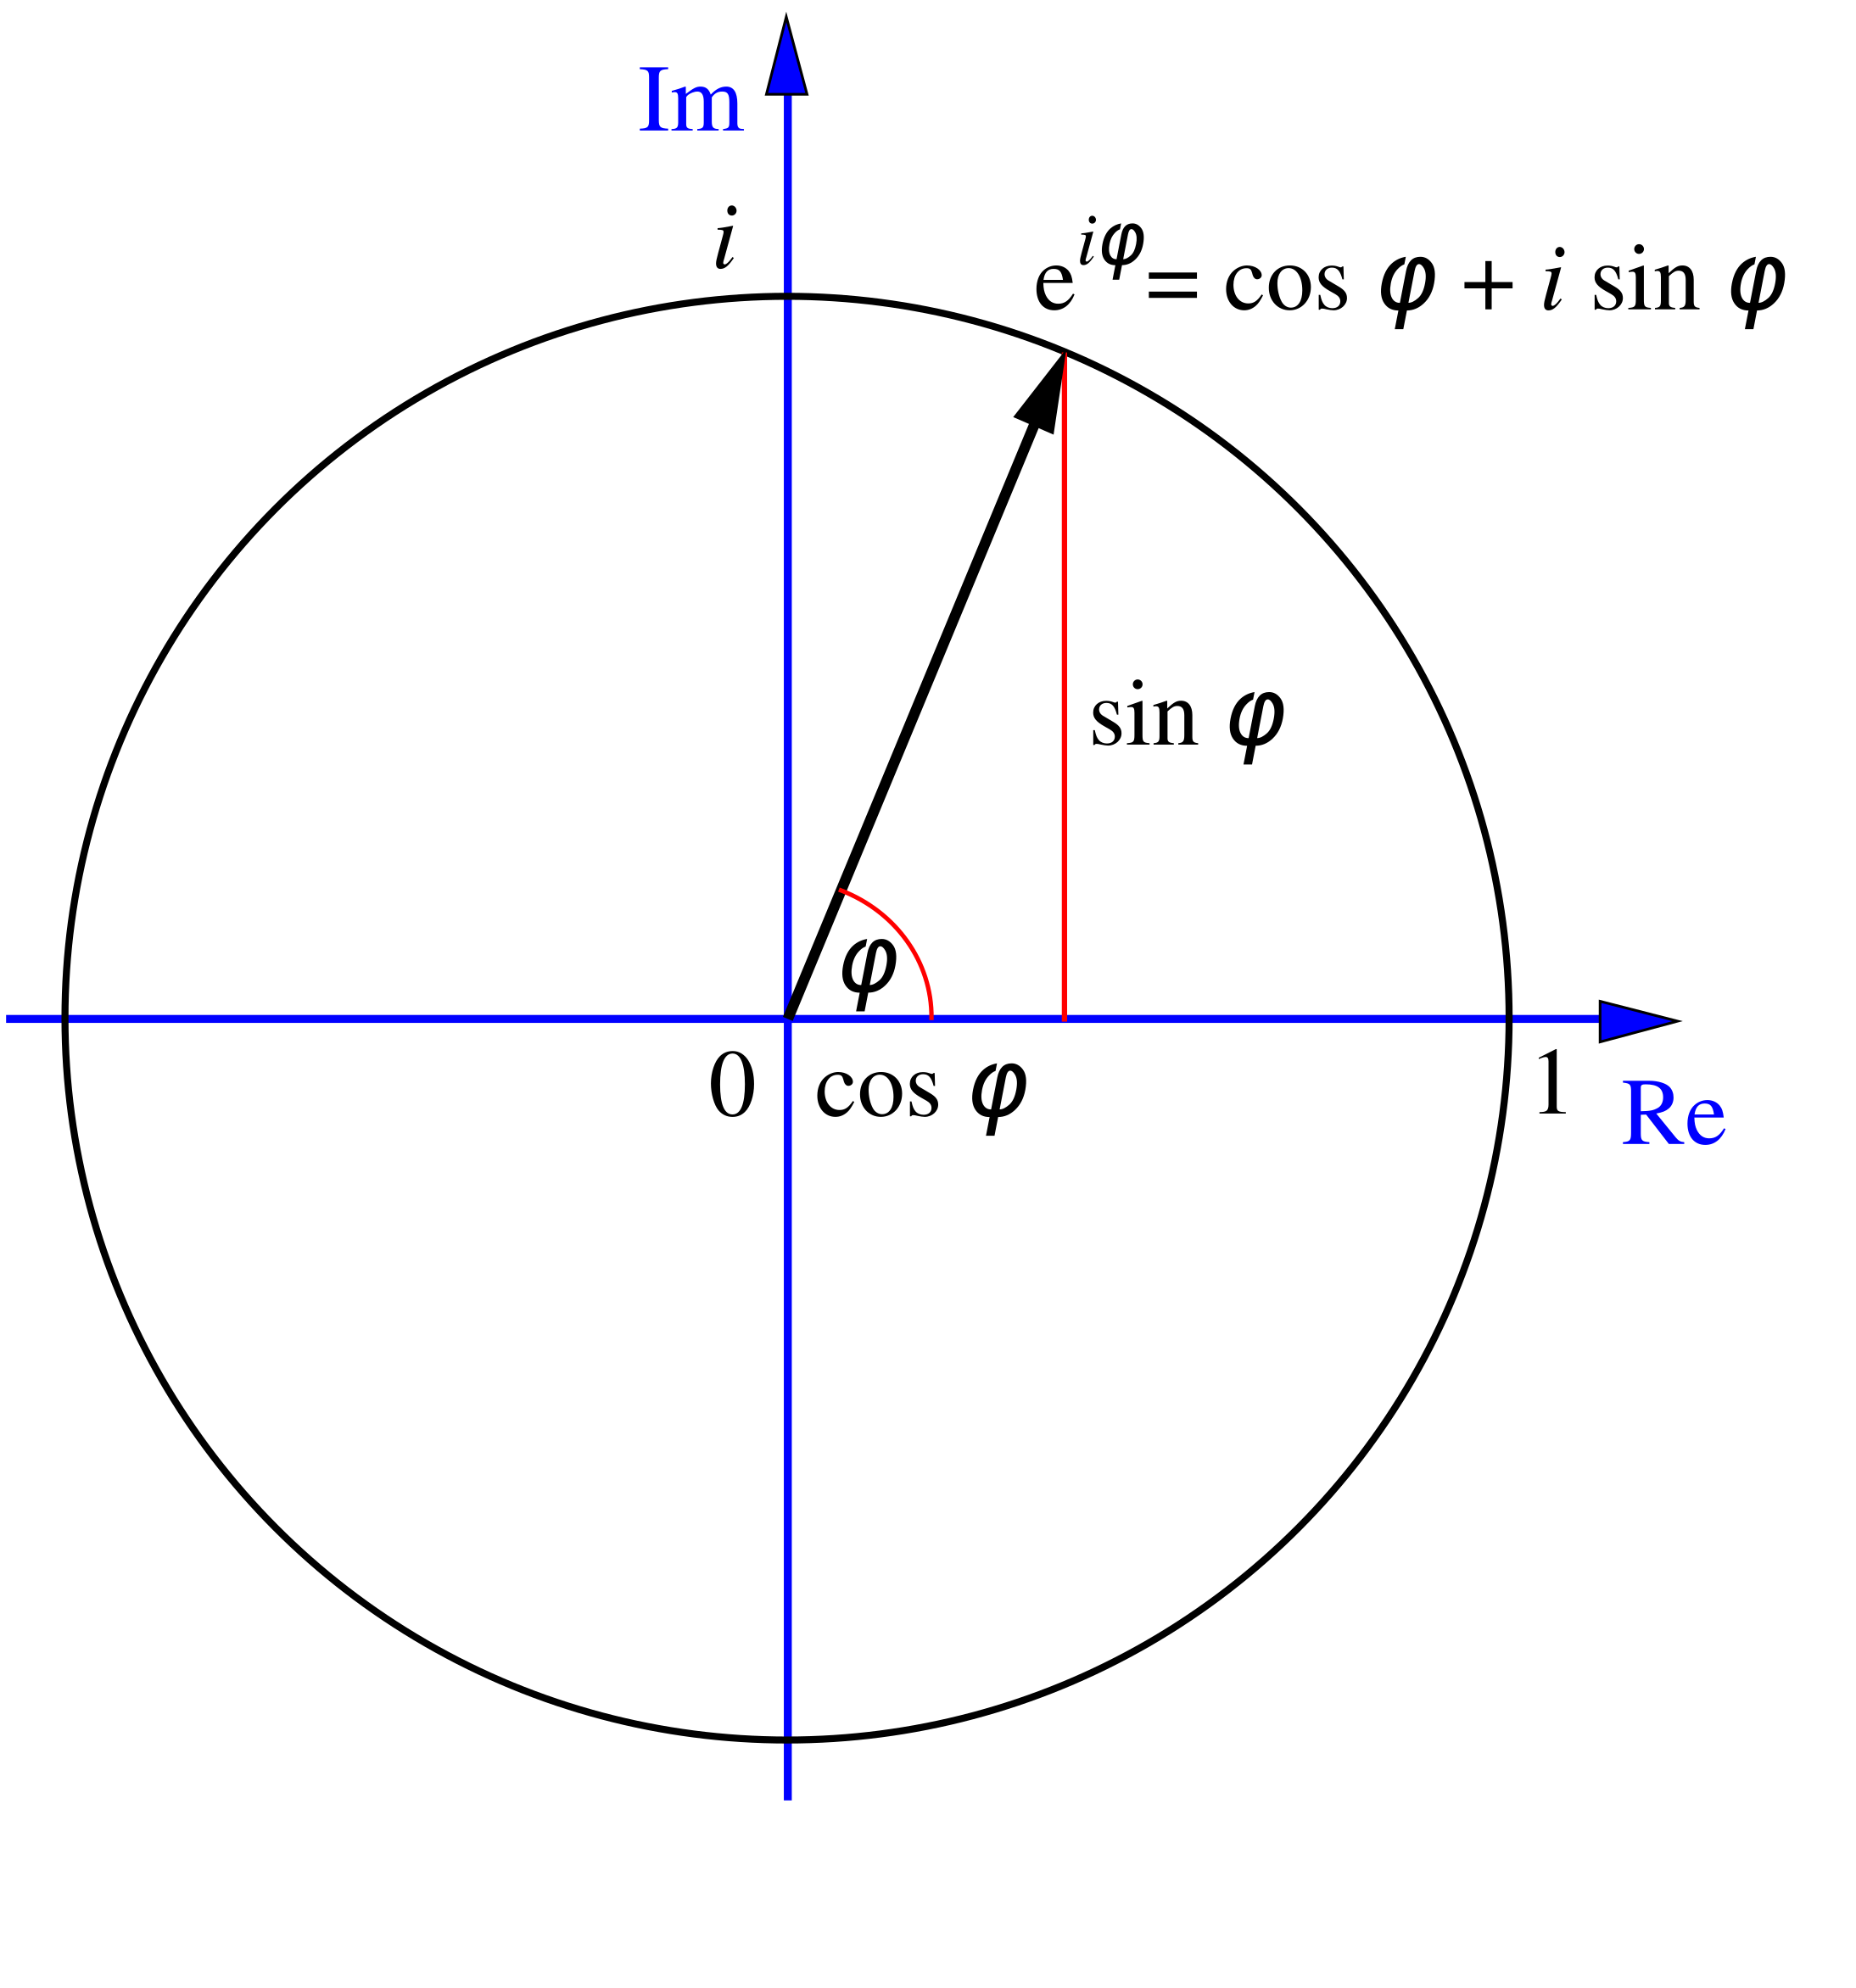
\includegraphics[width=0.4\textwidth]{images/euler_s_formula.png}
	\caption{Euler's formula Interpretation}
\end{wrapfigure}
This formula can be interpreted as saying that the function \(e^{j \varphi}\) is
a unit complex number, i.e., it traces out the unit circle in the complex plane
as \(\varphi\) ranges through the real numbers. Here \(\varphi\) is the angle
that a line connecting the origin with a point on the unit circle makes with the
positive real axis, measured counterclockwise and in radians.
\bigbreak
The original proof is based on the Taylor series expansions of the exponential
function \(e^z\) (where \(z\) is a complex number) and of \(sin(x)\) and
\(\cos(x)\) for real numbers \(x\). In fact, the same proof shows that Euler's
formula is even valid for all complex numbers \(z\). 

%-------------------------------------------------------------------------------
% Subsection 5: Euler's formula and Complex Numbers
%-------------------------------------------------------------------------------

\subsection{Euler's formula and Complex Numbers}
Using Euler's formula we can now write:
\[
	\boldsymbol{z = a + jb = c \cdot \cos(\varphi) + c \cdot sin(\varphi)
	\cdot j = c \cdot (\cos(\varphi) + j \cdot sin(\varphi)) =
	e^{j \varphi}}.
\]

%-------------------------------------------------------------------------------
% Subsubsection: Elementary Operations
%-------------------------------------------------------------------------------

\subsection{Elementary operations}
\subsubsection{Conjugate}
\begin{wrapfigure}{L}{0.4\textwidth}
	\centering
	\captionsetup{justification=centering}
	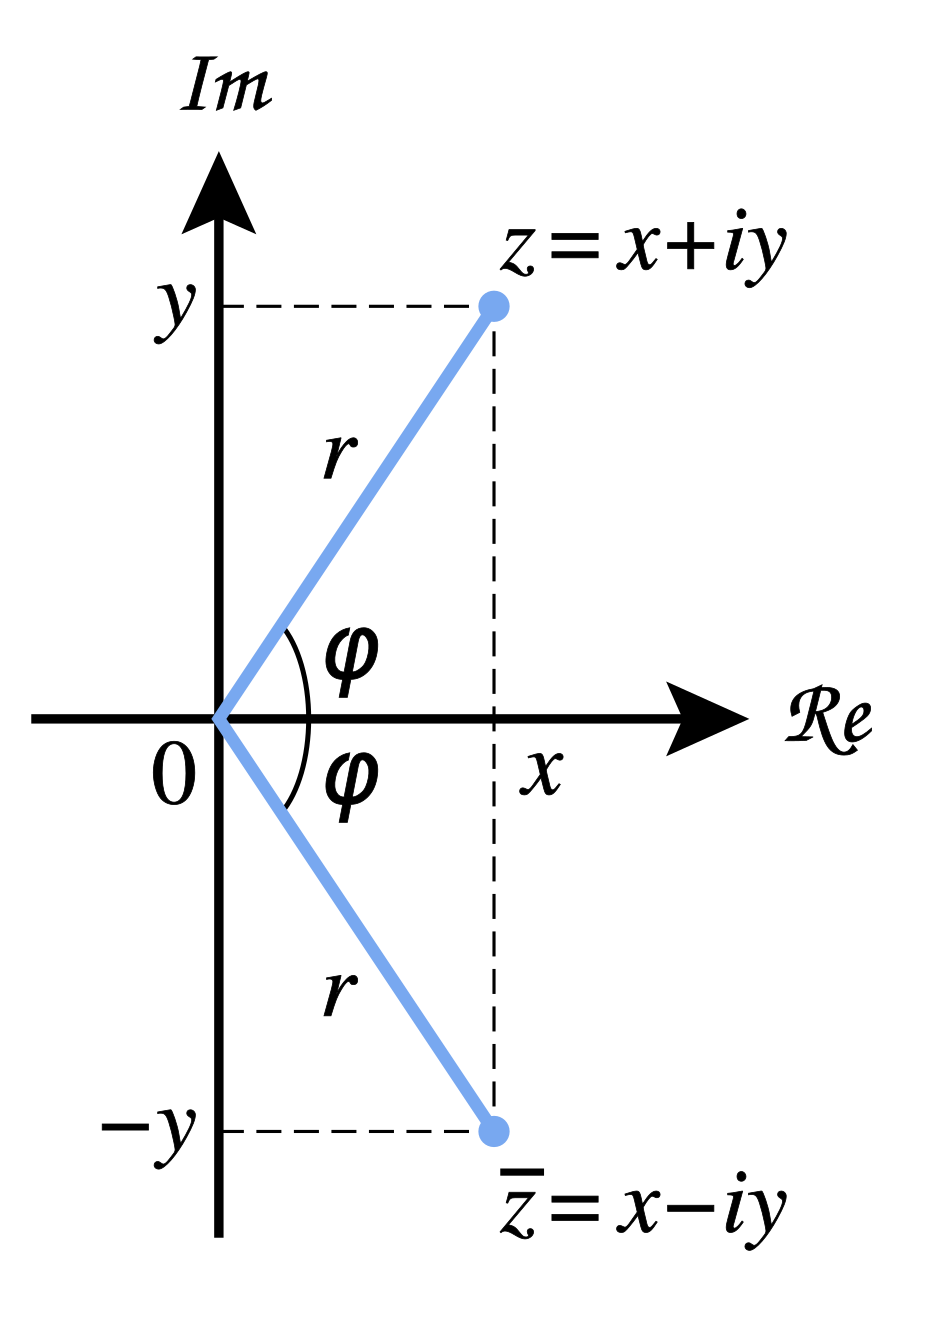
\includegraphics[width=0.4\textwidth]{images/complex_conjugate_picture.png}
	\caption{Geometric representation of z and its conjugate \(\conjugate{z}\)}
\end{wrapfigure}
The complex conjugate of the complex number \(z = a + jb\) is given by
\(a − jb\). It is denoted by either \(\conjugate{z}\) or \(z^*\). This unary
operation on complex numbers cannot be expressed by applying only their basic
operations addition, subtraction, multiplication and division.
\bigbreak
Geometrically, \(\conjugate{z}\) is the "reflection" of z about the real axis.
Conjugating twice gives the original complex number
\[
	\conjugate{\conjugate{z}},
\]
which makes this operation an involution. The reflection leaves both the real
part and the magnitude of \(z\) unchanged, that is
\[
	\Re(\conjugate{z}) = \Re(z) \quad and \quad \abs{\conjugate{z}} =
	\abs{z}.
\]
The imaginary part and the argument of a complex number \(z\) change their sign
under conjugation 
\[
	\Im(\conjugate{z}) = -\Im(z) \quad and \quad arg(\conjugate{z}) =
	-arg(z).
\]
\vspace{1.0cm}
\bigbreak
The real and imaginary parts of a complex number \(z = a + jb\) can be extracted
using the conjugation:
\[
	\boldsymbol{\Re(z) = a = \frac{z + \conjugate{z}}{2}} =
	\frac{a + jb + a - jb}{2} = \frac{2a}{2} = a.
\]
\[
	\boldsymbol{\Im(z) = b = \frac{z - \conjugate(z)}{2j}} =
	\frac{a + jb - a + jb}{2j} = \frac{2jb}{2j} = b.
\]
Moreover, a complex number is real if and only if it equals its own conjugate. 
\[
	z = \conjugate{z} \quad \rightarrow \quad z \in \mathbb{R}
\]

%-------------------------------------------------------------------------------
% Subsubsection: Additions and subtraction
%-------------------------------------------------------------------------------

\subsubsection{Addition and subtraction}
Two complex numbers \(z_1\) and \(z_2\) are most easily added by separately
adding their real and imaginary parts of the summands. That is to say:
\[
	z_1 + z_2 = a_1 = jb_1 + a_2 + jb_2 = (a_1 + a_2) + j(b_1 + b_2).
\]
Similarly, subtraction can be performed as
\[
	z_1 - z_2 = a_1 + jb_1 - (a_2 + jb_2) = (a_1 - a_2) +j(b_1 - b_2).
\]
\textbf{Please keep in mind that this is completely wrong:}
\[
	z_1 = c_1 \cdot e^{j \varphi_1} \quad , \quad z_2 = c_2
	\cdot e^{j \varphi_2}
\]
\[
	z_1 + z_2 = c_1 \cdot e^{j \varphi_1} + c_2 \cdot e^{j \varphi_2} =
	(c_1 + c_2) \cdot e^{j(\varphi_1 + \varphi_2)}
\]
\textbf{As a matter of fact:}
\[
	c_1 \cdot e^{j \varphi_1} = c_1 \cdot \cos(\varphi_1) + j \cdot
	c_1 \cdot sin(\varphi_1),
\]
\[
	c_2 \cdot e^{j \varphi_2} = c_2 \cdot \cos(\varphi_2) + j \cdot
	c_2 \cdot sin(\varphi_2),
\]
\[
	c_1 \cdot e^{j \varphi_1} + c_2 \cdot e^{j \varphi_2} = c_1 \cdot
	\cos(\varphi_1) + c_2 \cdot \cos(\varphi_2) + j \cdot
	(c_1 \cdot sin(\varphi_1) + c_2 \cdot sin(\varphi_2)),
\]
\textbf{while:}
\[
	(c_1 + c_2) \cdot e^{j (\varphi_1 + \varphi_2)} = (c_1 + c_2) \cdot
	(\cos(\varphi_1 + \varphi_2) + j \cdot sin(\varphi_1 + \varphi_2)) =
\]
\[
	c_1 \cdot \cos(\varphi_1 + \varphi_2) + c_2 \cdot
	\cos(\varphi_1 + \varphi_2) + j \cdot (c_1 \cdot
	sin(\varphi_1 + \varphi_2) + c_2 \cdot sin(\varphi_1 + \varphi_2)),
\]
\textbf{and:}
\[
	\cos(\varphi_1 + \varphi_2) \neq \cos(\varphi_1) + \cos(\varphi_2).
\]

%-------------------------------------------------------------------------------
% Subsubsection: Multiplication
%-------------------------------------------------------------------------------

\subsubsection{Multiplication}
Since the real part, the imaginary part, and the indeterminate \(i\) in a
complex number are all considered as numbers in themselves, two complex numbers,
given as \(z_1 = a_1 + j b_1\) and \(z_2 = a_2 + j b_2\) are multiplied under
the rules of the distributive property, the commutative properties and the
defining property \(i^{2} = -1\) in the following way
\[
	z_1 \cdot z_2 = (a_1 + j b_1) \cdot (a_2 + j b_2) =
\]
\[
	a_1 a_2 + j a_1 b_2 + j b_1 a_2 + (jj) b_1 b_2 = (a_1 a_2 + b_1 b_2) +
	j \cdot (a_1 b_2 + b_1 a_2).
\]
\textbf{The cartesian form is convenient for additions and subtractions but not
for multiplications.}

%-------------------------------------------------------------------------------
% Subsubsection: Multiplying a complex number by j
%-------------------------------------------------------------------------------

\subsubsection{Multiplying a complex number by j}
In our goal toward finding a geometric interpretation of complex multiplication,
let's consider next multiplying an arbitrary complex number \(z = a + jb\) by
\(j\):
\[
	z \cdot j = (a + jb) \cdot j = -b + ja
\]
\bigbreak
\begin{wrapfigure}{L}{0.4\textwidth}
	\centering
	\captionsetup{justification=centering}
	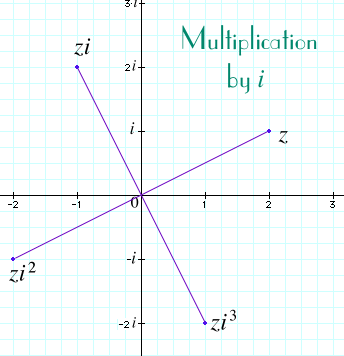
\includegraphics[width=0.4\textwidth]{images/multiply_by_i.png}
	\caption{Multiplying by i}
\end{wrapfigure}
Let's interpret this statement geometrically. The point \(z\) in \(\mathbb{C}\)
is located $a$ units to the right of the imaginary axis and $b$ units above the
real axis. The point $z \cdot j$ is located $b$ units to the left, and $a$ units
above. What has happened is that multiplying by $j$ has rotated the point $z$
$90^{\degree}$ counterclockwise around the origin to the point $zj$. Stated more
briefly, multiplication by $j$ gives a $90^{\degree}$ counterclockwise rotation
about 0. You can analyze what multiplication by $-j$ does in the same way.
You'll find that multiplication by $-j$ gives a $90^{\degree}$ clockwise
rotation about 0. When we don't specify counterclockwise or clockwise when
referring to rotations or angles, we'll follow the standard convention that
counterclockwise is intended. Then we can say that multiplication by $-j$ gives
a $-90^{\degree}$ rotation about 0, or if you prefer, a $270^{\degree}$ rotation
about 0.

%-------------------------------------------------------------------------------
% Section 2: The Field C of Complex Numbers
%-------------------------------------------------------------------------------

\newpage
\section{The Field C of Complex Numbers}
Before continuing with signal processing, I want to spend some time talking
about the field of complex numbers $\mathbb{C}$. The motivation for this is to
try and provide a much more formal definition of the field $\mathbb{C}$ than the
one roughly introduced in the previous section which represents the minimal
concepts required for the contents of the following pages. You can simply skip
over this section if you are not interested or have previous knowledge.

%-------------------------------------------------------------------------------
% Subsection: Naive introduction to the field C
%-------------------------------------------------------------------------------

\subsection{Naive introduction to the field C}
The usual way to quickly start with complex numbers is to say that we introduce
a new object, which I will call $j$ (mathematicians use $i$), such that the
following \textit{characteristic} property holds:
\[
	i^2 = -1.
\]
Now, having this object at my disposal, I can easily define the set of complex
numbers as the set with elements of the form $x + iy$ where $x$, $y$ are our
familiar real numbers:
\[
	\mathbb{C} \coloneqq \{x + iy : x,y \in \mathbb{R}, i^2 = -1\}.
\]
After this, using the usual rules of arithmetic operations as applied to the
real numbers, I can define the four fundamental operations for the complex
numbers as well. And I therefore have arithmetic in the set of complex numbers.
\bigbreak\noindent
The definition we just saw and the one used in the previous section are,
however, not really satisfactory, because they \textit{do not explain} what
$i$ is, and hence we get a sense of mystery here (and hence the name "imaginary"
numbers). But there is actually nothing imaginary about complex numbers, as was
realized by Gauss and others, if we identify them with the elements of our
familiar $\mathbb{R}^2$ and add a little more. This is the first formal
introduction for the set of complex numbers $\mathbb{C}$ I will provide in the
subsection \textbf{Definition of the field C} (as a side remark I note that
there are other ways to define complex numbers, but this one is arguably the
most natural). A second rigorous definition using matrices is provided in the
section \textbf{Constructing the complex numbers via the arithmetic of 2x2
matrices}.

%-------------------------------------------------------------------------------
% Subsection: Definition of the field C
%-------------------------------------------------------------------------------

\subsection{Definition of the field C}
\textit{The set of complex numbers, which is denoted by $\mathbb{C}$, is, by
definition, $\mathbb{R}^2$, this is, the set of all vectors with two real
coordinates, on which the operation of addition and multiplication are defined
as follows}
\[
	(x_1, y_1) + (x_2, y_2) = (x_1 + x_2, y_1 + y_2),
\]
\[
	(x_1, y_1) \cdot (x_2, y_2) = (x_1 x_2 - y_1 y_2, x_1 y_2 + y_1 x_2).
\]
Definitely, the multiplication rule should look a little strange at the
beginning, but of course the motivation comes from the previous subsection.
\bigbreak\noindent
\textit{The set $\mathbb{C}$, defined with such an addition and multiplication,
is a field. That is, it can be proved that for any
$z_1, z_2, z_3 \in \mathbb{C}$, we have}
\[
	z_1 + z_2 = z_2 + z_1,
\]
\[
	(z_1 + z_2) + z_3 = z_1 + (z_2 + z_3),
\]
\[
	z_1 z_2 = z_2 z_1,
\]
\[
	(z_1 z_2) z_3 = z_1 (z_2 z_3),
\]
\textit{there is a unique element $0 \in \mathbb{C}$ such that}
\[
	z_1 + 0 = z_1,
\]
\textit{for any $z_1 \in \mathbb{C}$ there is $-z_1 \in \mathbb{C}$ such that}
\[
	z_1 + (-z_1) = 0,
\]
for any nonzero $z \in \mathbb{C}$ there is $z^{-1} \in \mathbb{C}$ such that
\[
	z z^{-1} = 1.
\]
It should be clear that above $0 = (0, 0)$, where the $0$ on the left of the
equal sign is the complex zero, whereas the ones used in the round brackets are
in $\mathbb{R}$.
\bigbreak
Now, consider the following equation
\[
	z^2 + 1 = 0.
\]
Here $1$ and $0$ and the complex unit and the complex zero. We all know  that
this equation has  no real roots. But I claim that it has two complex roots
being $(0, 1)$ and $-(0, 1)$. This can easily be checked by substitution
according to the definition we provided for our addition and multiplication
(just keep in mind that .

%-------------------------------------------------------------------------------
% Subsection: Constructing the complex numbers via the arithmetic of 2x2 
% matrices
%-------------------------------------------------------------------------------

\subsection{Constructing the complex numbers via the arithmetic of 2x2 matrices}
\improvement[inline]{To be continued.}

%-------------------------------------------------------------------------------
% Chapter 2: Concetti Preliminari
%-------------------------------------------------------------------------------

\chapter{Concetti Preliminari}
\epigraph{
	"Anyone who has never made a mistake has never tried anything new."
}{--- \textup{Albert Einstein}}

Di seguito alcune definizioni essenziali necessarie per poter comprendere i
contenuti presentati nei capitoli successivi.

%-------------------------------------------------------------------------------
% Section: Introduzione allo studio dei segnali
%-------------------------------------------------------------------------------

\section{Introduzione allo studio dei segnali}
La teoria dei segnali studia le propriet\`a matematiche e statistiche dei
segnali, definiti come funzioni matematiche del tempo. In generale, un segnale
\`e una variazione temporale dello stato fisico di un sistema o di una grandezza
fisica (potenziale o corrente elettrica per segnali elettrici, parametri di
campo elettromagnetico per segnali radio) che serve per rappresentare e
trasmettere messaggi ovvero informazione a distanza; il sistema in questione
pu\`o essere il pi\`u disparato. In elettronica un segnale viene dunque studiato
attraverso un modello matematico o funzione in cui il tempo (o il suo inverso,
la frequenza) \`e considerato variabile indipendente.
\bigbreak
Un segnale \`e \textit{una qualunque grandezza fisica variabile cui \`e
associata una informazione}.
\bigbreak
In generale esistono diversi tipi di segnali, ma tutti sono accomunati
dall'essere in natura segnali casuali e continui e quasi mai deterministici. La
teoria dei segnali studia la rappresentazione dei segnali in modo da poter poi
manipolarli e trattarli matematicamente. Questa rappresentazione richiede l'uso
di matematica astratta e, nel caso di segnali stocastici, della teoria della
probabilit\`a.
\bigbreak
La teoria si suddivide in due grandi branche a seconda del tipo di segnale in
esame: i "segnali determinati" o deterministici, di cui è possibile predire il
valore in un qualunque istante a piacere, e i "segnali stocastici" o aleatori,
il cui valore non \`e prevedibile, ma su cui \`e possibile ottenere soltanto
delle propriet\`a statistiche e che rientrano nella pi\`u vasta tematica dei
processi aleatori o stocastici.
\bigbreak
Nella trasmissione di informazione a distanza (telecomunicazione) i segnali
determinati vengono utilizzati per la modulazione tramite portante, mentre i
segnali contenenti l'informazione sono invece segnali aleatori, quindi processi
stocastici, dal momento che l'informazione viaggia sotto forma di "innovazione"
ovvero varia in maniera aleatoria nel tempo.
\bigbreak
I segnali periodici possono essere trattati mediante l'astrazione in uno spazio
vettoriale lineare quale lo spazio di Hilbert e quindi con l'utilizzo della
serie di Fourier. Per quanto riguarda i segnali non periodici, questi
necessitano della trasformata di Fourier.
\bigbreak
Altra suddivisione \`e quella in "segnali continui" e "segnali discreti". Ad
essi si associano rispettivamente le comunicazioni analogiche e le comunicazioni
digitali.
\bigbreak
Parte della teoria dei segnali \`e intimamente connessa con la teoria dei
sistemi giacch\'e molti segnali transitano come input in sistemi che elaborano
ovvero trasformano il segnale in ingresso restituendo in uscita un certo output.
Centrale \`e anche l'analisi di Fourier ovvero l'analisi spettrale. 

%-------------------------------------------------------------------------------
% Subsection: Prorieta' elementari dei segnali determinati
%-------------------------------------------------------------------------------

\subsection{Propriet\`a elementari dei segnali determinati}
Limitiamo per il momento la nostra attenzione ai segnali determinati e definiamo
alcune grandezze di fondamentale importanza per il prosieguo dello studio.
Supponiamo di disporre di un resistore di resistenza $R$ attraversato da una
corrente $i(t)$; l'espressione della potenza istantanea dissipata sul resistore
per effetto Joule \`e, come \`e noto, $Ri^2(t)$. Osserviamo quindi la
proporzionalit\`a tra la potenza istantanea e il \textit{quadrato} del segnale;
il coefficiente di proporzionalit\`a \`e legato al particolare esempio.
Estendendo in maniera astratta tale definizione, diremo che al segnale $x(t)$
\`e associata una potenza istantanea \textit{normalizzata} (aggettivo che
verr\`a poi sistematicamente omesso) pari a
\begin{equation}
	P_x(t) = P_x \triangleq \abs{x(t)}^2.
\end{equation}
Inoltre, tornando all'esempio del resistore, l'energia totale dissipata per
effetto del passaggio della corrente $i(t)$ \`e pari a
$\int\displaylimits_{-\infty}^{+\infty} Ri^2(t) \dt$. Conseguentemente,
definiremo l'\textit{energia} associata al segnale $x(t)$ come
\begin{equation}
	E_x(t) = E_x \triangleq \int\displaylimits_{-\infty}^{+\infty}
	\abs{x(t)}^2 \dt = \int\displaylimits_{-\infty}^{+\infty} P_x(t) \dt
\end{equation}
purch\`e l'integrale risulti convergente (cio\`e $E_x < \infty$). La definizione
di energia, bench\`e meno intuitiva, viene banalmente estesa anche ai segnali a
tempo discreto:
\begin{equation}
	E_x \triangleq \sum_{n = -\infty}^{+\infty} \abs{x[n]}^2 < \infty.
\end{equation}
Per tutti i segnali \textit{fisici} (cio\`e effettivamente osservati)
l'integrale (o la sommatoria) che definisce l'energia risulta convergente,
poich\`e ogni segnale proveniente da un sistema fisico \`e portatore di
\textit{energia finita}. Molto spesso per\`o conviene considerare
\textit{modelli ideali} di segnale, ovvero segnali idealizzati non esistenti in
natura, ma assai utili per approssimare casi reali.\\
\\
Consideriamo ora un generico segnale $x(t)$ a valori limitati ma energia
infinita, e costruiamo il segnale $x_T(t)$ con una operazione di
\textit{troncamento} come segue:
\begin{equation}
	x_T(t) = \begin{cases}
			x(t) \quads{2} \abs{t} \leq T/2\\
			0 \quads{4} altrove
		 \end{cases}
\end{equation}
Se indichiamo con $E_{x_T}$ l'energia di $x_T(t)$, \`e chiaro che in generale
$E_{x_T} < \infty$ poich\`e il segnale \`e diverso da zero e assume valori
finiti solo su di un intervallo limitato. Altrettanto chiaro \`e che se
ingrandiamo l'intervallo di osservazione per comprendere l'andamento di tutto il
segnale $x(t)$ (imponiamo cio\`e $T \rightarrow \infty$) otteniamo
$E_{x_T} \rightarrow \infty$. Introduciamo allora il concetto di
\textit{potenza} di un segnale: la potenza media del segnale $x_T(t)$ valutata
sull'intervallo di osservazione $\left[-T/2, T/2\right]$ \`e per definizione
pari all'energia di $x_T(t)$ rapportata alla durata dell'intervallo stesso:
\begin{equation}
	P_{x_T} \triangleq \frac{E_{x_T}}{T}.
\end{equation}
Siamo ora in grado di estendere a $x(t)$ questa definizione di \textit{potenza
media} attraverso un'operazione di passaggio al limite:
\begin{equation}\label{eq:signal_power}
	P_x \triangleq \lim_{T \rightarrow \infty} P_{x_T} =
	\lim_{T \rightarrow \infty} \frac{E_{x_T}}{T} =
	\lim_{T \rightarrow \infty} \frac{1}{T} \int\displaylimits_{-T/2}^{T/2}
	\abs{x(t)}^2 \dt.
\end{equation}
Analogamente a quanto visto per l'energia di un segnale, per i segnali a tempo
discreto abbiamo
\begin{equation}
	P_x \triangleq \lim_{N \rightarrow \infty} \frac{1}{2N + 1}
	\sum_{n = -N}^{N} \abs{x[n]}^2
\end{equation}
dove la notazione \`e autoesplicativa.
Talvolta torna utile usare il \textit{valore efficace} di un segnale a potenza
finita, definito sia per i segnali a tempo continuo, sia per quelli a tempo
discreto come
\begin{equation}
	x_{eff} \triangleq \sqrt{P_x}.
\end{equation}
Ricordiamo che il valore efficace di un dato segnale (chiamato nei paesi
anglosassoni RMS, \textit{Root Mean Square}) si pu\`o interpretare come quel
valore che dovrebbe assumere un segnale costante per avere la stessa potenza del
segnale dato.\\
Definiamo infine il \textit{valore medio temporale} di un segnale, che richiede
un procedimento al limite simile a quello appena visto relativamente alla
potenza:
\begin{equation}
	x_m \triangleq \lim_{T \rightarrow \infty} \frac{1}{T}
	\int\displaylimits_{-T/2}^{T/2} x(t) dt,
\end{equation}
\begin{equation}
	x_m \triangleq \lim_{N \rightarrow \infty} \frac{1}{2N + 1}
	\sum_{n = -N}^{N} x[n].
\end{equation}
Nell'ingegneria elettrica, il valore medio rappresenta la "componente continuo"
(cio\`e costante) attorno alla quale si svolge l'evoluzione del segnale.

%-------------------------------------------------------------------------------
% Subsubsection: Esercizio Lezione 12 Marzo 2018
%-------------------------------------------------------------------------------

\subsubsection{Esercizio 12 Marzo 2018}
Calcolare $E_y$, $P_y$, $y_{eff}$ e $y_m$ per la funzione $y(t)$ definita  come
\begin{equation}
	y(t) = x(t) - x(-t),
\end{equation}
dove $x(t)$ \`e definita come
\[
	x(t) = A e^{-t} \cdot u(t)
	\footnote{Il segnale canonico "gradino unitario" \`e presente
	nell'Appendice A: Segnali Canonici.}.
\]
Infine quindi
\begin{equation}
	y(t) = A e^{-t} \cdot u(t) - A e^{t} \cdot u(-t).
\end{equation}
\begin{figure}[H]
\centering
\captionsetup{justification=centering}
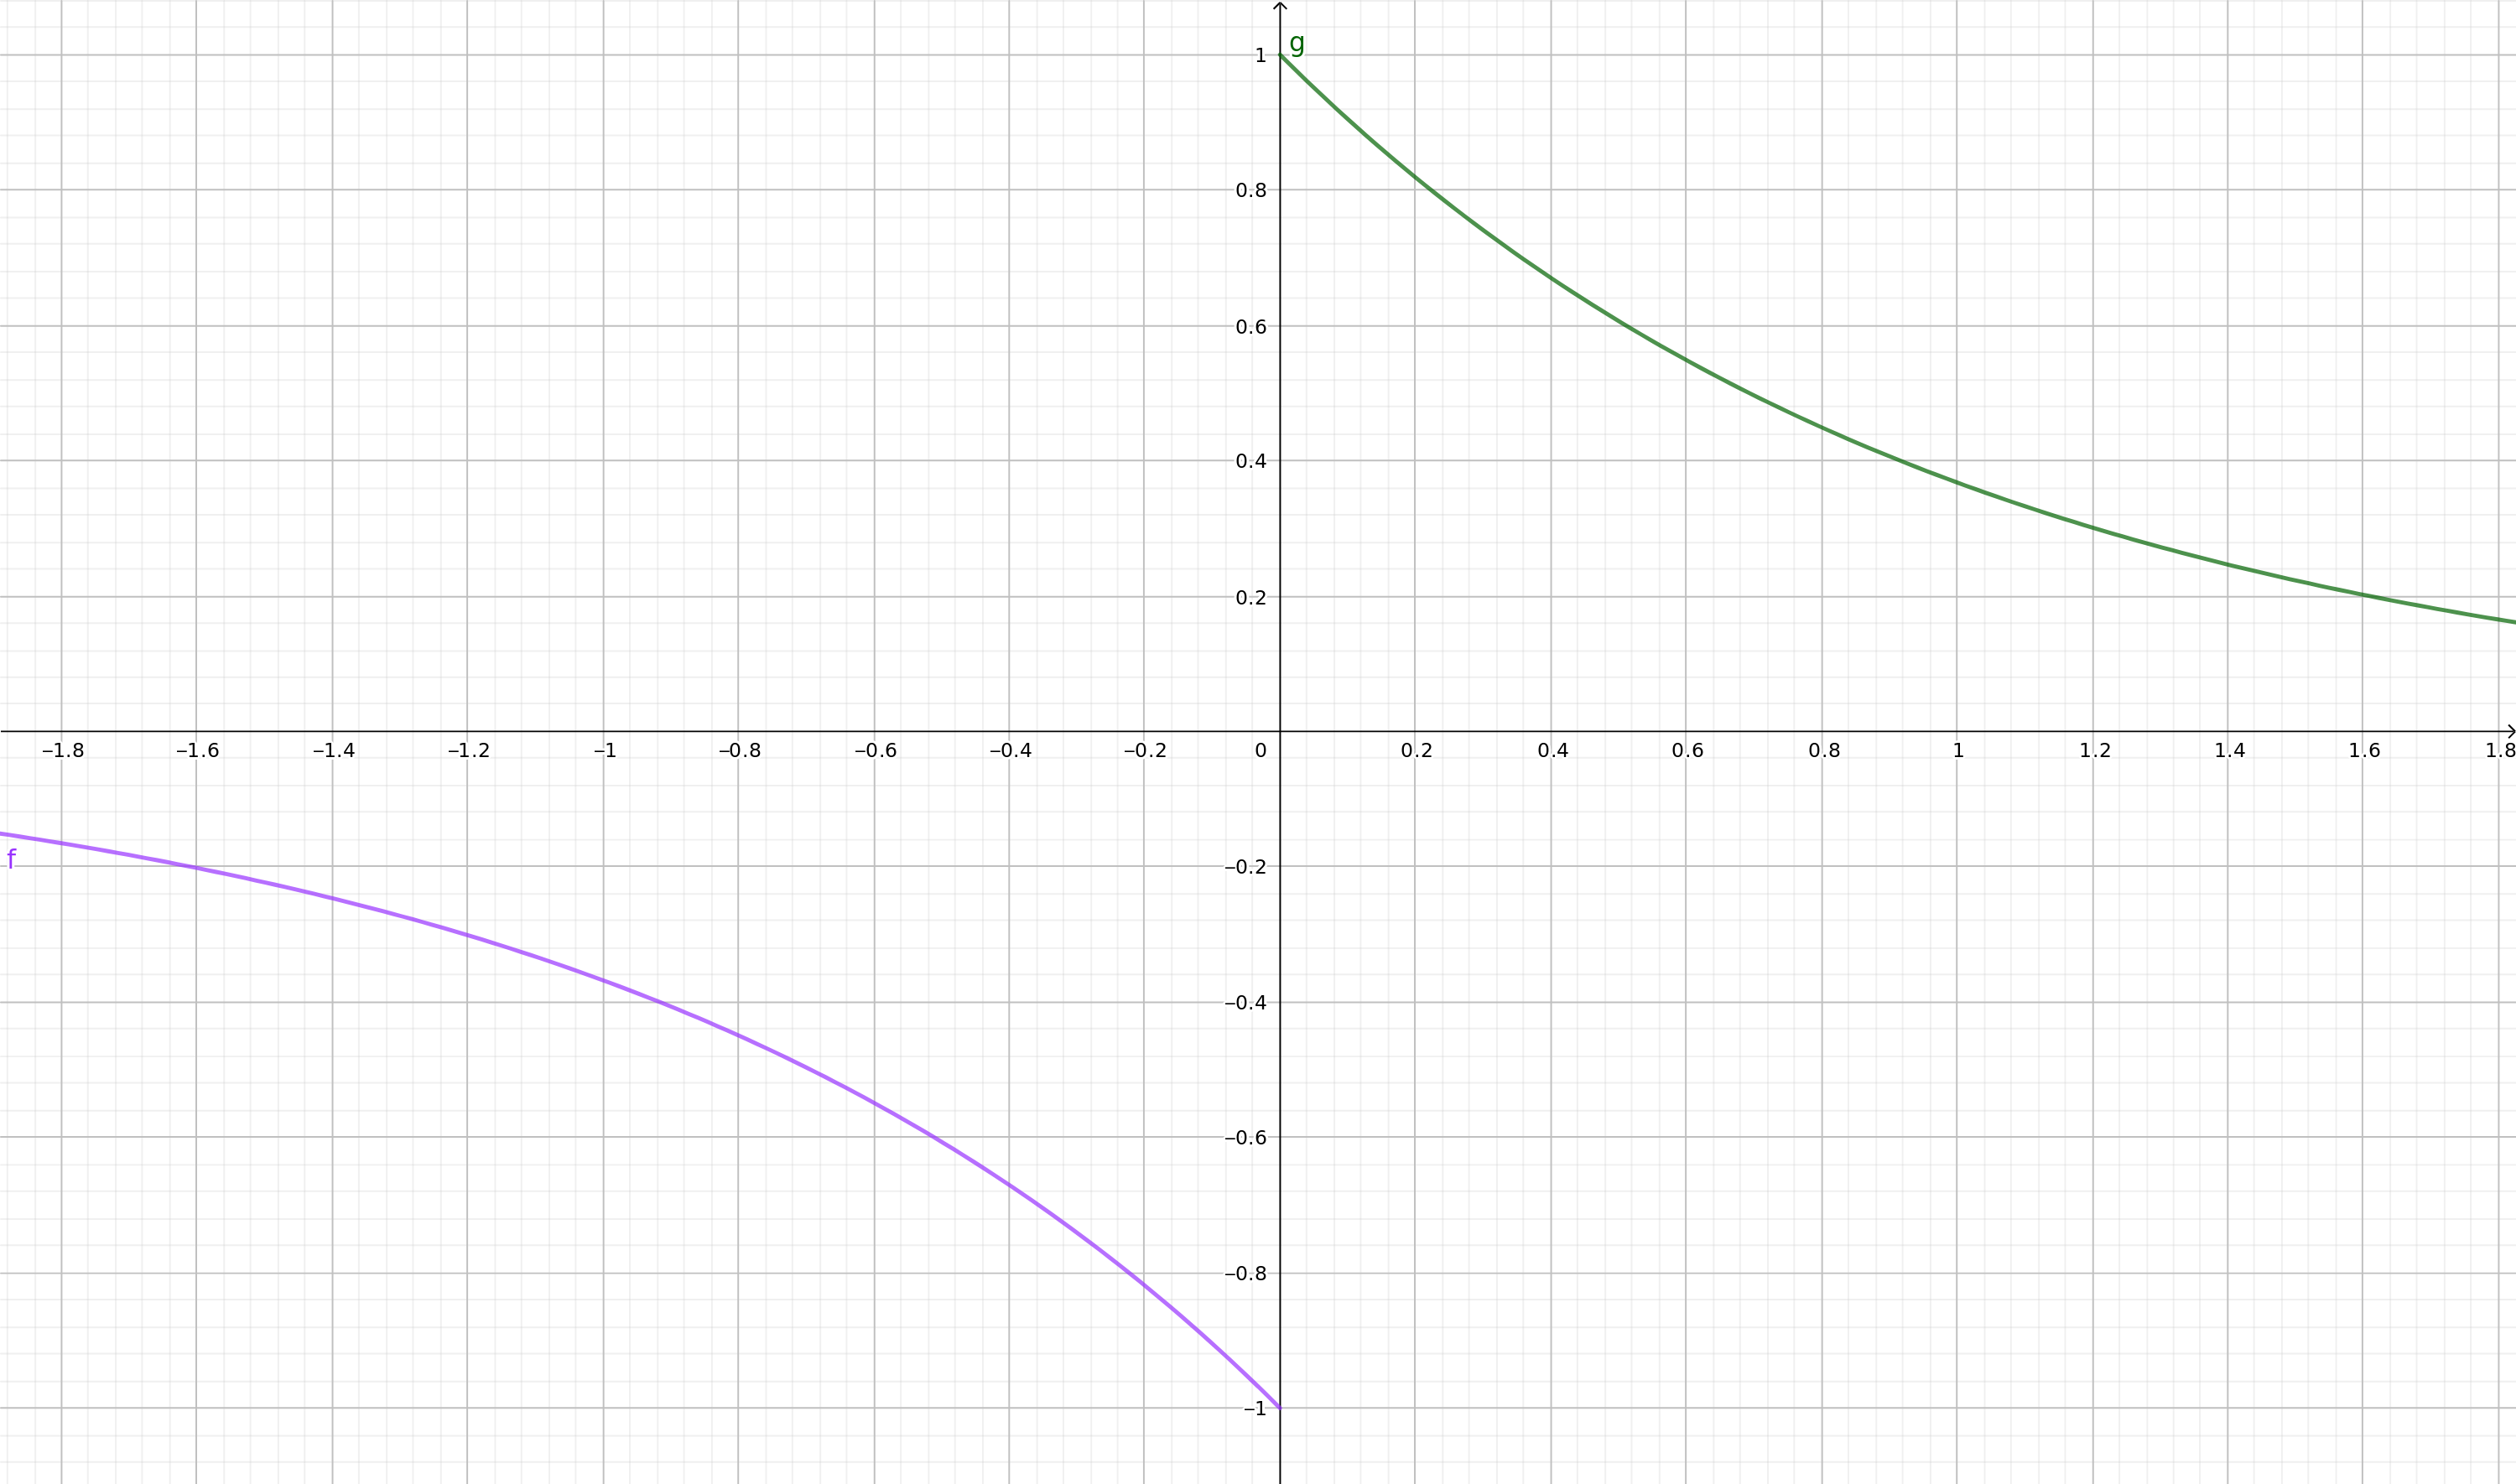
\includegraphics[width=1.0\textwidth]{images/esercizio_12_marzo_2018.png}
\caption{Grafico di $y(t)$ con $A = 1$.}
\end{figure}
Come possiamo vedere graficamente, il segnale gradino $u(t)$ fa si che la
funzione complessiva $y(t)$ si ottenga come contributo delle due funzioni
\[
	A e^{-t} \quads{2} t \rightarrow +\infty,
\]
e
\[
	-A e^{t} \quads{2} t \rightarrow -\infty.
\]
\textbf{Calcolo di $\boldsymbol{E_y}$}\\
\[
	E_y = \int\displaylimits_{-\infty}^{+\infty} \abs{y(t)}^2 \dt =
	\int\displaylimits_{-\infty}^{+\infty} \abs{x(t) - x(-t)}^2 \dt =
\]
\[
	= \int\displaylimits_{-\infty}^{+\infty} \abs{A e^{-t} \cdot u(t) -
	A e^{t} \cdot u(-t)}^2 \dt =
\]
\[
	= \int\displaylimits_{-\infty}^{0} \abs{A e^{-t} \cdot u(t) - A e^{t}
	\cdot u(-t)}^2 \dt + \int\displaylimits_{0}^{+\infty} \abs{A e^{-t}
	\cdot u(t) - A e^{t} \cdot u(-t)}^2 \dt =
\]
\[
	\footnote{Notiamo che $u(t) = 0$ $[-\infty, 0]$ e $u(-t) = 0$
	$[0, +\infty]$.}= \int\displaylimits_{-\infty}^{0} \abs{- A e^{t} \cdot
	u(-t)}^2 \dt + \int\displaylimits_{0}^{+\infty} \abs{A e^{-t} \cdot
	u(t)}^2 \dt =
\]
\[
	\footnote{Notiamo che $\abs{u(t)}^2 = \abs{u(-t)}^2 = 1$.}=
	\int\displaylimits_{-\infty}^{0} \abs{- A e^{t}}^2 \dt + 
	\int\displaylimits_{0}^{+\infty} \abs{A e^{-t}}^2 \dt = 
	\int\displaylimits_{-\infty}^{0} A^2 e^{2t} \dt + 
	\int\displaylimits_{0}^{+\infty} A^2 e^{-2t} \dt =
\]
\[
	= \int\displaylimits_{-\infty}^{0} A^2 e^{2t} \dt +
	\int\displaylimits_{0}^{+\infty} A^2 e^{-2t} \dt =
	\int\displaylimits_{-\infty}^{+\infty} A^2 e^{-2\abs{t}} \dt =
\]
\[
	= 2 \int\displaylimits_{0}^{+\infty} A^2 e^{-2t} \dt = 2 A^2
	\int\displaylimits_{0}^{+\infty} e^{-2t} \dt = 2 A^2 \cdot
	\left(-\frac{1}{2} \left[e^{-2t} \right]_0^\infty\right) =
\]
\[
	2 A^2 \cdot \left(-\frac{1}{2} e^{-2\cdot(\infty)} - \left(-\frac{1}{2}
	e^{-2\cdot(0)}\right) \right) = 2 A^2 \cdot \frac{1}{2} = A^2.
\]
\bigbreak\noindent
\textbf{Calcolo di $\boldsymbol{P_y}$, $\boldsymbol{y_{eff}}$ e
$\boldsymbol{y_y}$}\\
Dato che $E_y = A^2 = K < \infty$ allora
\[
	P_y = 0,
\]
\[
	y_{eff} = 0,
\]
\[
	y_m = 0.
\]
\begin{proof}
\begin{equation}
\begin{split}
	P_y = \lim_{T \rightarrow \infty} \frac{1}{T}
	\int\displaylimits_{-T/2}^{T/2} \abs{y(t)}^2 \dt = 
	\quads{13}
	\\
	= \lim_{T \rightarrow \infty} \frac{1}{T}
	\int\displaylimits_{-T/2}^{T/2} \abs{A e^{-t} u(t) - A e^t u(-t)}^2
	\dt =
	\quads{10}
	\\
	= \lim_{T \rightarrow \infty} \frac{1}{T} \left[
		\int\displaylimits_{-T/2}^{0} \abs{A e^{-t} u(t) -
		A e^t u(-t)}^2 \dt + \int\displaylimits_{0}^{T/2}
		\abs{A e^{-t} u(t) - A e^t u(-t)}^2 \dt
	\right] =
	\\
	= \lim_{T \rightarrow \infty} \frac{1}{T} \left[
		\int\displaylimits_{-T/2}^{0} \abs{- A e^t u(-t)}^2 \dt +
		\int\displaylimits_{0}^{T/2} \abs{A e^{-t} u(t)}^2 \dt
	\right] =
	\quads{7}
	\\
	= \lim_{T \rightarrow \infty} \frac{1}{T} \left[
		\int\displaylimits_{-T/2}^{0} A^2 e^{2t} \dt + 
		\int\displaylimits_{0}^{T/2} A^2 e^{-2t} \dt
	\right] =
	\lim_{T \rightarrow \infty} \frac{1}{T} \int\displaylimits_{-T/2}^{T/2}
	A^2 e^{-2\abs{t}} \dt =
	\quads{3}
	\\
	= \lim_{T \rightarrow \infty} \frac{1}{T} 2 \int\displaylimits_{0}^{T/2}
	A^2 e^{-2t} \dt = \lim_{T \rightarrow \infty} \frac{1}{T} 2 A^2
	\int\displaylimits_{0}^{T/2} e^{-2t} \dt =
	\quads{8}
	\\
	= \lim_{T \rightarrow \infty} \frac{1}{T} 2 A^2
	\int\displaylimits_{0}^{T/2} \frac{1}{2} \cdot 2 \cdot e^{-2t} \dt =
	\lim_{T \rightarrow \infty} \frac{1}{T} A^2 \int\displaylimits_{0}^{T/2}
	2 \cdot e^{-2t} \dt =
	\quads{7}
	\\
	= \lim_{T \rightarrow \infty} \frac{1}{T} A^2 \left[
		e^{-2t}\right]_0^{T/2} = \lim_{T \rightarrow \infty}
		\frac{A^2}{T} \left[e^{-T} - 1\right] = 0.
	\quads{8}
\end{split}
\end{equation}
\begin{equation}
	y_eff = \sqrt{P_y} = 0.
\end{equation}
\begin{equation}
\begin{split}
	y_m = \lim_{T \rightarrow \infty} \frac{1}{T}
	\int\displaylimits_{-T/2}^{T/2} y(t) \dt = \lim_{T \rightarrow \infty}
	\frac{1}{T} \int\displaylimits_{-T/2}^{T/2} x(t) - x(-t) \dt =
	\quads{4}
	\\
	= \lim_{T \rightarrow \infty} \frac{1}{T}
	\int\displaylimits_{-T/2}^{T/2} A e^{-t} u(t) - A e^{t} u(-t) \dt =
	\quads{7}
	\\
	= \lim_{T \rightarrow \infty} \frac{1}{T} \left[
		\int\displaylimits_{-T/2}^{0} A e^{-t} u(t) - A e^{t} u(-t) \dt
		+ \int\displaylimits_{0}^{T/2} A e^{-t} u(t) - A e^{t} u(-t) \dt
	\right] =
	\\
	= \lim_{T \rightarrow \infty} \frac{1}{T} \left[
		\int\displaylimits_{-T/2}^{0} - A e^{t} u(-t) \dt +
		\int\displaylimits_{0}^{T/2} A e^{-t} u(t) \dt
	\right] =
	\quads{4}
	\\
	= \lim_{T \rightarrow \infty} \frac{1}{T} \left[
		\int\displaylimits_{-T/2}^{0} - A e^{t} \dt +
		\int\displaylimits_{0}^{T/2} A e^{-t} \dt
	\right] =
	\quads{7}
	\\
	= \lim_{T \rightarrow \infty} \frac{1}{T} \left[
		-A \left(e^0 - e^{-T/2}\right) + A \left(-e^{-T/2} + e^0\right)
	\right] =
	\quads{5}
	\\
	= \lim_{T \rightarrow \infty} \frac{1}{T} \left[
		-A + Ae^{-T/2} - Ae^{-T/2} + A
	\right] = 0.
	\quads{6}
\end{split}
\end{equation}
\end{proof}

%-------------------------------------------------------------------------------
% Section: Segnali periodici a tempo continuo
%-------------------------------------------------------------------------------

\newpage
\section{Segnali periodici a tempo continuo}
Un segnale $x(t)$ \`e periodico se soddisfa la seguente relazione
\begin{equation}
	x(t) = x(t + T_0)
\end{equation}
per ogni valore della variabile $t$. La grandezza $T_0$ rappresenta il
\textit{periodo} del segnale che \`e legato alla \textit{frequenza di
ripetizione $f_0$} del segnale stesso dalla relazione
\begin{equation}
	f_0 = \frac{1}{T_0}.
\end{equation}
\textit{L'energia $E_x$} del segnale periodico \`e infinita:
\begin{equation}
\begin{split}
	E_x = \int\displaylimits_{-\infty}^{+\infty} \abs{x(t)}^2 \dt =
	\sum_{k = -\infty}^{+\infty}
	\int\displaylimits_{-T_0/2 + k T_0}^{T_0/2 + k T_0} \abs{x(t)}^2 \dt =
	\\
	= \sum_{k = -\infty}^{+\infty} E_{T_0} =
	\lim_{k \rightarrow \infty} k \cdot E_{T_0} = \infty.
	\quads{4}
\end{split}
\end{equation}
Dove si \`e posto
\begin{equation}
	E_{T_0} = \int\displaylimits_{-T_0/2 + k T_0}^{T_0/2 + k T_0}
	\abs{x(t)}^2 \dt.
\end{equation}
\textbf{Per la precedente (2.13) \`e di fondamentale importanza la seguente
considerazione:}
\begin{lemma}
L'integrale di una funzione periodica lungo intervalli pari al periodo stesso
della funzione \`e uguale indipendentemente dall'intervallo considerato.
\\
Ovvero, sia $x(t) = x(t + T_0)$ $\forall t$ un funzione periodica di periodo
$T_0$, allora
\begin{equation}
	\int\displaylimits_{0}^{T_0} x(t) \dt =
	\int\displaylimits_{b}^{b + T_0} x(t) \dt.
\end{equation}
\end{lemma}
\begin{proof}
Poniamo
\begin{equation}
	H(b) = \int\displaylimits_{b}^{b + T_0} x(t) \dt.
\end{equation}
Calcoliamo la derivata di $H(b)$:
\[
	\frac{dH(b)}{db} = x(b + T_0) - x(b) =
	\footnote{Essendo $x(t)$ periodica infatti risulta $x(b + T_0) = x(b)$.}
	\ 0.
\]
Ne segue che $H(b)$ \`e costante, in particolare $H(b) = H(0)$.
\end{proof}
In generale invece $x(t)$ ha \textit{potenza} $P_x$ finita, per calcolare la 
quale, non \`e necessario il procedimento di passaggio al limite definito dalla
\eqref{eq:signal_power}, ma \`e sufficiente calcolare
\begin{equation}
	P_x = \frac{1}{T_0} \int\displaylimits_{-T_0/2}^{T_0/2} \abs{x(t)}^2
	\dt.
\end{equation}
\begin{proof}
\begin{equation}
\begin{split}
	P_x = \lim_{T \rightarrow \infty} \frac{1}{T} 
	\int\displaylimits_{-T/2}^{T/2} \abs{x(t)}^2 \dt = 
	\lim_{k \rightarrow \infty} \frac{1}{kT_0} \cdot 
	\int\displaylimits_{-kT_0/2}^{kT_0/2} \abs{x(t)}^2 \dt =
	\\
	= \lim_{k \rightarrow \infty} \frac{1}{kT_0} \cdot k \cdot 
	\int\displaylimits_{-T_0/2}^{T_0/2} \abs{x(t)}^2 \dt = 
	\lim_{k \rightarrow \infty} \frac{1}{T_0} \cdot 
	\int\displaylimits_{-T_0/2}^{T_0/2} \abs{x(t)}^2 \dt =
	\\
	= \frac{1}{T_0} \int\displaylimits_{-T_0/2}^{T_0/2} \abs{x(t)}^2 \dt.
	\quads{8}
\end{split}
\end{equation}
\end{proof}
\textbf{Con segnali periodici \`e bene fare attenzione a non confondere il
periodo $T_0$ della funzione $x(t)$ con il troncamento $T$ della funzione
stessa.}
\bigbreak
Mentre il \textit{valore efficace} di un segnale periodico segue dalla
definizione della potenza $P_x$
\begin{equation}
	x_eff = \sqrt{P_x},
\end{equation}
analogamente a quanto visto per la potenza, l'espressione del \textit{valor
medio} si semplifica, per il segnale periodico $x(t)$, come segue:
\begin{equation}
	x_m = \frac{1}{T_0} \int\displaylimits_{-T_0/2}^{T_0/2} x(t) \dt.
\end{equation}
\begin{proof}
\begin{equation}
\begin{split}
	x_m = \lim_{T \rightarrow \infty} \frac{1}{T} 
	\int\displaylimits_{-T/2}^{T/2} x(t) \dt = \lim_{k \rightarrow \infty}
	\frac{1}{kT_0} \int\displaylimits_{-kT_0/2}^{kT_0/2} x(t) \dt =
	\\
	= \lim_{k \rightarrow \infty} \frac{1}{kT_0} k 
	\int\displaylimits_{-T_0/2}^{T_0/2} x(t) \dt = 
	\lim_{k \rightarrow \infty} \frac{1}{T_0} 
	\int\displaylimits_{-T_0/2}^{T_0/2} x(t) \dt =
	\quad
	\\
	= \frac{1}{T_0} \int\displaylimits_{-T_0/2}^{T_0/2} x(t) \dt.
	\quads{8}
\end{split}
\end{equation}
\end{proof}

%-------------------------------------------------------------------------------
% Subsection: Sviluppo in serie di Fourier in forma reale polare
%-------------------------------------------------------------------------------

\subsection{Sviluppo in serie di Fourier in forma reale polare}
Ci\`o premesso, ci poniamo una domanda: qual \`e il modo pi\`u appropriato di
procedere quando il segnale $x(t)$ \`e periodico con \textit{andamento
arbitrario}, e in particolare \textit{non sinusoidale}? La risposta a questo
quesito sta nella cosiddetta \textit{analisi di Fourier} che costituisce la
base della moderna teoria dei segnali. Infatti, sotto ipotesi piuttosto ampie,
che in seguito elencheremo, un segnale reale periodico qualunque pu\`o essere
espresso come \textit{somma di oscillazioni sinusoidali di ampiezza, frequenza e
fase opportune} cio\`e in una forma che richiami:
\begin{equation}\label{eq:periodic_signal_decomposition}
	x(t) = a_0 + a_1 \cos(2 \pi f_1 t + \vartheta_1) + a_2 \cos(2 \pi f_2 t
	+ \vartheta_2) + \dots
\end{equation}
In particolare, le frequenze di oscillazione includono in generale la "frequenza
zero" relative al termine costante, e sono \textit{multiple intere della
frequenza fondamentale $f_0$}, cosicch\'e la
\eqref{eq:periodic_signal_decomposition} diventa:\footnote{Il termine $A_0$ \`e
dato dal fatto che il coseno in $0$ valore $1$ mentre il seno vale $0$.}
\begin{equation}\label{eq:fourier_series_polar_form}
	x(t) = A_0 + 2 \sum_{n = 1}^{\infty} A_n \cos(2 \pi n f_0 t + \vartheta_n)
\end{equation}
dove per comodit\`a di notazione si \`e anche posto $A_0 = a_0$ e $2A_n = a_n$
per $n \geq 1$. Questa rappresentazione del segnale prende il nome di
\textit{sviluppo in seria di Fourier}; pi\`u precisamente la relazione
\eqref{eq:fourier_series_polar_form} costituisce l'\textit{espressione in forma
polare} dello sviluppo in serie di Fourier. Essa permette dunque di
rappresentare un segnale reale $x(t)$ come somma di una costante $A_0$ e di una
\textit{serie} il cui \textit{n}-esimo termine, detto \textit{n}-esima
\textit{oscillazione armonica} (o \textit{armonica tout-court}), ha ampiezza
$A_n > 0$, frequenza $nf_0$ (la \textit{n}-esima \textit{frequenza armonica}) e
fase iniziale $\vartheta_n$.
\bigbreak
Prima di procedere ulteriormente, da un punto di vista formale, \`e bene
dimostrare che la funzione $A_n \cos(2 \pi n f_0 t + \vartheta_n)$ sia
effettivamente periodica:
\[
	A_n \cos(2 \pi n f_0 t + \vartheta_n) = A_n \cos(2 \pi n f_0 (t - mT_0)
	+ \vartheta_n) \quad \forall m \in \mathbb{Z}.
\]
\begin{proof}
Ricordando che $f_0 \cdot T_0 = 1$ e che $T_{\cos(x)} = 2\pi$,
\begin{equation}
\begin{split}
	A_n \cos(2 \pi n f_0 (t - mT_0) + \vartheta_n) =
	\quads{5}
	\\
	= A_n \cos(2 \pi n f_0 t + \vartheta_n - 2 \pi n f_0 m T_0) =
	\quads{4}
	\\
	= A_n \cos(2 \pi n f_0 t + \vartheta_n - 2 \pi n m) = A_n
	\cos(2 \pi n f_0 t + \vartheta_n).
\end{split}
\end{equation}
\end{proof}
Evidentemente, ogni particolare segnale $x(t)$ sar\`a caratterizzato da
particolari insiemi di valori di $A_n$ e $\vartheta_n$. Dovremo quindi ricavare
formule utili per il calcolo delle ampiezze e delle fasi delle varie armoniche e
indicare condizioni matematiche che garantiscano la convergenza della serie
\eqref{eq:fourier_series_polar_form}. Il primo di questi problemi fu risolto dal
matematico L. Eulero attorno alla fine del 1700 in connessione con lo studio
delle corde vibranti. e fu ripreso alcuni anni pi\`u tardi da J.B. Fourier.
Quest'ultimo fu il primo a intuire l'importanza e la potenza della
rappresentazione \eqref{eq:fourier_series_polar_form}, che us\`o per risolvere
questioni di trasmissione del calore. La \textit{convergenza} della
\eqref{eq:fourier_series_polar_form} fu dimostrata in seguito in maniera
rigorosa da P.D. Dirichlet.

%-------------------------------------------------------------------------------
% Subsection: Sviluppo in serie di Fourier in forma complessa
%-------------------------------------------------------------------------------

\subsection{Sviluppo in serie di Fourier in forma complessa}
Per semplificare gli sviluppi analitici si preferisce usare una forma
alternativa della serie di Fourier. Richiamando le formule di Eulero delle
funzioni trigonometriche
\begin{equation}
	\cos(x) = \frac{e^{jx} + e^{-jx}}{2} \quads{2} , \quads{2} \sin(x) =
	\frac{e^{jx} - e^{-jx}}{2j},
\end{equation}
la \eqref{eq:fourier_series_polar_form} pu\`o essere riscritta come segue:
\begin{equation}\label{eq:fourier_series_complex_development}
\begin{split}
	x(t) = A_0 + 2 \sum_{n = 1}^{\infty} A_n
	\cos(2 \pi n f_0 t + \vartheta_n) =
	\quads{3}
	\\
	= A_0 + 2 \sum_{n = 1}^{\infty} A_n \ 
	\frac{e^{j(2 \pi n f_0 t + \vartheta_n)} + 
	e^{-j(2 \pi n f_0 t + \vartheta_n)}}{2} =
	\quads{2}
	\\
	= A_0 + \sum_{n = 1}^{\infty} A_n \left(
		e^{j(2 \pi n f_0 t + \vartheta_n)} + 
		e^{-j(2 \pi n f_0 t + \vartheta_n)}
	\right) =
	\quads{2}
	\\
	= A_0 + \sum_{n = 1}^{\infty} A_n \ e^{j(2 \pi n f_0 t + \vartheta_n)} +
	\sum_{n = 1}^{\infty} A_n \ e^{-j(2 \pi n f_0 t + \vartheta_n)} =
	\quad
	\\
	= A_0 + \sum_{n = 1}^{\infty} A_n \ e^{j\vartheta_n}e^{j 2 \pi n f_0 t}
	+ \sum_{n = 1}^{\infty} A_n \ e^{-j\vartheta_n}e^{-j 2 \pi n f_0 t} =
	\quad
	\\
	= A_0 + \sum_{n = 1}^{\infty} A_n \ e^{j\vartheta_n}e^{j 2 \pi n f_0 t}
	+ \sum_{n = -\infty}^{-1} A_{-n} \ 
	e^{-j\vartheta_{-n}}e^{j 2 \pi n f_0 t} =
\end{split}
\end{equation}
Definiamo ora le quantit\`a
\begin{equation}
\begin{split}
	X_0 \triangleq A_0
	\quads{6}
	\\
	X_n \ \triangleq A_n e^{j \vartheta_n} \quad , \quad n = 1, 2, 3, \dots
	\quad
	\\
	X_n \ \triangleq A_{-n} e^{-j \vartheta_{-n}} \quad , \quad n = \dots , 
	-2, -1.
\end{split}
\end{equation}
Se si effettuano le opportune sostituzioni nella
\eqref{eq:fourier_series_complex_development} si ricava
\begin{equation}\label{eq:fourier_series_complex_form}
	x(t) = X_0 + \sum_{n = 1}^{\infty} X_n \ e^{j 2 \pi n f_0 t} - 
	\sum_{n = -\infty}^{-1} X_n \ e^{j 2 \pi n f_0 t} = 
	\sum_{n = -\infty}^{\infty} X_n \ e^{j 2 \pi n f_0 t}
\end{equation}
che rappresenta l'\textit{espressione in forma complessa} della serie di
Fourier\footnote{Tale rappresentazione pu\`o essere estesa nella stessa forma
anche al caso di segnale $x(t)$ \textit{complesso}.}.
\bigbreak\noindent
Determiniamo ora una espressione per il calcolo del generico coefficiente di
Fourier $X_k$, dove $k$ deve intendersi \textit{fissato}. A tal fine
moltiplichiamo entrambi i membri della \eqref{eq:fourier_series_complex_form}
per il fattore $e^{-j 2 \pi k f_0 t}$
\begin{equation}
	x(t) \cdot e^{-j 2 \pi k f_0 t} = \sum_{n = -\infty}^{\infty} X_n
	e^{j 2 \pi n f_0 t} \cdot e^{-j 2 \pi k f_0 t}
\end{equation}
e integriamo il risultato in un intervallo pari al periodo $T_0$ del segnale
stesso:
\begin{equation}
	\int\displaylimits_{-T_0/2}^{T_0/2} x(t) \cdot e^{-j 2 \pi k f_0 t} \dt
	= \int\displaylimits_{-T_0/2}^{T_0/2} \sum_{n = -\infty}^{\infty} X_n
	e^{j 2 \pi n f_0 t} \cdot e^{-j 2 \pi k f_0 t} \dt.
\end{equation}
Supponendo che la serie a secondo membro converga \textit{uniformemente} (cosa
che peraltro non \`e stata dimostrata fino a questo momento), possiamo
considerare il termine $\sum_{k = -\infty}^{\infty} X_n$ una costante:
\begin{equation}
	\int\displaylimits_{-T_0/2}^{T_0/2} x(t) \cdot e^{-j 2 \pi k f_0 t} \dt
	= \sum_{n = -\infty}^{\infty} X_n \int\displaylimits_{-T_0/2}^{T_0/2}
	e^{j 2 \pi n f_0 t} \cdot e^{-j 2 \pi k f_0 t} \dt.
\end{equation}
Ovvero
\begin{equation}
	\int\displaylimits_{-T_0/2}^{T_0/2} x(t) \cdot e^{-j 2 \pi k f_0 t} \dt
	= \sum_{n = -\infty}^{\infty} X_n \int\displaylimits_{-T_0/2}^{T_0/2}
	e^{j 2 \pi (n - k) f_0 t} \dt.
\end{equation}
Procediamo adesso con il calcolo dell'integrale a secondo membro. Ricordando che
$f_0 \cdot T_0 = 1$ si ha:
\[
	\int\displaylimits_{-T_0/2}^{T_0/2} e^{j 2 \pi (n - k) f_0 t} \dt =
	\footnote{$\int f(t) e^{f(t)} \dt = e^{f(t)}$ quindi si moltiplica e
	divide per $\frac{d}{dt} \left(j 2 \pi (n - k) f_0 t\right) = 
	j 2 \pi (n - k) f_0.$}
	\frac{1}{j 2 \pi (n - k) f_0} \int\displaylimits_{-T_0/2}^{T_0/2} 
	j 2 \pi (n - k) f_0 \ e^{j 2 \pi (n - k) f_0 t} \dt =
\]
\[
	= \frac{1}{j 2 \pi (n - k) f_0} \left[
		e^{j 2 \pi (n - k) f_0 t}
	\right]_{-T_0/2}^{T_0/2} = \frac{e^{j 2 \pi (n - k) f_0 (T_0/2)} - 
	e^{j 2 \pi (n - k) f_0 (-T_0/2)}}{j 2 \pi (n - k) f_0} =
\]
\[
	= \frac{e^{j \pi (n - k)} - e^{-j \pi (n - k)}}{j 2 \pi (n - k) f_0} =
	\footnote{$\frac{e^{j \pi (n - k)} - e^{-j \pi (n - k)}}{j 2} = 
	\frac{\sin[\pi(n - k)]}{2j}$.}
	\ \frac{\sin[\pi (n - k)]}{\pi (n - k) f_0}
\]
Il valore dell'integrale \`e pertanto nullo se $n \neq k$, essendo 
$\sin[\pi (n - k)] = 0$. Se $n = k$ allora si ottiene $\sin[0] = 0$ e il 
risultato perde di significato in quanto si ottiene una forma $\frac{0}{0}$. 
Tuttavia, ponendo $n = k$ direttamente nell'espressione di partenza si ricava 
che l'integrale cercato vale in questo caso $T_0$:
\[
	\int\displaylimits_{-T_0/2}^{T_0/2} e^{j 2 \pi (n - k) f_0 t} \dt =
		\begin{cases}
			T_0 \quad\quad n = k\\
			0 \quad\quad \ \ n \neq k
		\end{cases}
\]
Riprendendo quindi da dove avevamo lasciato la nostra ricerca per una
espressione per il generico coefficiente di Fourier,
\[
	\int\displaylimits_{-T_0/2}^{T_0/2} x(t) \cdot e^{-j 2 \pi k f_0 t} \dt
	= \sum_{n = -\infty}^{\infty} X_n \int\displaylimits_{-T_0/2}^{T_0/2}
	e^{j 2 \pi (n - k) f_0 t} \dt.
\]
\[
	\int\displaylimits_{-T_0/2}^{T_0/2} x(t) \cdot e^{-j 2 \pi k f_0 t} \dt
	= X_k T_0.
\]
Dalla quale si deduce infine, l'espressione del generico coefficiente di Fourier
$X_k$ data da:
\begin{equation}\label{eq:fourier_coefficient}
	X_k = \frac{1}{T_0} \int\displaylimits_{-T_0/2}^{T_0/2} x(t)
	e^{-j 2 \pi k f_0 t} \dt
\end{equation}
Questa relazione permette quindi di effettuare il calcolo dei
\textit{coefficienti della serie di Fourier} di un segnale $x(t)$ dato. In
particolare, per $k = 0$ si ha
\begin{equation}
	X_0 = \frac{1}{T_0} \int\displaylimits_{-T_0/2}^{T_0/2} x(t) dt
\end{equation}
che coincide con l'espressione del valore medio $x_m$ del segnale.

%-------------------------------------------------------------------------------
% Subsection: Sviluppo in serie di Fourier in forma reale rettangolare
%-------------------------------------------------------------------------------

\subsection{Sviluppo in serie di Fourier in forma reale rettangolare}
Abbiamo dunque ricavato due possibili espressioni per la serie di Fourier, e
precisamente quella in forma polare \eqref{eq:fourier_series_polar_form} e
quella in forma complessa \eqref{eq:fourier_series_complex_form}; ne esiste
anche una terza, detta \textit{espressione in forma rettangolare}, che
ricaviamo di seguito. Sviluppando le funzioni cosinusoidali della
\eqref{eq:fourier_series_polar_form} si ha
\begin{equation}
\begin{split}
	x(t) = A_0 + 2 \sum_{n = 1}^{\infty} A_n \cos(2 \pi n f_0 t +
	\vartheta_n) =
	\quads{4}
	\\
	= A_0 + 2 \sum_{n = 1}^{\infty} A_n \left[\cos(2 \pi n f_0 t)
	\cos\vartheta_n - \sin(2 \pi n f_0 t) \sin\vartheta_n\right],
\end{split}
\end{equation}
dove \`e stata sfruttata l'identit\`a
$\cos(\alpha + \beta) = \cos\alpha \cos\beta - \sin\alpha \sin\beta$.\\
Se adesso si definiscono le quantit\`a
$a_0 \triangleq A_0$, $a_n \triangleq A_n \cos\vartheta_n$ e
$b_n \triangleq A_n \sin\vartheta_n$, con $n = 1, 2, \dots$,
si ricava la relazione cercata:
\begin{equation}
	x(t) = a_0 + 2 \sum_{n = 1}^{\infty} \left[a_n \cos(2 \pi n f_0 t) -
	b_n \sin(2 \pi n f_0 t)\right].
\end{equation}
I coefficienti dell'espressione in forma rettangolare $a_n$, $b_n$ sono legati a
quelli relativi all'espansione in forma complessa $X_n$ della relazioni
\begin{equation}
	a_n = \Re[X_n] = \frac{1}{T_0} \int\displaylimits_{[T_0]} x(t)
	\cos(2 \pi n f_0 t) \dt,
\end{equation}
\begin{equation}
	b_n = \Im[X_n] = -\frac{1}{T_0} \int\displaylimits_{[T_0]} x(t)
	\sin(2 \pi n f_0 t) \dt.
\end{equation}
Nelle equazioni precedenti, la notazione $\int\displaylimits_{[T_0]}$ sta a
indicare che l'integrale pu\`o essere esteso a un qualunque intervallo temporale
di ampiezza $T_0$. Per ragioni di simmetria, \`e buona norma scegliere
l'intervallo $[-T_0/2, \ T_0/2]$.

%-------------------------------------------------------------------------------
% Subsection: Il criterio di Dirichlet
%-------------------------------------------------------------------------------

\subsection{Il criterio di Dirichlet}
Ricordiamo che negli sviluppi analitici necessari per ottenere l'espressione del
generico coefficiente di Fourier \eqref{eq:fourier_coefficient}
\begin{equation}
	X_k = \frac{1}{T_0} \int\displaylimits_{-T_0/2}^{T_0/2} x(t)
	e^{-j 2 \pi k f_0 t} \dt
\end{equation}
\`e stata ipotizzata la convergenza uniforme della serie ottenuta in
\eqref{eq:fourier_series_complex_form}
\begin{equation}
	\sum_{n = -\infty}^{\infty} X_n e^{j 2 \pi n f_0 t}.
\end{equation}
Per i segnali che si incontrano comunemente nella applicazioni pratiche, questa
ipotesi \`e sempre verificata; spesso per\`o, per schematizzare fenomeni fisici,
si fa ricorso a funzioni che non rappresentano esattamente i segnali in esame,
ma che offrono il vantaggio non indifferente di una maggiore
\textit{semplicit\`a}. Per tali funzioni, tuttavia, non \`e pi\`u assicurata in
generale la possibilit\`a di uno sviluppo in serie di Fourier e diventa quindi
necessario disporre di criteri che garantiscano la correttezza di tale sviluppo.
\bigbreak
Un insieme di condizioni sufficienti che garantiscano la possibilit\`a di
sviluppare un segnale in serie di Fourier \`e il cosiddetto \textit{criterio di
Dirichlet} che pu\`o essere enunciato come segue:
\begin{itemize}
	\item se $x(t)$ \`e assolutamente integrabile\footnote{Una funzione
		assolutamente integrabile su un intervallo \`e una funzione per
		la quale esiste finito l'integrale del valore assoluto della
		funzione sull'intervallo di integrazione considerato.} sul
		periodo $T_0$, vale a dire se verifica la condizione
		\begin{equation}
			\int\displaylimits_{-T_0/2}^{T_0/2} \abs{x(t)}^2 \dt <
			\infty.
		\end{equation}
	\item se $x(t)$ \`e continuo o presenta in un periodo un numero finito
		di discontinuit\`a di prima specie;
	\item se $x(t)$ \`e derivabile rispetto al tempo nel periodo, escluso al
		pi\`u un numero finito di punti nei quali esistono finite la
		derivata destra e sinistra,\\
	\\
	\textit{allora la serie di Fourier converge al valore assunto dalla
		funzione $x(t)$ nei punti in cui questa \`e continua, e alla
		semisomma dei limiti destro e sinistro nei punti in cui $x(t)$
		presenta le eventuali discontinuit\`a di prima specie.}\\
	\\	
	La terza ipotesi del criterio pu\`o anche essere sostituita con la
		seguente, che risulta del tutto equivalente:
	\item se il segnale presenta un numero finito di massimi e minimi nel
		periodo.
\end{itemize}

%-------------------------------------------------------------------------------
% Subsection: Spettri di ampiezza e di fase
%-------------------------------------------------------------------------------

\subsection{Spettri di ampiezza e di fase}
Dunque, ogni segnale $x(t)$ che soddisfi il criterio di Dirichlet pu\`o essere
rappresentato con lo sviluppo in serie di Fourier
\begin{equation}
	x(t) = \sum_{n = -\infty}^{\infty} X_n e^{j 2 \pi n f_0 t},
\end{equation}
dove il particolare coefficiente $X_k$ della serie \`e dato da
\begin{equation}
	X_k = \frac{1}{T_0} \int\displaylimits_{-T_0/2}^{T_0/2} x(t)
	e^{-j 2 \pi k f_0 t} \dt.
\end{equation}
Naturalmente, la sequenza $X_n$ \`e in generale \textit{complessa}; per
rappresentarla \`e conveniente tracciare due grafici che prendono il nome di
\textit{spettro di ampiezza} e \textit{spettro di fase}\footnote{Il termine
"spettro" deve intendersi nel significato di "gamma di rappresentazione,
gamma di visione" e nasce in fisica nel campo della spettroscopia in cui si
\textit{analizza} la composizione dei materiali attraverso le "righe" di
emissione caratteristiche dei diversi elementi chimici.}. Il primo illustra
l'andamento dell'ampiezza (modulo) dei coefficienti $X_k$, il secondo ne
illustra l'andamento della fase, entrambi in funzione dell'ordine $k$ del
coefficiente o del valore della $k$-esima frequenza armonica $k f_0$. Esempi
stilizzati di queste rappresentazioni sono riportati nelle seguenti figure:
\begin{figure}[H]
	\centering
	\captionsetup{justification=centering}
	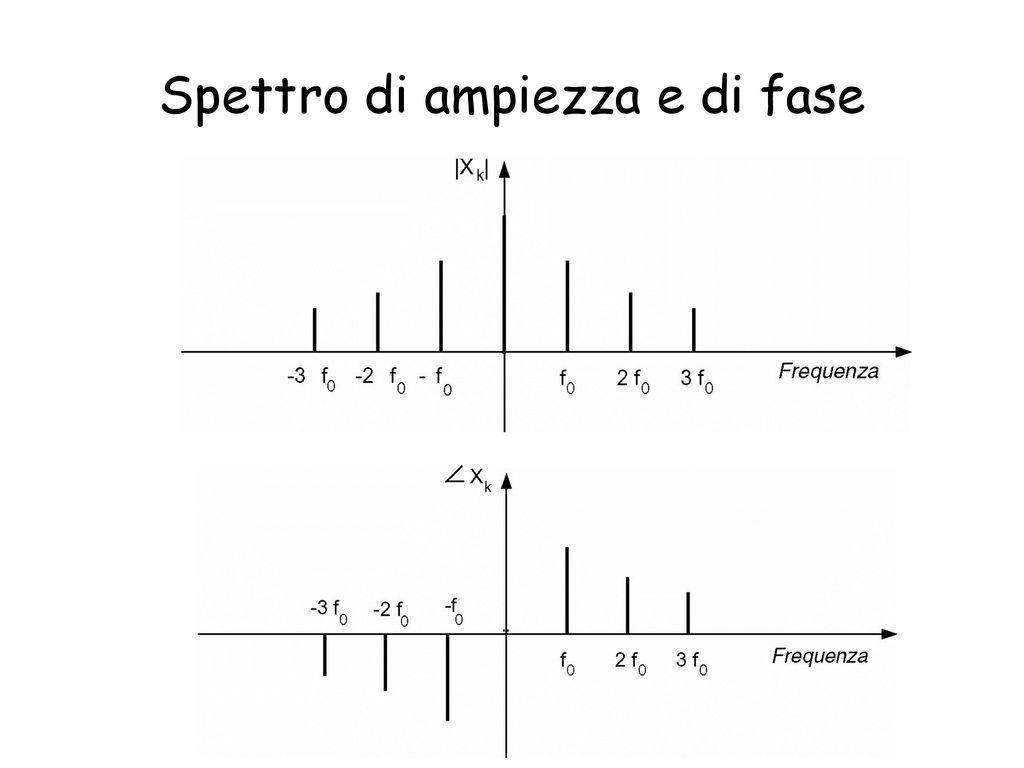
\includegraphics[width=1.0\textwidth]{images/spettro_di_ampiezza_e_di_fase.jpg}
	\caption{Spettro di ampiezza e di fase.}
\end{figure}

%-------------------------------------------------------------------------------
% Subsubsection: Spettro di un coseno
%-------------------------------------------------------------------------------

\subsubsection{Spettro di un coseno}
Consideriamo il segnale
\begin{equation}
	x(t) = A \cos(2 \pi f_0 t).
\end{equation}
Esso rappresenta un'oscillazione cosinusoidale di frequenza $f_0$; il periodo
del segnale \`e $T_0 = 1/f_0$. Ricaviamo i coefficienti di Fourier:
\begin{equation}
	\begin{split}
		X_n = \frac{1}{T_0} \int\displaylimits_{-T_0/2}^{T_0/2} x(t)
		e^{-j 2 \pi n f_0 t} = \frac{1}{T_0}
		\int\displaylimits_{-T_0/2}^{T_0/2} A \cos(2 \pi f_0 t)
		e^{-j 2 \pi n f_0 t} \dt =
		\\
		= \frac{1}{T_0} \int\displaylimits_{-T_0/2}^{T_0/2} A \ 
		\frac{e^{j 2 \pi f_0 t} + e^{-j 2 \pi f_0 t}}{2} \ 
		e^{-j 2 \pi n f_0 t} \dt =
		\quads{6}
		\\
		= \frac{A}{2 T_0} \int\displaylimits_{-T_0/2}^{T_0/2}
		e^{j 2 \pi f_0 (1 - n) t} \dt + \frac{A}{2 T_0} 
		\int\displaylimits_{-T_0/2}^{T_0/2} e^{j 2 \pi f_0 (1 + n) t} 
		\dt =
		\quads{4}
		\\
		= \frac{A}{2 T_0} \int\displaylimits_{-T_0/2}^{T_0/2} \left( 
		\cos[2 \pi f_0 (1 - n) t] + j \sin[2 \pi f_0 (1 - n) t] \right)
		\dt +
		\quads{3}
		\\
		+ \frac{A}{2 T_0} \int\displaylimits_{-T_0/2}^{T_0/2} \left(
		\cos[2 \pi f_0 (1 + n) t] - j \sin[2 \pi f_0 (1 + n) t] \right)
		\dt =
		\quads{3}
		\\
		= \frac{A}{2 T_0} \int\displaylimits_{-T_0/2}^{T_0/2}
		\cos[2 \pi f_0 (1 - n) t] \dt + \frac{A}{2 T_0}
		\int\displaylimits_{-T_0/2}^{T_0/2} j \sin[2 \pi f_0 (1 - n) t]
		\dt +
		\\
		+ \frac{A}{2 T_0} \int\displaylimits_{-T_0/2}^{T_0/2}
		\cos[2 \pi f_0 (1 + n) t] \dt - \frac{A}{2 T_0}
		\int\displaylimits_{-T_0/2}^{T_0/2} j \sin[2 \pi f_0 (1 + n) t]
		\dt =
	\end{split}
\end{equation}
Osserviamo a questo punto che
\begin{equation}
	\begin{split}
		\frac{A}{2 T_0} \int\displaylimits_{-T_0/2}^{T_0/2} \cos[2 \pi f_0 (1 - n) t] \dt =
			\begin{cases}
				\frac{A}{2 T_0} \cdot T_0 = \frac{A}{2} \quad\quad n = 1\\
				\frac{A}{2 T_0} \cdot 0 = 0 \quad\quad \ \ \ n \neq 1
			\end{cases},
		\\
		\frac{A}{2 T_0} \int\displaylimits_{-T_0/2}^{T_0/2} j \sin[2 \pi f_0 (1 - n) t] \dt =
			\begin{cases}
				\frac{A}{2 T_0} \cdot 0 = 0 \quad\quad n = 1\\
				\frac{A}{2 T_0} \cdot 0 = 0 \quad\quad n \neq 1
			\end{cases}
			\quad
	\end{split}
\end{equation}
\begin{equation}
	\begin{split}
		\frac{A}{2 T_0} \int\displaylimits_{-T_0/2}^{T_0/2} \cos[2 \pi f_0 (1 + n) t] \dt =
			\begin{cases}
				\frac{A}{2 T_0} \cdot T_0 = \frac{A}{2} \quad\quad n = -1\\
				\frac{A}{2 T_0} \cdot 0 = 0 \quad\quad \ \ \ n \neq -1
			\end{cases},
		\\
		-\frac{A}{2 T_0} \int\displaylimits_{-T_0/2}^{T_0/2} j \sin[2 \pi f_0 (1 + n) t] \dt =
			\begin{cases}
				-\frac{A}{2 T_0} \cdot 0 = 0 \quad\quad n = -1\\
				-\frac{A}{2 T_0} \cdot 0 = 0 \quad\quad n \neq -1
			\end{cases}
	\end{split}
\end{equation}
Ne segue quindi che
\begin{equation}
	\begin{split}
		= \frac{A}{2 T_0} \int\displaylimits_{-T_0/2}^{T_0/2} 
		\cos[2 \pi f_0 (1 - n) t] \dt + \frac{A}{2 T_0} 
		\int\displaylimits_{-T_0/2}^{T_0/2} j \sin[2 \pi f_0 (1 - n) t] 
		\dt +
		\\
		+ \frac{A}{2 T_0} \int\displaylimits_{-T_0/2}^{T_0/2}
		\cos[2 \pi f_0 (1 + n) t] \dt - \frac{A}{2 T_0}
		\int\displaylimits_{-T_0/2}^{T_0/2} j \sin[2 \pi f_0 (1 + n) t]
		\dt =
		\\
		=
		\begin{cases}
			\frac{A}{2} \quad\quad n = \pm 1\\
			0 \quad\quad \ n \neq \pm 1
		\end{cases}.
		\quads{10}
	\end{split}
\end{equation}
In conclusione,
\begin{equation}
	\begin{split}
		\abs{X_{\pm 1}} = \frac{A}{2} \ ,\\
		\angle X_{\pm 1} = 0.
	\end{split}
\end{equation}
Gli spettri di ampiezza e fase del segnale sono mostrati nella seguente figura:
\begin{figure}[H]
	\centering
	\captionsetup{justification=centering}
	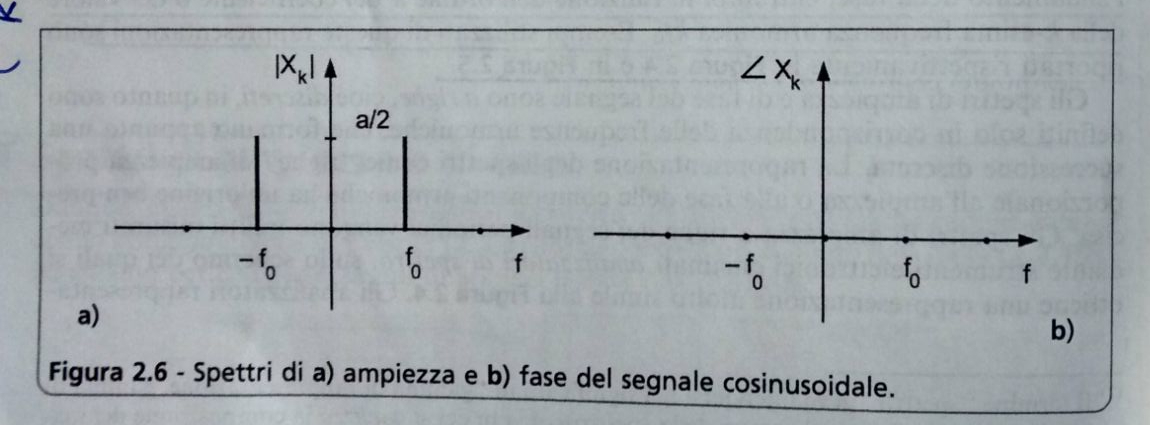
\includegraphics[width=1.0\textwidth]{images/cosine_power_phase_spectrum.jpg}
	\caption{Spettri di ampiezza e fase del segnali cosinusoidale.}
\end{figure}
Il calcolo pu\`o essere effettuato anche tramite un rapido ragionamento: se si
confronta l'espressione in forma polare della serie di Fourier di un segnale
generico
\begin{equation}
	x(t) = A_0 + 2 \sum_{k = 1}^{\infty} A_k
	\cos(2 \pi k f_0 t + \vartheta_k),
\end{equation}
comparandola a
\begin{equation}
	x(t) = A \cos(2 \pi f_0 t).
\end{equation}
\`e possibile vedere immediatamente che
\[
	A_0 = 0
\]
\[
	2 \sum_{k = 1}^{\infty} A_k \cos(2 \pi k f_0 t + \vartheta_k) = A
	\cos(2 \pi f_0 t)
	\footnote{Notare che $\cos(2 \pi f_0 t)$ ha fase iniziale nulla.}
	\Longrightarrow 
		\begin{cases}
			A_1 = \frac{A}{2}, \vartheta_1 = 0\\
			A_k, \vartheta_K = 0 \ \forall k \neq 1
		\end{cases}
\]
ovvero
\[
	X_1 = \frac{A}{2}, X_{-1} = \frac{A}{2};
	\quad X_k = 0 \ \forall k \neq \pm 1.
\]

%-------------------------------------------------------------------------------
% Subsubsection: Spettro di un seno
%-------------------------------------------------------------------------------

\subsubsection{Spettro di un seno}
Consideriamo il segnale
\begin{equation}
	x(t) = A \sin(2 \pi f_0 t).
\end{equation}
Esso rappresenta un'oscillazione sinusoidale di frequenza $f_0$; il periodo del
segnale \`e $T_0 = 1/f_0$. Ricaviamo i coefficienti di Fourier:
\[
	X_n = \frac{1}{T_0} \int\displaylimits_{-T_0/2}^{T_0/2} x(t)
	e^{-j 2 \pi n f_0 t} = \frac{1}{T_0} \int\displaylimits_{-T_0/2}^{T_0/2}
	A \sin(2 \pi f_0 t) e^{-j 2 \pi n f_0 t} \dt =
\]
\[
	= \frac{1}{T_0} \int\displaylimits_{-T_0/2}^{T_0/2} A \ 
	\frac{e^{j 2 \pi f_0 t} - e^{-j 2 \pi f_0 t}}{2j} \ e^{-j 2 \pi n f_0 t}
	\dt =
\]
\[
	= \frac{A}{j 2 T_0} \int\displaylimits_{-T_0/2}^{T_0/2}
	e^{j 2 \pi f_0 (1 - n) t} \dt - \frac{A}{j 2 T_0}
	\int\displaylimits_{-T_0/2}^{T_0/2} e^{j 2 \pi f_0 (1 + n) t} \dt =
\]
\[
	= \frac{A}{j 2 T_0} \int\displaylimits_{-T_0/2}^{T_0/2} \left(
	\cos[2 \pi f_0 (1 - n) t] + j \sin[2 \pi f_0 (1 - n) t] \right) \dt +
\]
\[
	- \frac{A}{j 2 T_0} \int\displaylimits_{-T_0/2}^{T_0/2} \left(
	\cos[2 \pi f_0 (1 + n) t] - j \sin[2 \pi f_0 (1 + n) t] \right) \dt =
\]
\begin{equation}
	\begin{split}
		= \frac{A}{j 2 T_0} \int\displaylimits_{-T_0/2}^{T_0/2}
		\cos[2 \pi f_0 (1 - n) t] \dt + \frac{A}{j 2 T_0}
		\int\displaylimits_{-T_0/2}^{T_0/2} j \sin[2 \pi f_0 (1 - n) t]
		\dt +
		\\
		- \frac{A}{j 2 T_0} \int\displaylimits_{-T_0/2}^{T_0/2}
		\cos[2 \pi f_0 (1 + n) t] \dt + \frac{A}{j 2 T_0}
		\int\displaylimits_{-T_0/2}^{T_0/2} j \sin[2 \pi f_0 (1 + n) t]
		\dt =
	\end{split}
\end{equation}
Osserviamo a questo punto che
\begin{equation}
	\begin{split}
		\frac{A}{j 2 T_0} \int\displaylimits_{-T_0/2}^{T_0/2} \cos[2 \pi f_0 (1 - n) t] \dt =
			\begin{cases}
				\frac{A}{j 2 T_0} \cdot T_0 = \frac{A}{j 2} \quad\quad n = 1\\
				\frac{A}{j 2 T_0} \cdot 0 = 0 \quad\quad \ \ \ n \neq 1
			\end{cases},
		\\
		\frac{A}{j 2 T_0} \int\displaylimits_{-T_0/2}^{T_0/2} j \sin[2 \pi f_0 (1 - n) t] \dt =
			\begin{cases}
				\frac{A}{j 2 T_0} \cdot 0 = 0 \quad\quad n = 1\\
				\frac{A}{j 2 T_0} \cdot 0 = 0 \quad\quad n \neq 1
			\end{cases}
			\quad
	\end{split}
\end{equation}
\begin{equation}
	\begin{split}
		-\frac{A}{j 2 T_0} \int\displaylimits_{-T_0/2}^{T_0/2} \cos[2 \pi f_0 (1 + n) t] \dt =
			\begin{cases}
				-\frac{A}{j 2 T_0} \cdot T_0 = -\frac{A}{j 2} \quad\quad n = -1\\
				-\frac{A}{j 2 T_0} \cdot 0 = 0 \quad\quad \ \ \ \ \ \ n \neq -1
			\end{cases},
		\\
		\frac{A}{j 2 T_0} \int\displaylimits_{-T_0/2}^{T_0/2} j \sin[2 \pi f_0 (1 + n) t] \dt =
			\begin{cases}
				\frac{A}{j 2 T_0} \cdot 0 = 0 \quad\quad n = -1\\
				\frac{A}{j 2 T_0} \cdot 0 = 0 \quad\quad n \neq -1
			\end{cases}
			\quads{2}
	\end{split}
\end{equation}
Ne segue quindi che
\begin{equation}
	\begin{split}
		= \frac{A}{2 T_0} \int\displaylimits_{-T_0/2}^{T_0/2}
		\cos[2 \pi f_0 (1 - n) t] \dt + \frac{A}{2 T_0}
		\int\displaylimits_{-T_0/2}^{T_0/2} j \sin[2 \pi f_0 (1 - n) t]
		\dt +
		\\
		+ \frac{A}{2 T_0} \int\displaylimits_{-T_0/2}^{T_0/2}
		\cos[2 \pi f_0 (1 + n) t] \dt - \frac{A}{2 T_0}
		\int\displaylimits_{-T_0/2}^{T_0/2} j \sin[2 \pi f_0 (1 + n) t]
		\dt =
		\\
		=
		\begin{cases}
			\frac{A}{j 2} \quad\quad \ \ \ \ n = 1\\
			0 \quad\quad \ \ \ \ \ n \neq \pm 1\\
			-\frac{A}{j 2} \quad\quad n = -1
		\end{cases}.
		\quads{10}
	\end{split}
\end{equation}
In conclusione, ricordando che
\[
\frac{A}{j 2} \cdot \frac{j}{j} = -j \cdot \frac{A}{2},
\]
\[
-\frac{A}{j 2} \cdot \frac{j}{j} = j \cdot \frac{A}{2},
\]
possiamo scrivere che
\begin{equation}
	\abs{X_{\pm 1}} = \abs{\pm j \cdot \frac{A}{2}} = \frac{A}{2} \ ,
\end{equation}
\begin{equation}
	\angle X_{\pm 1} =
		\begin{cases}
			\angle -j \cdot \frac{A}{2} = \angle \frac{A}{2} e^{-j}
			= -\frac{\pi}{2}\\
			\angle \ j \cdot \frac{A}{2} = \angle \frac{A}{2} e^{j}
			= \frac{\pi}{2}\\
		\end{cases}.
\end{equation}
Gli spettri di ampiezza e fase del segnale sono mostrati nella seguente
figura:\\
\textbf{Lo spettro di ampiezza \`e ovviamente uguale a quello del coseno visto
precedentemente, mentre lo spettro di fase \`e differente.}
\begin{figure}[H]
	\centering
	\captionsetup{justification=centering}
	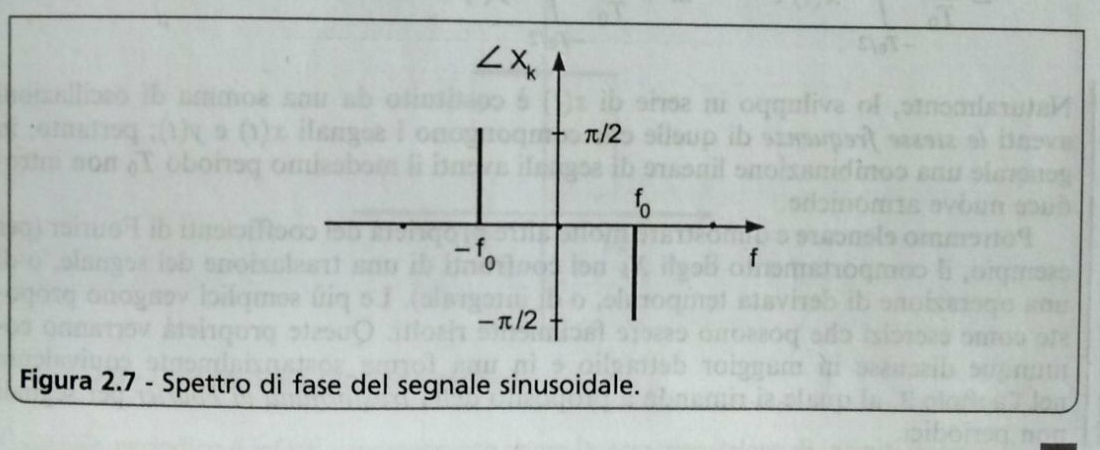
\includegraphics[width=1.0\textwidth]{images/sine_phase_spectrum.jpg}
	\caption{Spettro di fase del segnale sinusoidale.}
\end{figure}
Il calcolo pu\`o essere effettuato anche tramite un rapido ragionamento:
riscriviamo il segnale come
\begin{equation}
	x(t) = A \sin(2 \pi f_0 t) = A \cos(2 \pi f_0 t - \frac{\pi}{2}),
\end{equation}
ora, se si confronta l'espressione in forma polare della serie di Fourier di un
segnale generico
\begin{equation}
	x(t) = A_0 + 2 \sum_{k = 1}^{\infty} A_k
	\cos(2 \pi k f_0 t + \vartheta_k),
\end{equation}
comparandola a
\begin{equation}
	x(t) = A \cos(2 \pi f_0 t - \frac{\pi}{2}).
\end{equation}
\`e possibile vedere immediatamente che
\[
	A_0 = 0
\]
\[
	2 \sum_{k = 1}^{\infty} A_k \cos(2 \pi k f_0 t + \vartheta_k) = A
	\cos(2 \pi f_0 t - \frac{\pi}{2})
	\footnote{Notare che $\cos(2 \pi f_0 t - \frac{\pi}{2})$ ha fase
	iniziale $-\frac{\pi}{2}$.}
	\Longrightarrow 
		\begin{cases}
			A_1 = \frac{A}{2}, \vartheta_1 = -\frac{\pi}{2}\\
			A_k, \vartheta_K = 0 \ \forall k \neq 1
		\end{cases}
\]
ovvero
\[
	X_1 = \frac{A}{2} e^{-j\frac{\pi}{2}}, X_{-1} = \frac{A}{2}
	e^{j\frac{\pi}{2}}; \quad X_k = 0 \ \forall k \neq \pm 1.
\]

%-------------------------------------------------------------------------------
% Subsection: Matlab 2.1
%-------------------------------------------------------------------------------

\newpage
\subsection{MATLAB 2.1}
Verifichiamo le properit\`a della serie di Fourier (simmetria e linearit\`a)
considerando un esempoi di segnale periodico tratto dalla realt\`a. Prendiamo,
in particolare, il tracciato di un \textit{elettrocardiogramma}, che \`e stato
acquisito registrando l'attivit\`a elettrica del cuore di un paziente al variare
del tempo. Come \`e noto, la differenza di potenziale tra gli elettrodi
applicati sul corpo del paziente (cio\`e l'elettrocardiogramma) ha un andamento
tipo (pressoch\'e) periodico, in virtu\`u della regolarit\`a temporale con la
quale vengono prodotti gli impulsi da parte del miocardio.\\
Per verificare sperimentalmente quanto abbiamo appena introdotto, facciamo
ricorso al pacchetto software per l'analisi e la simulazione di segnali Matlab.
Riguardo all'uso di Matlab occorre fare alcune precisazioni: innanzitutto
osserviamo che fino ad ora abbiamo sempre ragionato in termini di segnali
\textit{analogici}, e in particolare di segnali a \textit{tempo continuo}.
Matlab \`e invece un simulatore \textit{a tempo discreto}, che fa uso di segnali
numerici o \textit{digitali}. Questi segnali a tempo discreto vengono introdotti
per \textit{emulare} o \textit{simulare} segnali a tempo continuo (che non
possono essere trattati dai computer digitali). Dunque in luogo di una forma
d'onda continua nel tempo $x(t)$, Matlab elabora un vettore temporale
$\boldsymbol{x}$ ottenuto, come nelle classiche procedure di calcolo numerico,
raccogliendo una successione di \textit{N} valori consecutivi ed equispaziati di
$x(t)$. Tali campioni vengono estratti da $x(t)$ su di un dato intervallo
(dominio) temporale con un certo quanto temporale $\Delta t$; in breve, si ha
che
$\boldsymbol{x} = [x(0), x(\Delta t), x(2 \Delta t), \dots, x((N - 1)\Delta t)]$
. Un vettore $N$-dimensionale come quello appena definito rappresenta la tipica
entit\`a trattata da Matlab per emulare un segnale analogico.
\begin{figure}[H]
	\centering
	\captionsetup{justification=centering}
	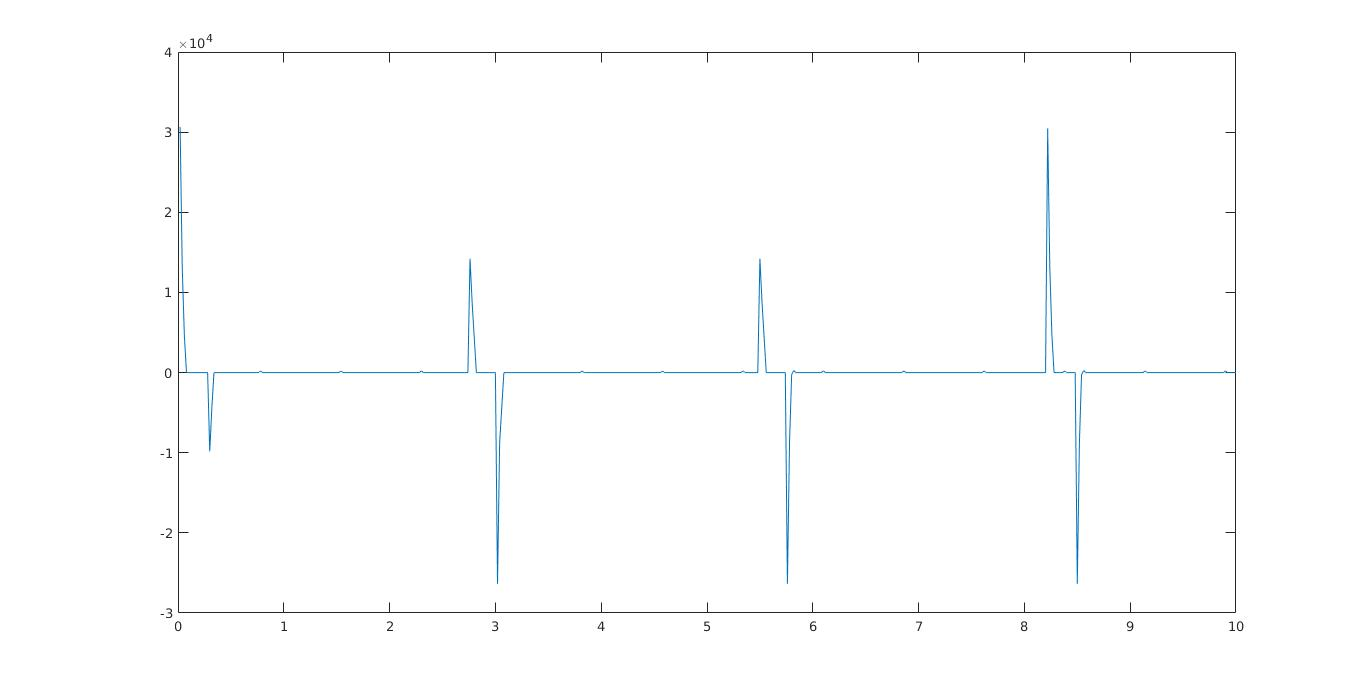
\includegraphics[width=1.0\textwidth]{images/matlab_ecg_signal.jpg}
	\caption{Elettrocardiogramma.}
\end{figure}
La figura precedente riporta l'andamento nel tempo della differenza di
potenziale prodotta dall'attivit\`a cardiaca, registrata su di un paziente
che nel passato ha subito un infarto miocardico (segnali di questo tipo sono
facilmente estraibili da database disponibili online
\footnote{\href{https://www.physionet.org/physiobank/database/mitdb/}{
	https://www.physionet.org/physiobank/database/mitdb/}}).
Nel caso specifico, i dati sono immagazzinati nel file binario 'egc.dat', che
utilizza 16 bit per rappresentare ciascun campione temporale, con una spaziatura
temporale pari a $\Delta t = 20 ms$. Si consideri il seguente script Matlab
\lstinputlisting[frame=single, language=Matlab]{resources/ecg.m}
Le righe di codice
\begin{lstlisting}[frame=single, language=Matlab]
fOut = fopen('ecg.dat');
numeroCampioni = 5000;
x = fread(fOut, numeroCampioni, 'int16');
\end{lstlisting}
servono a leggere $500$ campioni dall'elettrocardiogramma e memorizzarli nel
vettore $\boldsymbol{x}$. A questo punto, \`e possibile visualizzare l'andamento
temporale del segnale con
\begin{lstlisting}[frame=single, language=Matlab]
deltaT = 0.02;
tempo = (1:numeroCampioni)*deltaT;
figure
plot(tempo, x);
\end{lstlisting}
Utilizzando la funzione \texttt{fft} in dotazione a Matlab, \`e possibile
valutare sperimentalmente lo spettro del segnale in esame:
\begin{lstlisting}[frame=single, language=Matlab]
lunghezzaFft = 2^nextpow2(numeroCampioni);
X=fft(x, lunghezzaFft);
X=[X(lunghezzaFft/2+1:lunghezzaFft) X(1:lunghezzaFft/2)];
frequenza = linspace(-0.5, 0.5, length(X))/deltaT;
figure
plot(frequenza, abs(X));
\end{lstlisting}
Il risultato delle precedenti operazioni \`e lo spettro di ampiezza illustrato
di seguito. Come possiamo facilmente vedere, sono presenti righe abbastanza
marcate (e simmetriche rispetto all'origine), che ci consentono di affermare che
lo spettro calcolato \`e quello di un segnale periodico. Possiamo identificare
l'armonica fondamentale $f_0$ a un frequenza praticamente uguale a $1 Hz$; ci\`o
suggerisce che la pulsazione cardiaca del paziente al momento
dell'elettrocardiogramma \`e pari a $60$ battiti al minuto, come del resto ci
potevamo aspettare valutando la distanza temporale $T_0$ tra due picchi
consecutivi del segnale. Tuttavia, lo spettro ottenuto non \`e esattamente a
righe come ci aspetteremo da un segnale periodico: le righe non sono isolate,
in quanto si manifestano componenti frequenziali anche tra un'armonica e
l'altra, e non sono neanche infinitamente strette. Questi fenomeni sono dovuti
al fatto che il battito cardiaco \`e soltanto \textit{approssimativamente}
periodico. In realt\`a anche su piccola scala temporale, l'attivit\`a miocardica
ha leggere irregolarit\`a temporali e quindi lo spettro risultante non \`e
perfettamente a righe.
\begin{figure}[H]
	\centering
	\captionsetup{justification=centering}
	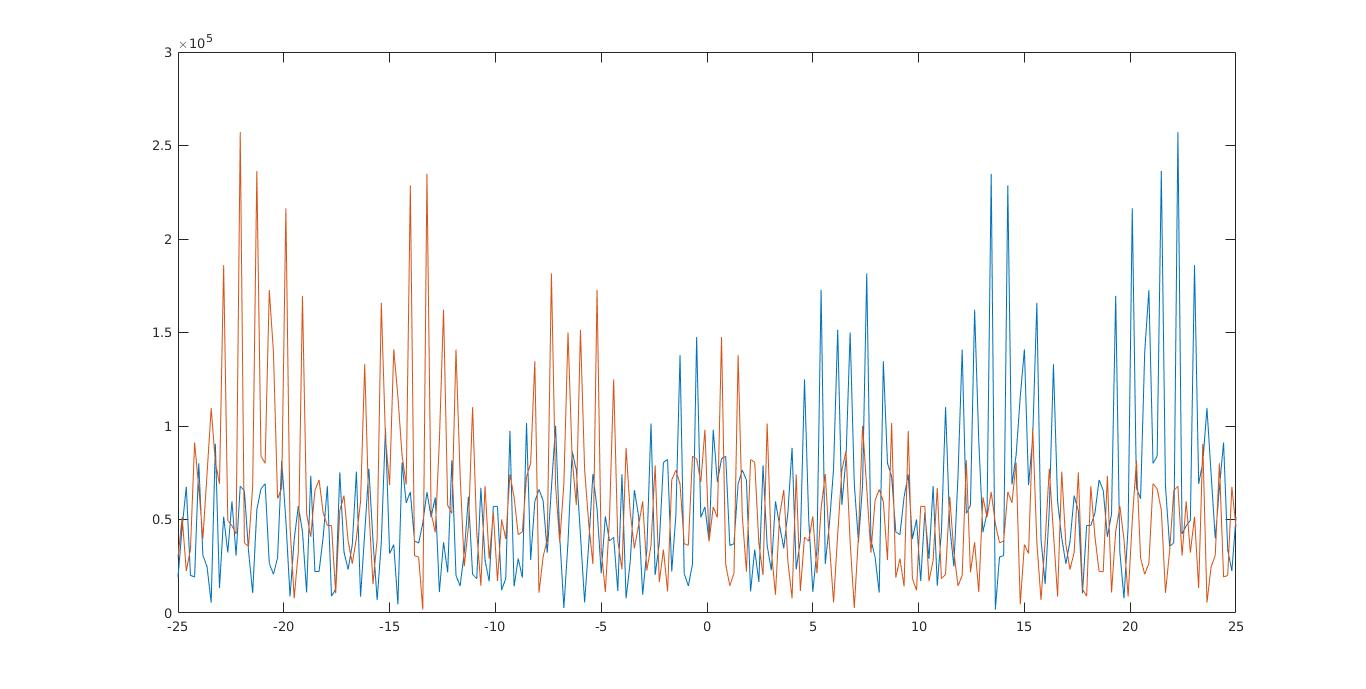
\includegraphics[width=1.0\textwidth]{images/matlab_ecg_spectrum.jpg}
	\caption{Elettrocardiogramma.}
\end{figure}

%-------------------------------------------------------------------------------
% Subsection: Matlab 2.2
%-------------------------------------------------------------------------------

\newpage
\subsection{MATLAB 2.2}
L'equazione di sintesi 
\begin{equation}\label{eq:fourier_series_complex_form}
	x(t) = \sum_{n = -\infty}^{\infty} X_n \ e^{j 2 \pi n f_0 t}
\end{equation}
richiede un numero illimitato di armoniche per ricostruire il segnale periodico
$x(t)$. Le considerazioni fatte per\`o suggeriscono che una approssimazione
soddisfacente del segnale pu\`o essere conseguita anche con un numero
\textit{finito} di armoniche. Possiamo verificare "sperimentalmente" l'effetto
che il troncamento a un numero finito $K$ di armoniche produce sulla sintesi del
segnale \textit{treno di impulsi}
\begin{figure}[H]
	\centering
	\captionsetup{justification=centering}
	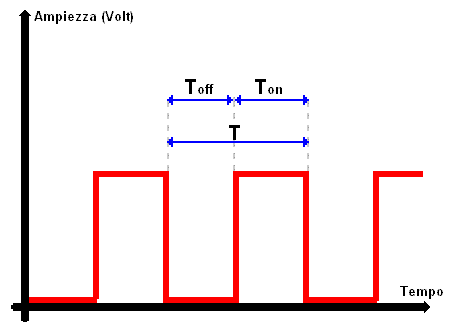
\includegraphics[width=0.5\textwidth]{images/treno_di_impulsi.png}
	\caption{Rappresentazione grafica del segnale treno di impulsi.}
\end{figure}
sfruttando nuovamente il pacchetto software Matlab. Per riprodurre l'equazione
di sintesi dobbiamo generare una rappresentazione vettoriale delle forme d'onda
$cos(2 \pi k f_0 t)$ al variare di $k$. In altre parole, occorre calcolare i
punti di queste curve utilizzando come supporto dei vettori temporali
sufficientemente "fitti" (cio\`e con $\Delta t$ sufficientemente piccolo), che
siano in grado di approssimare in maniera accurata l'andamento dei segnali a
tempo continuo.\\
Si consideri il seguente script Matlab
\lstinputlisting[frame=single, language=Matlab]{resources/fourier_approximation.m}
Di seguito i grafici del seguente script per $K = 3$, $K = 7$, $K = 15$, $K = 30$.
\begin{figure}[H]
	\centering
	\captionsetup{justification=centering}
	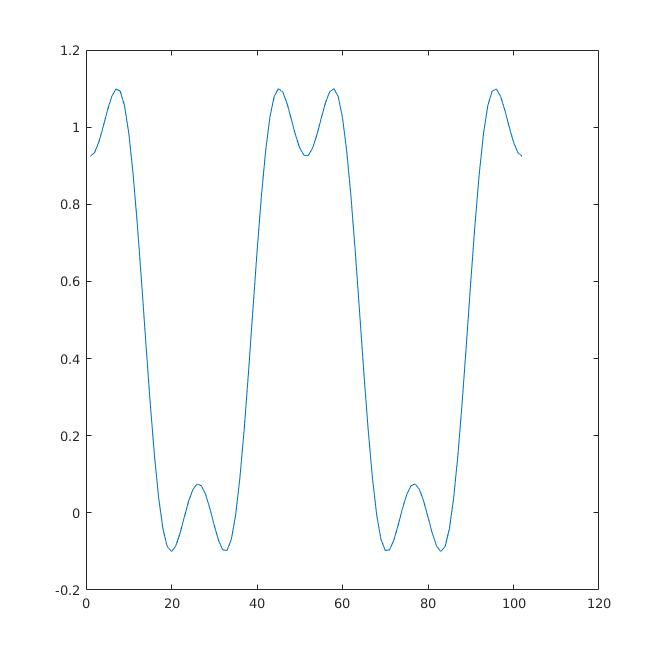
\includegraphics[width=0.5\textwidth]{images/matlab_approssimazione_1.jpg}
	\caption{Approssimazione del treno di impulsi per $K = 3$.}
\end{figure}
\begin{figure}[H]
	\centering
	\captionsetup{justification=centering}
	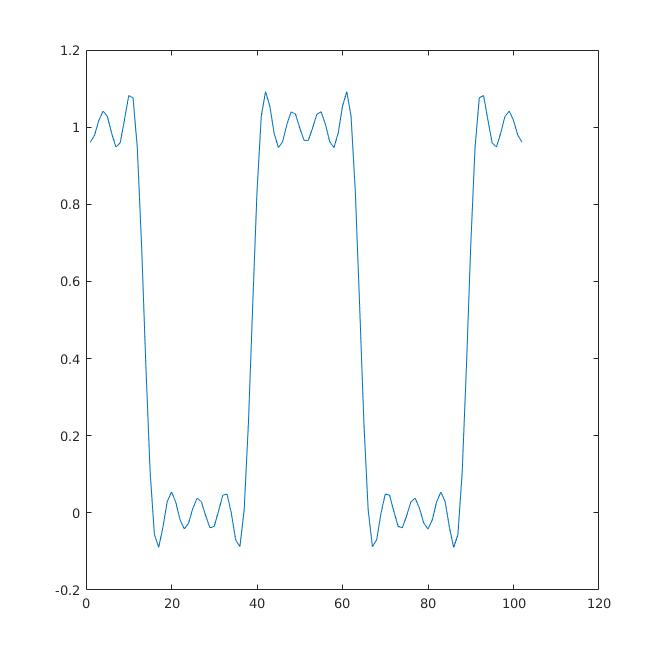
\includegraphics[width=0.5\textwidth]{images/matlab_approssimazione_2.jpg}
	\caption{Approssimazione del treno di impulsi per $K = 7$.}
\end{figure}
\begin{figure}[H]
	\centering
	\captionsetup{justification=centering}
	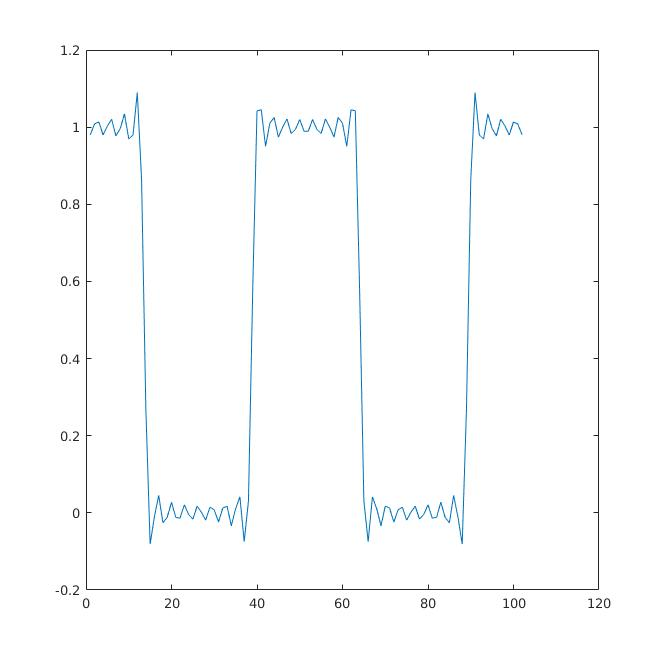
\includegraphics[width=0.5\textwidth]{images/matlab_approssimazione_3.jpg}
	\caption{Approssimazione del treno di impulsi per $K = 15$.}
\end{figure}
\begin{figure}[H]
	\centering
	\captionsetup{justification=centering}
	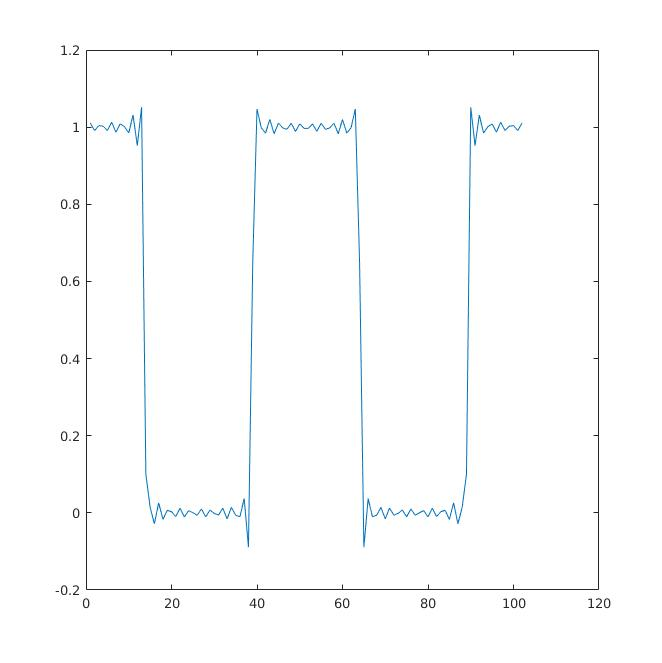
\includegraphics[width=0.5\textwidth]{images/matlab_approssimazione_4.jpg}
	\caption{Approssimazione del treno di impulsi per $K = 30$.}
\end{figure}
\`E interessante fornire la rappresentazione grafica dell'approssimazione che si
ottiene per un valore crescete di $K$ sino ad ottenere una quasi perfetta
rappresentazione del segnale treno di impulsi.
\begin{figure}[H]
	\centering
	\captionsetup{justification=centering}
	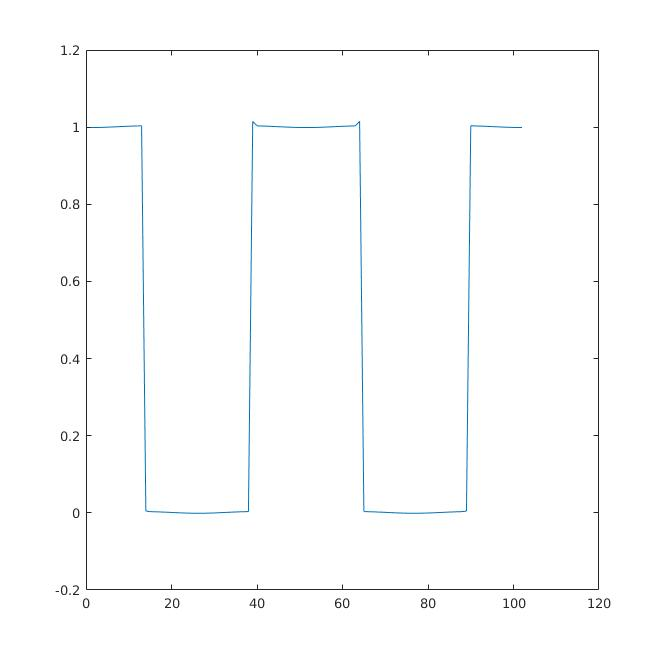
\includegraphics[width=0.5\textwidth]{images/matlab_approssimazione_5.jpg}
	\caption{Approssimazione del treno di impulsi per $K = 300$.}
\end{figure}
\begin{figure}[H]
	\centering
	\captionsetup{justification=centering}
	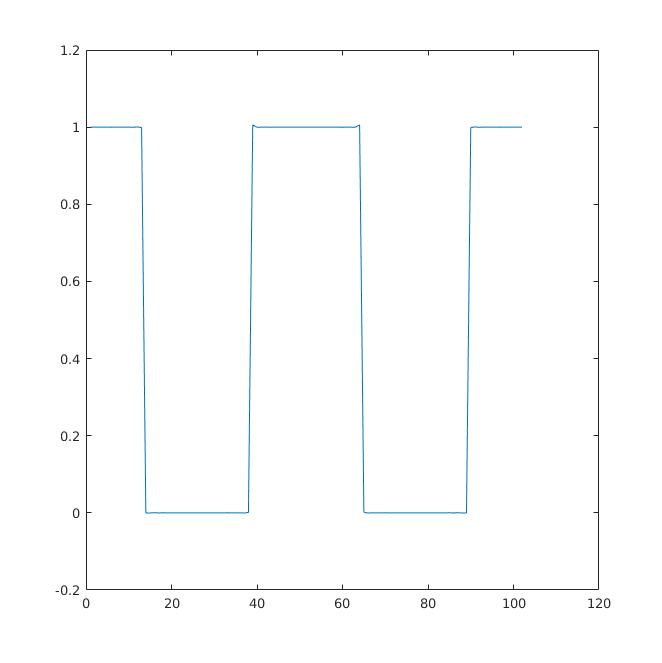
\includegraphics[width=0.5\textwidth]{images/matlab_approssimazione_6.jpg}
	\caption{Approssimazione del treno di impulsi per $K = 3000$.}
\end{figure}
\begin{figure}[H]
	\centering
	\captionsetup{justification=centering}
	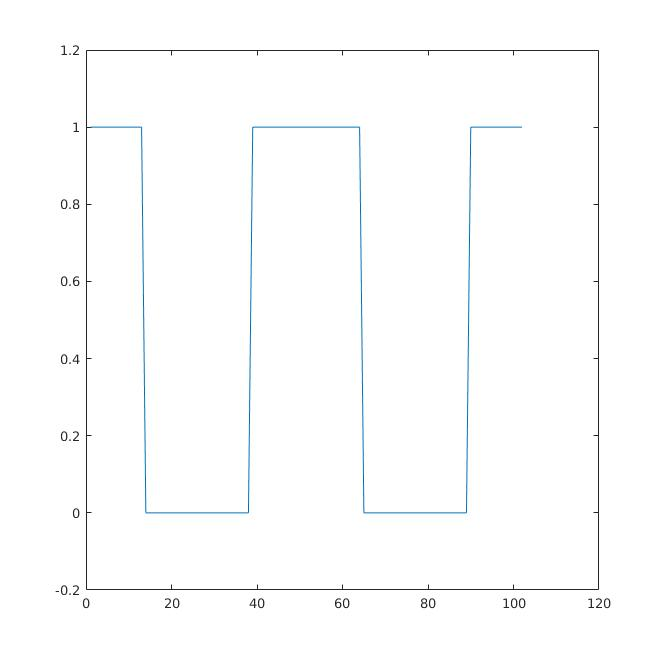
\includegraphics[width=0.5\textwidth]{images/matlab_approssimazione_7.jpg}
	\caption{Approssimazione del treno di impulsi per $K = 30000$.}
\end{figure}
In tutto questo volume gli esperimenti Matlab vengono usati come semplici
strumenti per chiarire ulteriormente i concetti esposti nel testo. Non vi
\`e nessuna pretesa di \textit{far apprendere} Matlab con le sue regole e/o i
suoi trucchi. Non possiamo pre\`o sottrarci, di quando in quando, a qualche
osservazione di carattere generale sulla programmazione. In particolare, il
codice presentato qui sopra merita alcune precisazioni riguardo allo stile di
scrittura. Come \`e possibile notare soprattutto nelle ultime righe, l'approccio
adottato fa un uso apprezzabile di \textit{matrici} e \textit{vettori}, a
scapito talvolta della leggibilit\`a del codice. Per esempio, invece di
utilizzare un ciclo \texttt{for} in funzione dei coefficienti \texttt{k} per
l'equazione di sintesi come in
\begin{lstlisting}[frame=single, language=Matlab]
% X_0 = 1/2
componenteContinua = 0.5;

% inizializzazione del vettore del segnale approssimante
ones(1, length(tempoNormalizzato));

% ciclo sui vari indici k
for k = 1:2:K
	% X_k
	coefficienteK = 2/(k*pi)*(-1)^((k-1)/2);
	
	% aggiornamento del vettore segnale approssimante mediante l'equazione di sintesi
	xApprossimante = xApprossimante + coefficienteK * cos(2*pi*k*tempoNormalizzato);
end
\end{lstlisting}
(e come si farebbe utilizzando un linguaggio di programmazione general-purpose,
per esempio C o C++), abbiamo usato il prodotto matriciale tra vettore
\texttt{coseni} e \texttt{coefficienti}. Il motivo di tale scelta risiede nel
fatto che Matlab, a differenza di altri ambienti di simulazione numerica e altri
linguaggi di programmazione, \`e ottimizzato per il calcolo matriciale. \`E
buona regola, quindi, sfruttare questa caratteristica, adottando uno stile di
programmazione conseguente, per ottenere un codice efficiente che venga eseguito
velocemente sulla piattaforma di calcolo utilizzata.

%-------------------------------------------------------------------------------
% Section: Segnali aperiodici a tempo continuo
%-------------------------------------------------------------------------------

\newpage
\section{Segnali aperiodici a tempo continuo}
Consideriamo il segnale detto \textit{treno di impulsi rettangolari di durata
$T$ e periodo $T_0$} ($T < T_0$) rappresentato nella seguente figura
\begin{figure}[H]
	\centering
	\captionsetup{justification=centering}
	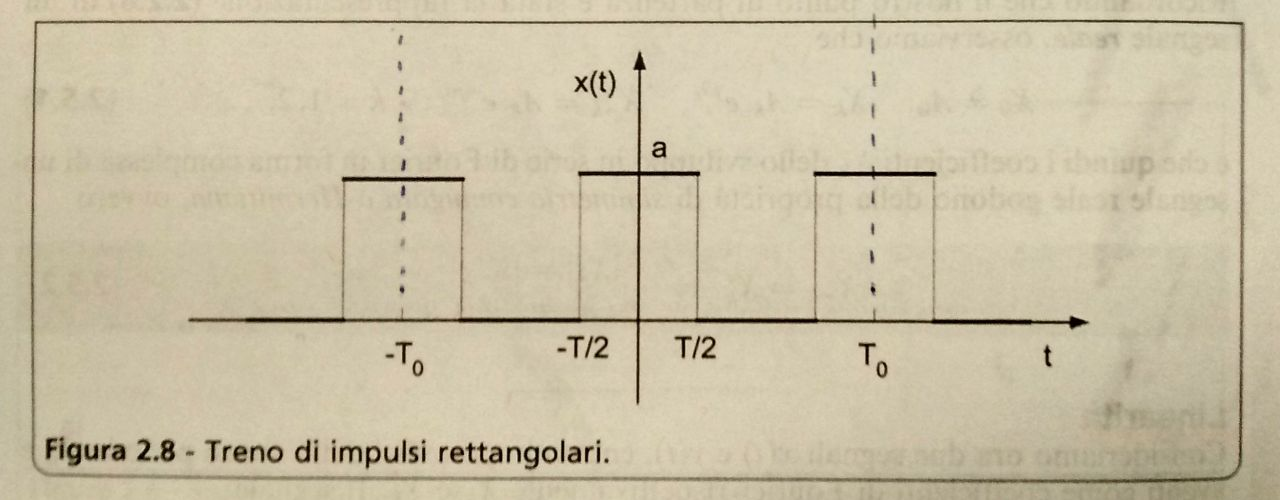
\includegraphics[width=1.0\textwidth]{images/treno_di_impulsi_rettangolari.jpg}
	\caption{Treno di impulsi rettangolari.}
\end{figure}
Per questo segnale si definisce il parametro \textit{duty-factor} (o 
\textit{duty-cycle}) $\delta = T/T_0$ che esprime il rapporto tra la durata $T$
di ciascun impulso e il periodo di ripetizione del segnale $T_0$.
\bigbreak
Per rappresentare pi\`u comodamente il treno di impulsi rettangolari \`e utile
definire la funzione
\begin{equation}
	rect(\alpha) \triangleq
		\begin{cases}
			1 \quad\quad \abs{\alpha} < \frac{1}{2}\\
			\frac{1}{2} \quad\quad \abs{\alpha} = \frac{1}{2}\\
			0 \quad\quad altrove
		\end{cases}
\end{equation}
il cui andamento (impulso rettangolare) \`e rappresentato nella seguente figura
\begin{figure}[H]
	\centering
	\captionsetup{justification=centering}
	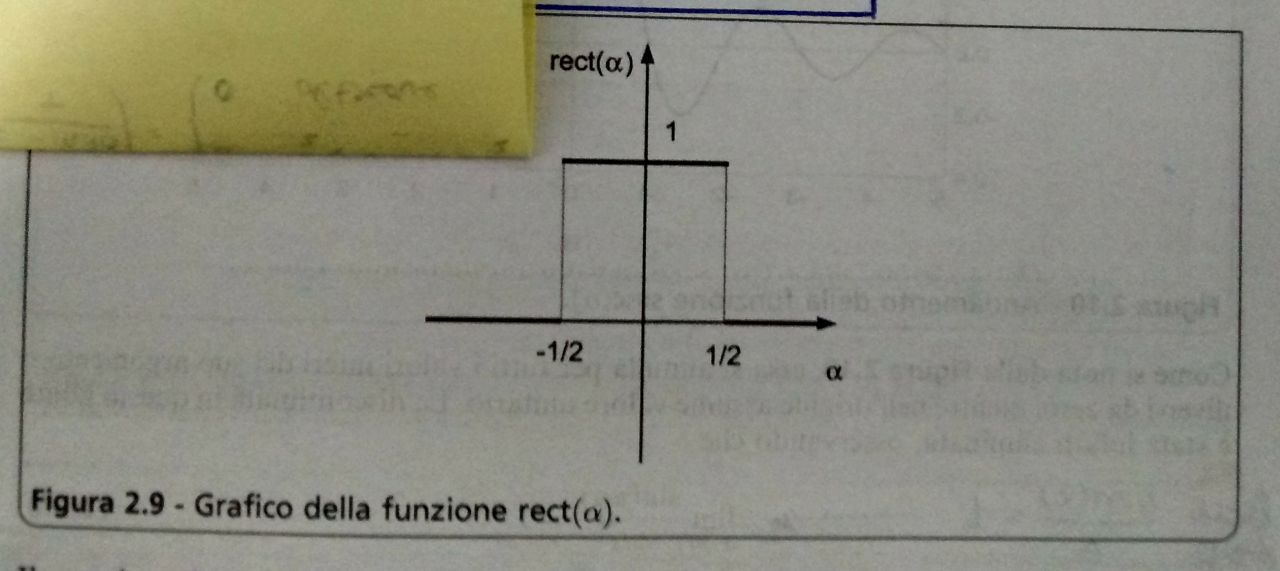
\includegraphics[width=1.0\textwidth]{images/rect_alpha.jpg}
	\caption{Grafico della funzione $rect(\alpha)$.}
\end{figure}
Ancora una volta, questa semplice funzione rappresenta un'astrazione matematica
utile per schematizzare impulsi che hanno \textit{tempo di salita} molto breve
rispetto alla propria \textit{durata}. Utilizzando questa funzione \`e possibile
scrivere la seguente espressione per il treno di impulsi rettangolari
\begin{equation}
	x(t) = \sum_{n = -\infty}^{+\infty} a \cdot rect\left(\frac{t - nT_0}{T}
	\right).
\end{equation}
Il segnale periodico \textit{treno di impulsi rettangolari} \`e infatti
rappresentato come la \textit{sovrapposizione} di infiniti impulsi di durata $T$
ottenuti ciascuno \textit{ritardando} l'impulso "base" non periodico $rect(t/T)$
di $nT_0$ secondi con $n = 0, \pm1,\dots$. In questo caso diremo che
l'impulso-base $rect(t/T)$ \`e stato \textit{periodicizzato} con periodo di
ripetizione $T_0$ per ottenere il segnale $x(t)$.
\bigbreak
Calcoliamo ora i coefficienti dello sviluppo in serie del segnale in esame:
\[
	X_n = \frac{1}{T_0} \int\displaylimits_{-T_0/2}^{T_0/2} x(t)
	e^{-j 2 \pi n f_0 t} \dt =\footnote{Calcolare il coefficiente per
	$rect(t/T)$ \`e equivalente a calcolarlo per
	$rect\left(\frac{t - nT_0}{T}\right)$ dato che la funzione \`e
	periodica.} \frac{1}{T_0} \int\displaylimits_{-T_0/2}^{T_0/2} a 
	\cdot rect(t/T) e^{-j 2 \pi n f_0 t} \dt =
\]
\begin{equation}
	\begin{split}
		= \underbrace{\frac{1}{T_0} \int\displaylimits_{-T/2}^{T/2} a
		\cdot e^{-j 2 \pi n f_0 t} \dt}_{rect(t/T) \ = \ 1 \ \forall \ 
		t \ \in \ [-T/2, \ T/2]} = \frac{1}{T_0}
		\int\displaylimits_{-T/2}^{T/2} a \cdot
		\frac{-j 2 \pi n f_0}{-j 2 \pi n f_0} \cdot e^{-j 2 \pi n f_0 t}
		\dt =
		\\
		= \frac{a}{T_0} \cdot \frac{1}{-j 2 \pi n f_0}
		\int\displaylimits_{-T/2}^{T/2} (-j 2 \pi n f_0) \cdot
		e^{-j 2 \pi n f_0 t} \dt =
		\quads{4}
		\\
		= \frac{a}{T_0} \cdot \left[
			\frac{e^{-j 2 \pi n f_0 t}}{(-j 2 \pi n f_0)}
		\right]_{-T/2}^{T/2} = \frac{a}{T_0} \cdot
		\frac{e^{-j 2 \pi n f_0 t} - e^{j 2 \pi n f_0 t}}{(-j 2 \pi n f_0)} =
		\quads{3}
		\\
		= \frac{a}{T_0} \frac{e^{-j 2 \pi n f_0 t} - e^{j 2 \pi n f_0 t}}{(-j 2 \pi n f_0)}
		= \frac{a}{T_0} \frac{sin(\pi n f_0 T}{\pi n / T_0} =
		\quads{4}
		\\
		= \frac{a T}{T_0} \cdot \frac{sin(\pi n T/T_0)}{\pi n T/T_0}
		\quads{9}
		\\
	\end{split}
\end{equation}
Per esprimere $X_n$ in una forma pi\`u concisa, definiamo una ulteriore funzione
notevole
\begin{equation}
	sinc(\alpha) \triangleq \frac{sin(\pi \alpha)}{\pi \alpha},
\end{equation}
per cui
\begin{equation}
	X_n = \frac{aT}{T_0} sinc(\frac{kT}{T_0}) = a \ \delta \ sinc(k \delta),
\end{equation}
dove si \`e posto $\delta = T/T_0$ e $\alpha = kT/T_0$.

%-------------------------------------------------------------------------------
% Subsection: Dalla serie all'integrale di Fourier
%-------------------------------------------------------------------------------

\subsection{Dalla serie all'integrale di Fourier}
Il significato e l'importanza della rappresentazione in serie di Fourier di un
segnale periodico a tempo continuo sono stati ampiamente discussi nella sezione
precedente. Molti segnali che si osservano nei fenomeni naturali non sono per\`o
periodici. Sorge allora immediata la questione della possibilit\`a di ottenere
una scomposizione simile alla serie di Fourier \textit{anche per i segnali
aperiodici}. \textbf{\`E possibile cio\`e rappresentare anche un segnale non
periodico come una opportuna \textit{sovrapposizione} di segnali elementari, in
particolare sinusoidali?}
\bigbreak
Per rispondere a questa domanda, consideriamo come caso di studio il segnale
aperiodico appena introdotto impulso rettangolare:
\[
	x(t) = rect\left(\frac{t}{T}\right).
\]
Mettiamo ora in relazione questo segnale con il treno di impulsi rettangolari
\textit{periodico}
\begin{equation}
	x_p(t) = \sum_{n = -\infty}^{+\infty} x(t - nT_0) =
	\sum_{n = -\infty}^{+\infty} rect\left(\frac{t - nT_0}{T}\right)
\end{equation}
di cui gi\`a conosciamo la rappresentazione in serie di Fourier. Come \`e chiaro
, $x_p(t)$ \`e ottenuto \textit{periodicizzando} $x(t)$ con periodo di
ripetizione $T_0$, come suggerito nella seguente figura
\begin{figure}[H]
	\centering
	\captionsetup{justification=centering}
	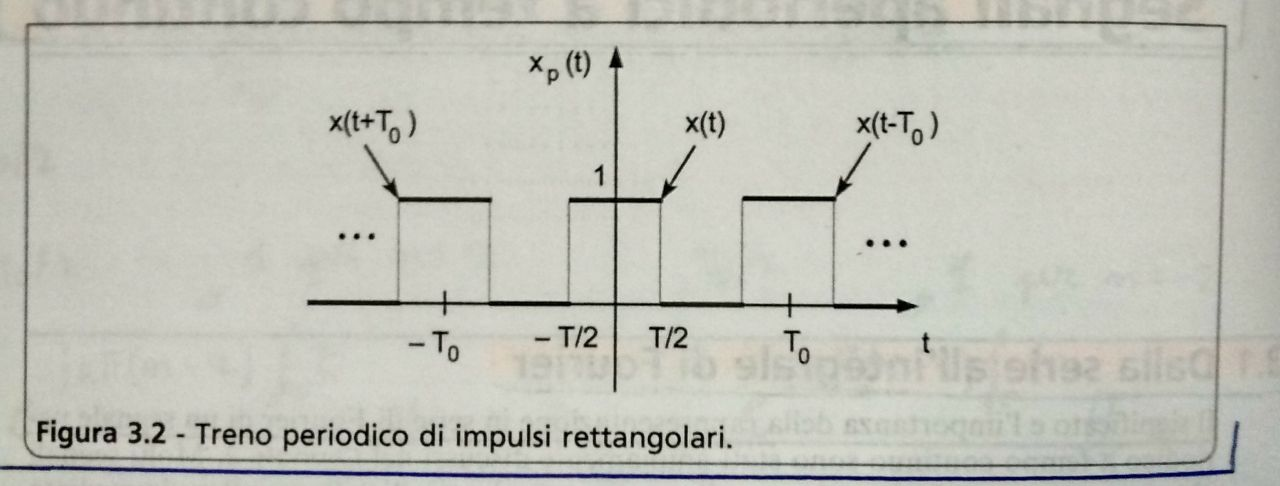
\includegraphics[width=1.0\textwidth]{images/treno_di_impulsi_rettangolari_2.jpg}
	\caption{Treno di impulsi rettangolari.}
\end{figure}
Il segnale originario $x(t)$ pu\`o essere considerato come una sorta di
caso-limite di un segnale periodico: partendo da $x_p(t)$, si riottiene
l'impulso "base" $x(t)$ centrato in $t = 0$ se si pensa di \textit{fare una
periodicizzazione di periodo $T_0 \rightarrow \infty$}. Al di l\`a del
particolare esempio, se si costruisce un segnale periodico $x_p(t)$ per
periodicizzazione del segnale aperiodico $x(t)$ \`e vero in generale che
\begin{equation}
	x(t) = \lim_{T_0 \rightarrow \infty} x_p(t).
\end{equation}
Naturalmente, il segnale $x_p(t)$, essendo periodico di periodo $T_0$, pu\`o
essere rappresentato mediante serie di Fourier tramite la ben nota relazione
\[
	x_p(t) = \sum_{n = -\infty}^{+\infty} X_n e^{j 2 \pi n f_0 t}
\]
con $f_0 = 1/T_0$ e con i coefficienti di Fourier $X_n$ dati da
\[
	X_n = \frac{1}{T_0} \int\displaylimits_{-T_0/2}^{T_0/2} x_p(t)
	e^{-j 2 \pi n f_0 t} \dt.
\]
\textbf{Questo ci fa gi\`a intuire che, dato che il segnale $x(t)$ rappresenta
un caso limite del segnale $x(t)$, sia possibile ottenere una espressione
tramite i coefficienti di Fourier anche per il segnale aperiodico $x(t)$ come
caso limite dei coefficienti di Fourier del segnale periodico $x_p(t)$.}
\bigbreak
Nase adesso l'esigenza di stabilire il comportamento della serie di Fourier e
dei relativi coefficienti $X_n$ quando $T_0 \rightarrow \infty$.\\
Osserviamo innanzitutto che aumentando il periodo di ripetizione $T_0$ si riduce
la frequenza fondamentale $f_0 = 1/T_0$, e quindi si riduce la differenza tra due
generiche frequenze armoniche consecutive. Ci\`o determina un infittimento dello
spettro del segnale se la scala di rappresentazione delle frequenze resta la
stessa. Inoltre, dalla relazione 
\[
	X_n = \frac{1}{T_0} \int\displaylimits_{-T_0/2}^{T_0/2} x_p(t)
	e^{-j 2 \pi n f_0 t} \dt
\]
\`e facile vedere che l'\textit{ampiezza} dei coefficienti tende a ridursi man
mano che $T_0$ cresce; al limite, per $T_0 \rightarrow \infty$, lo spettro di
$x_p(t)$ tende a divenire sempre pi\`u fitto e ad assumere valori sempre pi\`u
piccoli per tutte le frequenze armoniche.\\
Si pu\`o facilmente ovviare al problema della riduzione delle ampiezze delle
righe spettrali definendo, per ciascuna delle frequenze armoniche $nf_0$, una
sorta di "coefficiente di Fourier modificato"
\begin{equation}
	X(nf_0) \triangleq T_0 \cdot X_n = \int\displaylimits_{-T_0/2}^{T_0/2}
	x_p(t) e^{-j 2 \pi n f_0 t} \dt
\end{equation}
che evidentemente non \`e una quantit\`a che tende a zero per
$T_0 \rightarrow \infty$.\\
Riscriviamo dunque l'espansione in serie di Fourier di $x_p(t)$ usando il
coefficiente modificato\footnote{Dato che si \`e posto
$X(nf_0) \triangleq T_0 \cdot X_n$, ne segue che
$X_n = X(n f_0) \frac{1}{T_0} = X(n f_0) \cdot f_0$.}
\begin{equation}
	x_p(t) = \sum_{n = -\infty}^{+\infty} X(n f_0) e^{j 2 \pi n f_0 t}
	\cdot f_0.
\end{equation}
Possiamo adesso effettuare il passaggio cruciale al limite per
$T_0 \rightarrow \infty$ (ovvero per $f_0 \rightarrow 0$. Il segnale periodico
$x_p(t)$ al primo membro si trasforma nel segnale aperiodico $x(t)$. La somma a
secondo membro invece, per definizione, si trasforma in un \textit{integrale} e
si ottiene uno \textit{sviluppo} del segnale aperiodico $x(t)$ tramite
\begin{equation}\label{eq:fourier_integral}
	x(t) = \int\displaylimits_{-\infty}^{+\infty} X(f) e^{j 2 \pi f t} \df.
\end{equation}
Il segnale aperiodico \`e dunque rappresentabile attraverso il cosiddetto
\textbf{integrale di Fourier}. Resta da determinare l'espressione della funzione
$X(f)$ che compare nell'integrando della \eqref{eq:fourier_integral}.
Innanzitutto, \`e chiaro che tale quantit\`a risulta una funzione complessa
della variabile continua $f$, che mantiene il significato di \textit{frequenza}.
L'espressione di $X(f)$ si ottiene passando al limite per
$T_0 \rightarrow \infty$ nella definizione di $X(nf_0)$ del coefficiente di
Fourier modificato:
\begin{equation}\label{eq:tcf_coefficient}
	X(f) = \lim_{\begin{split}T_0 \rightarrow \infty \\ f_0 \rightarrow 0\end{split}}
		\int\displaylimits_{-T_0/2}^{T_0/2} x_p(t) e^{-j 2 \pi n f_0 t}
		\dt = \int\displaylimits_{-\infty}^{\infty} x(t)
		e^{-j 2 \pi n f t} \dt 
\end{equation}
che rappresenta la \textbf{trasformata continua di Fourier del segnale $x(t)$}.\\
In maniera euristica, possiamo dire che la variabile continua $f$ \`e, in un
certo senso, il limite della variabile discreta $n f_0$ di partenza, quando
$f_0 \rightarrow 0$.
\bigbreak
\textbf{Commentiamo il risultato ottenuto.} Nella serie di Fourier per un
segnale periodico, quest'ultimo viene rappresentato mediante componenti
sinusoidali a frequenze in \textit{relazione armonica}, cio\`e tutti multiple di
un'unica fondamentale, nonch\`e di ampiezza \textit{finita}. Nel caso del
segnale aperiodico, la \eqref{eq:fourier_integral}, detta anche
\textit{antitrasformata di Fourier} (o \textit{trasformata inversa di Fourier}),
permette ancora di rappresentare il segnale aperiodico $x(t)$ come la
sovrapposizione di componenti sinusoidali, ma questa volta di ampiezza
\textit{infinitesima} $\abs{X(f)} \df$ e di frequenza $f$ variabile \textit{con
continuit\`a} su tutto l'asse reale. In altre parole, il segnale aperiodico \`e
visto come un segnale periodico "di periodo illimitato" e quindi con frequenza
fondamentale "infinitamente piccola".
\bigbreak
Riportiamo di nuovo le due equazioni relative alla rappresentazione del segnale
aperiodico, osservando che in generale indicheremo con la lettera maiuscola $X$,
$Y$, $Z$, la trasformata di Fourier rispettivamente di un segnale $x$, $y$, $z$:
\begin{equation}
	x(t) = \int\displaylimits_{-\infty}^{\infty} X(f) e^{j 2 \pi f t} \df
	\quad\quad , \quad\quad X(f) =
	\int\displaylimits_{-\infty}^{\infty} x(t) e^{-j 2 \pi f t} dt.
\end{equation}
La prima delle due rappresenta evidentemente un'equazione di \textit{sintesi}
che permette di rappresentale il segnale come sovrapposizione di segnali
elementari, ed \`e chiaramente analoga alla
\eqref{eq:fourier_series_complex_form} per i segnali periodici; la seconda \`e
un'equazione di \textit{analisi}, analoga alla \eqref{eq:fourier_coefficient},
che permette di determinare il \textit{peso} che le varie componenti
frequenziali (a tutte le possibili frequenze variabili con continuit\`a da
$-\infty$ a $+\infty$). hanno nella composizione di $x(t)$. Tali relazioni
mettono in corrispondenza un segnale del tempo con la propria trasformata di
Fourier, funzione a valori complessi della frequenza. Come d'uso anche con i
coefficienti di Fourier, questa relazione viene riassunta con la notazione
\begin{equation}
	x(t) \iff X(f).
\end{equation}
Un modo alternativo di indicare sinteticamente le operazioni di trasformata e
antitrasformata \`e quello mutuato alla notazione degli operatori caratteristica
dell'analisi funzione:
\begin{equation}
	X(f) = \mathcal{F}[x(t)] \quads{2} , \quads{2} x(t) =
	\mathcal{F}^{-1}[X(f)]
\end{equation}

%-------------------------------------------------------------------------------
% Subsubsection: Esempio
%-------------------------------------------------------------------------------

\subsubsection{Esempio}
Conseideriamo il segnale impulso rettangolare
\[
	x(t) = rect\left(\frac{t}{T}\right)
\]
e calcoliamone la trasformata di Fourier $X(f)$. questa \`e data da
\[
	X(f) = \int\displaylimits_{-\infty}^{+\infty} x(t) e^{-j 2 \pi f t} \dt
	= \int\displaylimits_{-\infty}^{+\infty} rect\left(\frac{t}{T}\right)
	e^{-j 2 \pi f t} \dt =
\]
\[
	= \int\displaylimits_{-T/2}^{T/2} rect\left(\frac{t}{T}\right)
	e^{-j 2 \pi f t} \dt = \int\displaylimits_{-T/2}^{T/2} 1 \cdot
	e^{-j 2 \pi f t} \dt =
\]
\[
	= \left[\frac{e^{-j 2 \pi f t}}{-j 2 \pi f}\right]_{-T/2}^{T/2} =
	\frac{\sin(\pi f T)}{\pi f}.
\]
Gli spettri di ampiezza e di fase del segnale $x(t)$ sono rappresentati nella
seguente figura
\begin{figure}[H]
	\centering
	\captionsetup{justification=centering}
	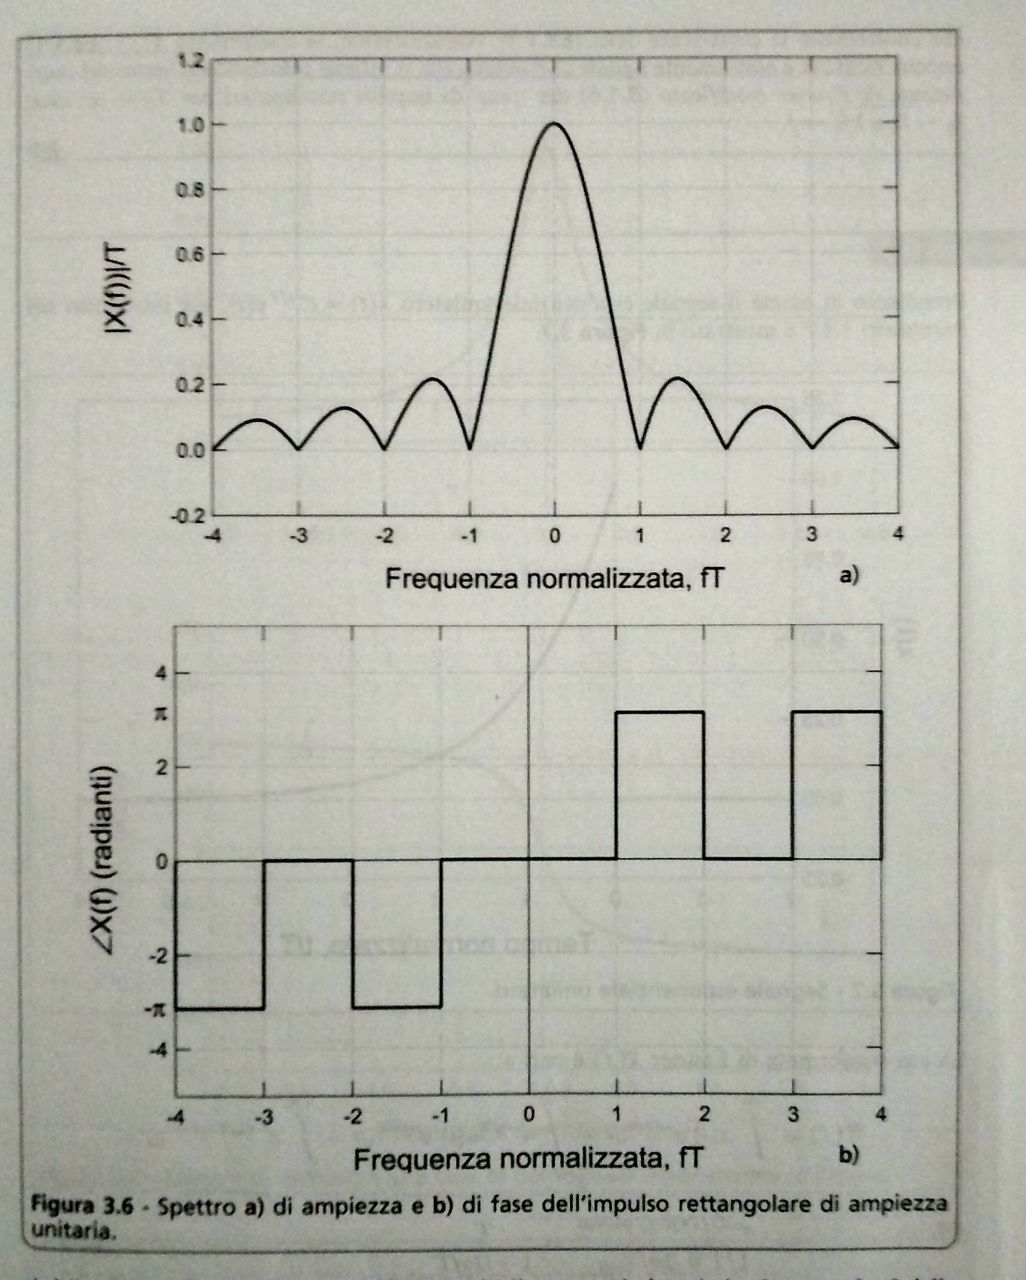
\includegraphics[width=1.0\textwidth]{images/spettro_rect_alpha.jpg}
	\caption{Spetro \textbf{a)} di ampiezza e \textbf{b)} di fase
		dell'impulso rettangolare di ampiezza unitaria.}
\end{figure}

%-------------------------------------------------------------------------------
% Subsubsection: Esempio
%-------------------------------------------------------------------------------

\subsubsection{Esempio}
Consideriamo il segnale
\[
	x(t) = 2 \cdot rect\left(\frac{t}{2T}\right) +
	1 \cdot rect\left(\frac{t}{T}\right)
\]
graficamente rappresentabile come
\begin{figure}[H]
	\centering
	\captionsetup{justification=centering}
	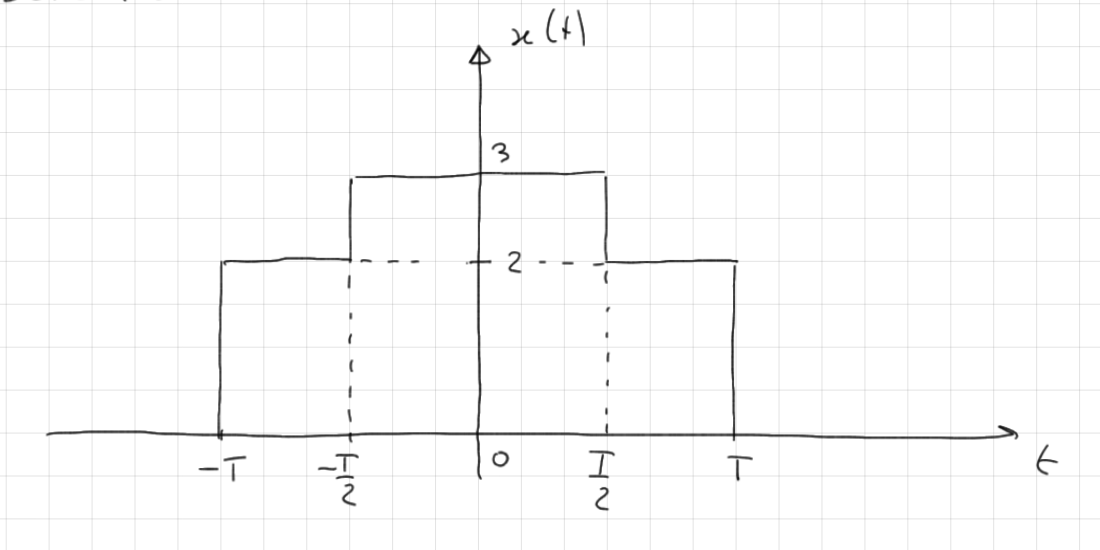
\includegraphics[width=1.0\textwidth]{images/esempio_14_03_2018.png}
	\caption{Segnale $x(t)$.}
\end{figure}
\noindent
Possiamo scomporre il nostro segnale come constributo di due segnali
\[
	x_1(t) = 2 \cdot rect\left(\frac{t}{2T}\right)
\]
\[
	x_2(t) = 1 \cdot rect\left(\frac{t}{T}\right)
\]
Calcoliamone la trasformata di Fourier.
\bigbreak\noindent
Sappiamo gi\`a che 
\[
	X_2(f) = T \cdot sinc(f T).
\]
Calcoliamo quindi la trasformata di $x_1(t)$
\[
	x_1(t) = 2 \cdot rect\left(\frac{t}{2T}\right) =
	2 \cdot rect\left(\frac{t}{T'}\right)
\]
da cui segue immediatamente che
\[
	X_1(f) = 2 \cdot T' \cdot sinc(f T') =
	2 \cdot 2T \cdot sinc(f 2T) =
	4T \cdot sinc(2 f T).
\]
Infine
\[
	X(f) = X_1(f) + X_2(f) =
	4T \cdot sinc(2 f T) + T \cdot sinc(f T).
\]

%-------------------------------------------------------------------------------
% Subsubsection: Esempio
%-------------------------------------------------------------------------------

\subsubsection{Esempio}
Consideriamo il segnale
\[
	x(t) = A \cdot rect\left(\frac{t - 3T}{T}\right)
\]
Graficamente rappresentabile come
\begin{figure}[H]
	\centering
	\captionsetup{justification=centering}
	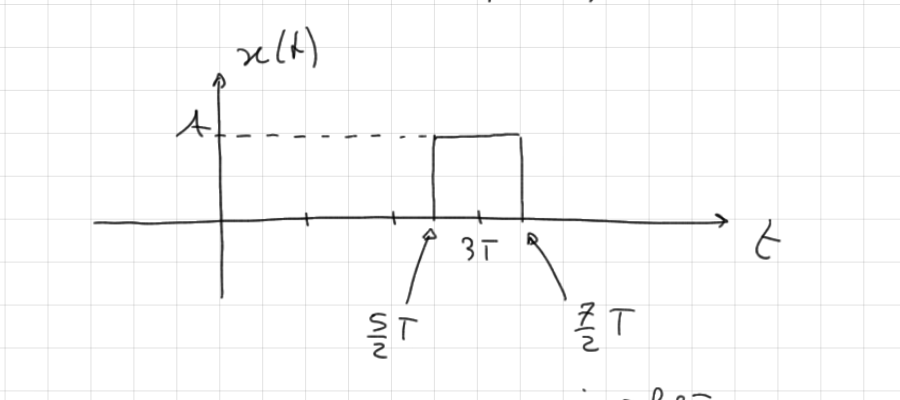
\includegraphics[width=1.0\textwidth]{images/esempio_14_03_2018_2.png}
	\caption{Segnale $x(t)$.}
\end{figure}
Per calcolarne la trasformata continua possiamo utilizzare il \textbf{teorema
del ritardo}.
\[
	X(f) = A \cdot T sinc(f T) \cdot e^{-j 2 \pi f 3T}.
\]

%------------------------------------------------
% Subsubsection: Esempio
%------------------------------------------------

\newpage
\subsection{Criteri di esistenza della Trasformata Continua di Fourier (TCF)}
Indichiamo adesso delle condizioni sufficienti per la rappresentazione del
segnale $x(t)$ attraverso la propria trasformata di Fourier $X(f)$, nel senso
gi\`a discusso riguardo la serie di Fourier. Se tali condizioni sono soddisfatte
\`e possibile affermare che la conoscenza dell'andamento nel tempo del segnale
$x(t)$ \`e equivalente alla conoscenza dell'andamento frequenziale della
relativa trasformata di Fourier.\\
Una prima condizione sufficiente afferma che se il segnale $x(t)$ ha energia
finita
\begin{equation}
	E_x = \int\displaylimits_{-\infty}^{+\infty} \abs{x(t)}^2 \dt < \ +\infty
\end{equation}
allora la trasformata $X(f)$ esiste, nel senso che l'integrale
\eqref{eq:tcf_coefficient} \`e convergente e la rappresentazione del segnale
come integrale di Fourier (antitrasformata) coincide quasi ovunque con il
segnale originario $x(t)$.\\
Un secondo criterio sufficiente meno restrittivo (criterio di Dirichlet) pu\`o
essere enunciato come segue:
\begin{itemize}
	\item \textit{se} il segnale $x(t)$ \`e assolutamente sommabile, ovvero
		$\int_{-\infty}^{\infty} \abs{x(t)} \dt < +\infty;$
	\item \textit{se} in qualunque intervallo finito $t_1 \leq t \leq t_2$
		il segnale $x(t)$ ha un numero finito di discotinuit\`a di
		prima specie;
	\item \textit{se} in qualunque intervallo finito $t_1 \leq t \leq t_2$
		il senglae $x(t)$ ha un numero finito di massimi e minimi;
\end{itemize}
\textit{allora} il segnale \`e rappresentabile come integrale di Fourier -
cio\`e l'antitrasformata della sua propria trasformata di Fourier $X(f)$.

%-------------------------------------------------------------------------------
% Subsection: Banda
%-------------------------------------------------------------------------------

\newpage
\subsection{Banda}
In informatica e in telecomunicazioni, il termine \textit{banda} indica la
quantit\`a di dati informativi che possono essere trasferiti, attraverso una
connessione, in un dato periodo di tempo, e la cui ampiezza \`e in analogia con
l'ampiezza di banda in campo fisico.
\[
	BANDA \ = \ \frac{DIMENSIONE \ \ DELLE \ \ INFORMAZIONI}
	{TEMPO \ \ DI \ \ TRASFERIMENTO}
\]
Pi\`u precisamente, nell'ambito della trasmissione, per banda si intende
l'intervallo di frequenze in cui il canale trasmette misurato dall'ampiezza di
banda $B$ e la velocit\`a di trasmissione espressta in $bit/s$, \`e propozionale
a tale banda $B$ a mezzo del parametro noto come efficienza spettrale.\\
Normalmente, la banda dipende dal tipo di mezzo fisico utilizzato e dalle sue
condizioni fisiche (interferenze, saturazione, ecc...), studiati nel campo delle
telecomunicazioni, rappresentando di fatto una risorsa limitata e in molti casi
anche condivisa tra pi\`u utenti.

%-------------------------------------------------------------------------------
% Subsubsection: Larghezza di banda
%-------------------------------------------------------------------------------

\subsubsection{Larghezza di banda}
In telecomunicazioni ed elettronica la larghezza di banda \`e la misura
dell'ampiezza di banda dello spettro di un segnale informativo trasmesso dalla
banda passante disponibile o utilizzata in un canale di comunicazione oppure,
la banda di lavoro di un certo sistema fisico in relazione alla sua risposta in
frequenza. La sua importanza in telecomunicazioni \`e legata al fatto che essa
\`e a sua volta strettamente legata alla velocit\`a di trasmissione dei dati:
la quantit\`a di informazioni trasmissibile sul canale \`e infatti strettamente
collegata all'intervallo di frequenze utilizzato nella trasmissione in base al
\textbf{teorema di campionamento di Nyquist-Shannon}.
\bigbreak
Nel caso delle comunicazioni analogiche, la banda si misura in modo indiretto,
ed \`e data dall'intervallo di frequenze occupato dal segnale (per esempio, una
comunicazioni telefonica analogica occupa le frequenze che vanno da $300 Hz$ a
$3400 Hz$, quindi ha una larhjezza di banda di $3100 Hz$ ovvero la differenza
tra $3400 Hz$ e $300 Hz$.

%-------------------------------------------------------------------------------
% Section: Sistemi monodimensionali a tempo continuo
%-------------------------------------------------------------------------------

\newpage
\section{Sistemi monodimensionali a tempo continuo}
Sistemi monodimensionali a tempo continuo.\change{Work in progress.}

%-------------------------------------------------------------------------------
% Section: Segnali a tempo discreto
%-------------------------------------------------------------------------------

\section{Segnali a tempo discreto}
Segnali a tempo discreto.\change{Work in progress.}

%-------------------------------------------------------------------------------
% Section: Sistemi monodimensionali a tempo discreto
%-------------------------------------------------------------------------------

\section{Sistemi monodimensionali a tempo discreto}
Sistemi monodimensionali a tempo discreto.\change{Work in progress.}

%-------------------------------------------------------------------------------
% Section: Progetto di filtri digitali
%-------------------------------------------------------------------------------

\section{Progetto di filtri digitali}
Progetto di filtri digitali.\change{Work in progress.}

%-------------------------------------------------------------------------------
% Section: Richiami di teoria della probabilita'
%-------------------------------------------------------------------------------

\section{Richiami di teoria della probabilit\`a}
Richiami di teoria della probabilit\`a.\change{Work in progress.}

%-------------------------------------------------------------------------------
% Section: Segnali aleatori a tempo continuo e a tempo discreto
%-------------------------------------------------------------------------------

\section{Segnali aleatori a tempo continuo e a tempo discreto}
Segnali aleatori a tempo continuo e a tempo discreto.\change{Work in progress.}

%-------------------------------------------------------------------------------
% Chapter 3: Esame Scritto
%-------------------------------------------------------------------------------

\chapter{Esame Scritto}
\epigraph{
	"The reason I talk to myself is because I'm the only one whose answers I
	accept."
}{--- \textup{George Carlin}}

Di seguito una lista di temi di esame presi dalla pagina "Comunicazioni
Numeriche 2017-18" sul sito E-learning del Polo di Ingegneria. Le soluzioni
fornite sono state arricchite di appunti personali e approfondimenti teorici.

%-------------------------------------------------------------------------------
% Section: Compitino 2014}
%-------------------------------------------------------------------------------

\section{Compitino 2014}
\improvement[inline]{To be continued.}

%-------------------------------------------------------------------------------
% Section: Compitino 2015
%-------------------------------------------------------------------------------

\section{Compitino 2015}
\improvement[inline]{To be continued.}

%-------------------------------------------------------------------------------
% Section: Compitino 2016
%-------------------------------------------------------------------------------

\section{Compitino 2016}
\improvement[inline]{To be continued.}

%-------------------------------------------------------------------------------
% Section: Compitino 2017
%-------------------------------------------------------------------------------

\section{Compitino 2017}
\improvement[inline]{To be continued.}

%-------------------------------------------------------------------------------
% Section: Compitino 2018
%-------------------------------------------------------------------------------

\section{Compitino 2018}
\improvement[inline]{To be continued.}

%-------------------------------------------------------------------------------
% Section: Prova di Comunicazioni Numeriche - 09 Gennaio 2018
%-------------------------------------------------------------------------------

\section{Prova di Comunicazioni Numeriche - 09 Gennaio 2018}
\improvement[inline]{To be continued.}

%-------------------------------------------------------------------------------
% Section: Prova di Comunicazioni Numeriche - 29 Gennaio 2018
%-------------------------------------------------------------------------------

\section{Prova di Comunicazioni Numeriche - 29 Gennaio 2018}
\improvement[inline]{To be continued.}

%-------------------------------------------------------------------------------
% Section: Prova di Comunicazioni Numeriche - 20 Febbraio 2018
%-------------------------------------------------------------------------------

\section{Prova di Comunicazioni Numeriche - 20 Febbraio 2018}
\improvement[inline]{To be continued.}

%-------------------------------------------------------------------------------
% Section: Prova di Comunicazioni Numeriche - 09 Aprile 2018
%-------------------------------------------------------------------------------

\section{Prova di Comunicazioni Numeriche - 09 Aprile 2018}
\improvement[inline]{To be continued.}

%-------------------------------------------------------------------------------
% Chapter 4: Esame Orale
%-------------------------------------------------------------------------------

\chapter{Esame Orale}
\epigraph{
	"Read less, study less, but think more."
}{--- \textup{Leo Tolstoy}}

Di seguito una lista di domande, con una possibile risposta, riprese dagli orali
delle ultime sessioni di esame suddivise tra \textbf{segnali deterministici} e
\textbf{segnali aleatori}.

%-------------------------------------------------------------------------------
% Section: Segnali Deterministici
%-------------------------------------------------------------------------------

\section{Segnali Deterministici}
Segnali il quale valore sia univocamente determinabile non appena siano fissati
i valori delle variabili indipendenti (in particolare, il tempo per segnali
monodimensionali). Questo accade quando il segnale \`e noto attraverso un
grafico, o una registrazione magnetica, o pi\`u semplicemente attraverso una ben
definita espressione matematica, o ancora perch\`e \`e il prodotto di sistemi e
apparati di cui si ha stretto controllo (per esempio, un generatore di forme
d'onda di un laboratorio elettronico).\\
Per modellare e studiare i segnali determinati sono sufficienti i concetti
dell'analisi matematica tradizionale.

%-------------------------------------------------------------------------------
% Subsection: Relazioni tra Potenza Media ed Energia di un Segnale
%-------------------------------------------------------------------------------

\newpage
\subsection{Relazioni tra Potenza Media \textit{$P_x$} ed Energia \textit{$E_x$} di un Segnale}
Un segnale ad energia finita (matematicamente, a quadrato sommabile) ha potenza
media nulla:
\begin{equation}
	E_x = K < \infty \Longrightarrow P_x = 0.
\end{equation}
Viceversa, un segnale che abbia un valore finito diverso da zero della potenza
media ha necessariamente energia infinita:
\begin{equation}
	P_x = K < \infty, K \neq 0 \Longrightarrow E_x = \infty.
\end{equation}

\begin{lemma}
Un segnale ad energia finita (matematicamente, a quadrato sommabile) ha potenza
	media nulla:
\begin{equation}
	E_x = K < \infty \Longrightarrow P_x = 0.
\end{equation}
\end{lemma}
\begin{proof}
Dato un segnale $x(t)$ tale che $E_x = K < \infty$, ad energia finita, risulta
\begin{equation}
	E_x = \int\displaylimits_{-\infty}^{+\infty} \abs{x(t)}^2 dt = K < 
	\infty,
\end{equation}
ricordando poi che
\begin{equation}
	E_x = \lim_{T \rightarrow \infty} E_{x_T},
\end{equation}
ne segue che
\begin{equation}
	\lim_{T \rightarrow \infty} E_{x_T} = K < \infty.
\end{equation}
Allora
\begin{equation}
	\begin{split}
		P_x = \lim_{T \rightarrow \infty} P_{x_T} =
		\lim_{T \rightarrow \infty} \frac{E_{x_T}}{T} =
		\lim_{T \rightarrow \infty} E_{x_T} \cdot
		\lim_{T \rightarrow \infty} \frac{1}{T} =
		\\
		= K \cdot \lim_{T \rightarrow \infty} \frac{1}{T} = 0.
		\quads{7}
	\end{split}
\end{equation}
che dimostra la tesi iniziale.
\end{proof}

\begin{lemma}
Un segnale che abbia un valore finito diverso da zero della potenza media ha
	necessariamente energia infinita:
\begin{equation}
	P_x = K < \infty, K \neq 0 \Longrightarrow E_x = \infty.
\end{equation}
\end{lemma}
\begin{proof}
Dato un segnale $x(t)$ tale che $P_x = K < \infty$, con $K \neq \infty$, a
	potenza finita non nulla, risulta
\begin{equation}
	P_x \triangleq \lim_{T \rightarrow \infty} P_{x_T} =
	\lim_{T \rightarrow \infty} \frac{E_{x_T}}{T} = 
	\lim_{T \rightarrow \infty} \frac{1}{T} 
	\int\displaylimits_{-T/2}^{T/2} \abs{x(t)}^2 dt = K.
\end{equation}
Da cui segue che
\begin{equation}
	E_x = \lim_{T \rightarrow \infty} E_{x_T} = \lim_{T \rightarrow \infty}
	T \cdot \frac{E_{x_T}}{T} = \lim_{T \rightarrow \infty} T \cdot P_{x_T}
	= \lim_{T \rightarrow \infty} T \cdot K = \infty,
\end{equation}
che dimostra la tesi iniziale.
\end{proof}

\noindent\textbf{I due precedenti lemmi sono validi solo ed esclusivamente
nell'ordine in cui sono stati posti.}

%-------------------------------------------------------------------------------
% Subsubsection: Funzione a quadrato sommabile
%-------------------------------------------------------------------------------

\subsubsection{Funzione a quadrato sommabile}
In analisi matematica, una funzione $f(x)$ di una variabile reale a valori reali
e complessi si dice a quadrato sommabile, o anche a quadrato integrabile, in un
determinato intervallo $I = \left[a, b\right]$ se l'integrale del suo modulo in
$I$ \`e finito:
\begin{equation}
	\int\displaylimits_{a}^{b} \abs{f(x)}^2 dx < \infty.
\end{equation}
La nozione si estende a funzioni definite su di uno spazio di misura a valori in
uno spazio vettoriale topologico.\\
L'insieme di tutte le funzioni misurabili su un dato dominio, che in esso sono a
quadrato sommabile, forma uno spazio di Hilbert, il cosiddetto spazio $L^2$.

%-------------------------------------------------------------------------------
% Subsubsection: Applicazioni nella Meccanica Quantistica
%-------------------------------------------------------------------------------

\subsubsection{Applicazioni nella Meccanica Quantistica}
La condizione di quadrato sommabile \`e necessaria particolarmente nella
meccanica quantistica, in quanto costituisce una richiesta basilare per le
funzioni d'onda che descrivono il comportamento delle particelle elementari e,
in particolare, la probabilit\`a di osservare il sistema in un certo stato
quantico. Ad esempio, lo stato di una particella (senza spin) associata a un
campo scalare \`e una funzione d'onda della forma $\psi(x, y, z)$, dove
l'integrale
\begin{equation}
	p(V) = \int\displaylimits_{V} \abs{\psi(x, y, z)}^2 dx dy dz,
\end{equation}
rappresenta la probabilit\`a di trovare la particella $p$ nel volume $V$.\\
Per questo motivo, dato che la probabilit\`a deve essere necessariamente finita
e normalizzabile, si richiede che esista e abbia valore finito un integrale
della forma:
\begin{equation}
	\int\displaylimits_{-\infty}^{+\infty} \ dx
	\int\displaylimits_{-\infty}^{+\infty} \ dy
	\int\displaylimits_{-\infty}^{+\infty} \ dz \abs{\psi(x, y, z)}^2.
\end{equation}

%-------------------------------------------------------------------------------
% Subsection: Relazione Potenza Media, Valore Efficace e Valore Medio
%-------------------------------------------------------------------------------

\newpage
\subsection{Relazione Potenza Media, Valore Efficace e Valore Medio:
$P_x = 0 \Longrightarrow x_eff = 0, x_m = 0$}
\begin{theorem}
Dato un segnale $x(t)$, tale che $P_x = 0$, a potenza nulla, risulta
\begin{equation}
	\begin{cases}
		x_eff = 0\\
		x_m = 0
	\end{cases}.
\end{equation}
Ovvero
\begin{equation}
	P_x = 0 \Longrightarrow
			\begin{cases}
				x_eff = 0\\
				x_m = 0
			\end{cases}.
\end{equation}
\end{theorem}
\begin{proof}
Il primo punto \`e di facile dimostrazione. Infatti
\begin{equation}
	x_eff = \sqrt{P_x},
\end{equation}
quindi
\begin{equation}
	P_x = 0 \Longrightarrow x_eff = 0.
\end{equation}
Resta da dimostrare che
\begin{equation}
	P_x = 0 \Longrightarrow x_m = 0.
\end{equation}
Per fare ci\`o consideriamo il segnale $x(t) = \tilde x(t)  + x_m$ , dove $x_m$
	\`e il valore medio del segnale $x(t)$ stesso. Risulta quindi
	$\tilde x(t) \triangleq x(t) - x_m$, e quindi per definizione
	$\tilde x(t)$ \`e un segnale con valore medio nullo. Infatti
\begin{equation}\label{eq:valor_medio_x_tilde}
\begin{split}
	\tilde x_m = \lim_{T \rightarrow \infty} \frac{1}{T}
	\int\displaylimits_{-T/2}^{T/2} \tilde x(t) \dt = 
	\lim_{T \rightarrow \infty} \frac{1}{T} 
	\int\displaylimits_{-T/2}^{T/2} (x(t) - x_m) \dt =
	\quads{2}
	\\
	= \lim_{T \rightarrow \infty} \frac{1}{T} 
	\int\displaylimits_{-T/2}^{T/2} x(t) \dt - \lim_{T \rightarrow \infty} 
	\frac{1}{T} \int\displaylimits_{-T/2}^{T/2} x_m \dt =
	\quads{3}
	\\
	= \lim_{T \rightarrow \infty} \frac{1}{T} 
	\int\displaylimits_{-T/2}^{T/2} x(t) \dt - x_m \cdot 
	\lim_{T \rightarrow \infty} \frac{1}{T} 
	\int\displaylimits_{-T/2}^{T/2} 1 \dt = x_m - x_m = 0.
\end{split}
\end{equation}
Sviluppiamo ora i calcoli per ottenere un'espressione per la potenza $P_x$ del
	segnale $x(t) = \tilde x(t) + x_m$:
\[
	P_x = \lim_{T \rightarrow \infty} \frac{1}{T} 
	\int\displaylimits_{-T/2}^{T/2} \abs{x(t)}^2 \dt =
	\footnote{Dato $z \in \mathbb{C}$ allora
	$z \cdot z^* = ce^{j\varphi} \cdot ce^{-j\varphi} =
	c^{2}e^{j(\varphi - \varphi)} = c^2 = \abs{z}^2.$}
	\lim_{T \rightarrow \infty} \frac{1}{T} \int\displaylimits_{-T/2}^{T/2}
	x(t) \cdot x(t)^* \dt =
	\quads{2}
\]
\begin{equation}
\begin{split}
	= \lim_{T \rightarrow \infty} \frac{1}{T}
	\int\displaylimits_{-T/2}^{T/2} (\tilde x(t) + x_m) \cdot 
	(\tilde x(t)^* + x_m^*) \dt =
	\quads{4}
	\\
	= \lim_{T \rightarrow \infty} \frac{1}{T}
	\int\displaylimits_{-T/2}^{T/2} \tilde x(t) \tilde x(t)^* + x_m^* 
	\tilde x(t) + x_m \tilde x(t)^* + x_m x_m^* \dt =
	\quads{2}
	\\
	= \lim_{T \rightarrow \infty} \frac{1}{T} 
	\int\displaylimits_{-T/2}^{T/2} \abs{\tilde x(t)}^2 + 
	(x_m^* \tilde x(t) + x_m \tilde x(t)^*) + \abs{x_m}^2 \dt =
	\quads{2}
	\\
	= \lim_{T \rightarrow \infty} \frac{1}{T} 
	\int\displaylimits_{-T/2}^{T/2} \abs{\tilde x(t)}^2 \dt + 
	\lim_{T \rightarrow \infty} \frac{1}{T} \int\displaylimits_{-T/2}^{T/2} 
	(x_m^* \tilde x(t) + x_m \tilde x(t)^*) \dt
	\quad
	\\
	+ \lim_{T \rightarrow \infty} \frac{1}{T} 
	\int\displaylimits_{-T/2}^{T/2} \abs{x_m}^2 \dt.
	\quads{10}
\end{split}
\end{equation}
Vediamo di risolvere questi tre limiti di integrali separatamente. Il primo
integrale \`e ovvio
\begin{equation}
	\lim_{T \rightarrow \infty} \frac{1}{T} \int\displaylimits_{-T/2}^{T/2}
	\abs{\tilde x(t)}^2 \dt = P_{\tilde x}.
\end{equation}
Il terzo integrale \`e di facile risoluzione
\begin{equation}
\begin{split}
	\lim_{T \rightarrow \infty} \frac{1}{T} \int\displaylimits_{-T/2}^{T/2}
	\abs{x_m}^2 \dt = \abs{x_m}^2 \cdot \lim_{T \rightarrow \infty}
	\frac{1}{T} \int\displaylimits_{-T/2}^{T/2} 1 \dt =
	\\
	= \abs{x_m}^2 \cdot \left[\frac{T}{2} + \frac{T}{2}\right] =
	\abs{x_m}^2.
	\quads{5}
\end{split}
\end{equation}
Per quanto riguarda il secondo invece, possiamo procedere cos\`i
\[
	\lim_{T \rightarrow \infty} \frac{1}{T} \int\displaylimits_{-T/2}^{T/2}
	(x_m^* \tilde x(t) + x_m \tilde x(t)^*) \dt =
	\footnote{Dato $z = a + ib$ con $z \in \mathbb{C}$, allora 
	$\frac{z + \conjugate{z}}{2} = \frac{a + ib + a - ib}{2} = \frac{2a}{2} 
	= a = \Re(z)$}
	\lim_{T \rightarrow \infty} \frac{1}{T} \int\displaylimits_{-T/2}^{T/2} 
	(x_m^* \tilde x(t) + (x_m^* \tilde x(t))^*) \dt =
\]
\begin{equation}
\begin{split}
	= \lim_{T \rightarrow \infty} \frac{1}{T} 
	\int\displaylimits_{-T/2}^{T/2} 2 \cdot 
	\Re\left(x_m^* \tilde x(t)\right) \dt =
	\\
	= 2 \cdot \Re\left(\lim_{T \rightarrow \infty} \frac{1}{T} 
	\int\displaylimits_{-T/2}^{T/2} x_m^* \tilde x(t) \dt\right) =
\end{split}
\end{equation}
\[
	= 2 \cdot \Re\left(x_m^* \cdot \lim_{T \rightarrow \infty} \frac{1}{T} 
	\int\displaylimits_{-T/2}^{T/2} \tilde x(t) \dt\right) = 2 \cdot 
	\Re\left(x_m^* \ \tilde x_m\right) =
	\footnote{Nella \eqref{eq:valor_medio_x_tilde} abbiamo calcolato che 
	$\tilde x_m = 0.$} \ 2 \cdot \Re\left(x_m^* \cdot 0\right) = 0.
\]
A questo punto, riportando i risultati ottenuti nell'integrale di partenza:
\begin{equation}
\begin{split}
	= \lim_{T \rightarrow \infty} \frac{1}{T} 
	\int\displaylimits_{-T/2}^{T/2} \abs{\tilde x(t)}^2 \dt + 
	\lim_{T \rightarrow \infty} \frac{1}{T} \int\displaylimits_{-T/2}^{T/2} 
	(x_m^* \tilde x(t) + x_m \tilde x(t)^*) \dt
	\\
	+ \lim_{T \rightarrow \infty} \frac{1}{T}
	\int\displaylimits_{-T/2}^{T/2} \abs{x_m}^2 \dt = P_{\tilde x} + 0 + 
	\abs{x_m}^2 = P_{\tilde x} + \abs{x_m}^2.
\end{split}
\end{equation}
Infine risulta quindi
\begin{equation}
P_x = P_{\tilde x} + \abs{x_m}.
\end{equation}
Da cui, dato che si \`e posto $P_x = 0$ come supposizione iniziale, e dato che
$P_{\tilde x} \geq 0$ e $\abs{x_m}^2 \geq 0$ per definizione, risulta
\begin{equation}
	P_x = 0 \Longrightarrow P_{\tilde x} + \abs{x_m} = 0 \Longrightarrow
		\begin{cases}
			P_{\tilde x} = 0\\
			\abs{x_m} = 0
		\end{cases},
\end{equation}
che dimostra la tesi iniziale:
\begin{equation}
	P_x = 0 \Longrightarrow \begin{cases}
					x_eff = 0\\
					\abs{x_m} = 0
				\end{cases}.
\end{equation}
\end{proof}

\noindent\textbf{Come conseguenza dei due teoremi visti nelle sezioni
\textit{4.1.1} e \textit{4.1.2} possiamo scrivere che}
\begin{equation}
	\begin{cases}
		\boldsymbol{SISTEMI \quad AD}\\
		\boldsymbol{ENERGIA \quad FINITA}\\
		\boldsymbol{(E_x = K < \infty)}
	\end{cases}
	\Longrightarrow
	\begin{cases}
		\boldsymbol{P_x = 0}\\
		\boldsymbol{x_eff = 0}\\
		\boldsymbol{x_m = 0}
	\end{cases}.
\end{equation}

%-------------------------------------------------------------------------------
% Subsubsection: Media quadratica
%-------------------------------------------------------------------------------

\subsubsection{Media quadratica}
La media quadratica di due o pi\`u numeri \`e definita come la radice quadrata
del rapporto tra la somma dei quadrati dei valori numerici ed il numero di
valori, ed \`e un indicatore statistico definito a partire dai quadrati dei
valori considerati.
Formalmente, dai n valori numerici
\begin{equation}
	x_1, x_2, \dots , x_n
\end{equation}
la formula di calcolo della media quadratica \`e data da
\begin{equation}
	Media \ \ quadratica = \sqrt{\frac{x_1^2 + x_2^2 + \dots + x_n^2}{n}} =
	\sqrt{\frac{\sum_{i = 1}^{n} x_i^2}{n}}.
\end{equation}

%-------------------------------------------------------------------------------
% Subsubsection: Valore Efficace
%-------------------------------------------------------------------------------

\subsubsection{Valore Efficace}
Si definisce valore efficace di una funzione continua $x(t)$, la radice della
media quadratica (ovvero la "radice della media dei quadrati" detta anche
\textit{valore quadratico medio}, in inglese \textit{root mean square}, da cui
la sigla RMS), sul periodo della funzione stessa: 
\begin{equation}
	x_rms = \sqrt{\frac{1}{T} \cdot \int\displaylimits_{0}^{T}
	\left[x(t)\right]^2 \dt}.
\end{equation}
Se si applica il procedimento ad un segnale costante si può facilmente
constatare che il suo valore efficace coincide con il valore reale. 

%-------------------------------------------------------------------------------
% Subsection: Biunivocita' della trasformata serie di Fourier
%-------------------------------------------------------------------------------

\newpage
\subsection{Biunivocit\`a della trasformata serie di Fourier}
Ogni segnale $x(t)$ che soddisfi il criterio di Dirichlet pu\`o essere
rappresentato con lo sviluppo in serie di Fourier
\begin{equation}
	x(t) = \sum_{n = -\infty}^{\infty} X_n e^{j 2 \pi n f_0 t},
\end{equation}
dove il particolare coefficiente $X_k$ della serie \`e dato da
\begin{equation}
	X_k = \frac{1}{T_0} \int\displaylimits_{-T_0/2}^{T_0/2} x(t)
	e^{-j 2 \pi k f_0 t} \dt.
\end{equation}
La seconda delle due \`e una equazione di \textit{analisi} che permette di
stabilire qual \`e il contenuto in termini di oscillazioni armoniche del segnale
(in una parola, di \textit{analizzare} il segnale). La prima delle due,
viceversa, \`e una equazione di \textit{sintesi} che, note le ampiezze e fasi
delle varie armoniche (cio\`e noti i coefficienti di Fourier), permette di
ricostruire, cio\`e di \textit{sintetizzare}, il segnale dato a partire dalle
proprie componenti frequenziali (armoniche). Evidentemente, l'equazione di
sintesi prevede l'uso di \textit{infinite} armoniche per ricostruire il segnale.
D'altronde, condizione necessaria alla convergenza della serie \`e che
l'ampiezza $\abs{X_n}$ delle armoniche \textit{tenda a zero} quando
$n \rightarrow \infty$. Questo comporta che le armoniche pi\`u "importanti" ai
fini della sintesi del segnale sono in numero limitato, e che quindi la serie
pu\`o essere sostituita ai fini pratici da una sommatoria di un numero finito di
termini.\\
Le equazioni di analisi e di sintesi permettono di stabilire una corrispondenza
tra il segnale $x(t)$ e la \textit{sequenza} $X_n$ costituita dai coefficienti
della serie (coefficienti di Fourier o di Eulero). Indicheremo tale
corrispondenza con la seguente scrittura:
\begin{equation}
	x(t) \iff X_n
\end{equation}
Questo tipo di notazione suggerisce che la conoscenza dell'andamento del segnale
$x(t)$ in ambito temporale \`e di fatto \textit{equivalente} alla conoscenza
della \textit{successione} dei coefficienti di Fourier $X_n$ in ambito
frequenziale, nel senso che il passaggio da un dominio all'altro \`e immediato
attraverso le relazioni di analisi e sintesi.
\begin{proof}
\begin{equation}
\begin{split}
	X_k = \frac{1}{T_0} \int\displaylimits_{-T_0/2}^{T_0/2} x(t)
	e^{-j 2 \pi k f_0 t} \dt =
	\quads{2}
	\\
	= \frac{1}{T_0} \int\displaylimits_{-T_0/2}^{T_0/2}
	\sum_{n = -\infty}^{\infty} X_n e^{j 2 \pi k f_0 t} e^{-j 2 \pi k f_0 t}
	\dt =
	\quads{1}
	\\
	= \frac{1}{T_0} \int\displaylimits_{-T_0/2}^{T_0/2}
	\sum_{n = -\infty}^{\infty} X_n e^{j 2 \pi (n - k) f_0 t} \dt =
	\quads{2}
	\\
	= \frac{1}{T_0} \sum_{n = -\infty}^{\infty} X_n
	\int\displaylimits_{-T_0/2}^{T_0/2} e^{j 2 \pi (n - k) f_0 t} \dt =
	\quads{2}
\end{split}
\end{equation}
\[
	= \frac{1}{T_0} \sum_{n = -\infty}^{\infty} X_n \left[
		\int\displaylimits_{-T_0/2}^{T_0/2} \left( 
		\cos[2 \pi (n - k) f_0 t] \dt + j \sin[2 \pi (n - k) f_0 t]
		\right) \dt \right] =
\]
\[
	= \frac{1}{T_0} \sum_{n = -\infty}^{\infty} X_n \left[
		\int\displaylimits_{-T_0/2}^{T_0/2} \cos[2 \pi (n - k) f_0 t] 
		\dt + j \int\displaylimits_{-T_0/2}^{T_0/2} 
		\sin[2 \pi (n - k) f_0 t] \dt\right].
\]
I due integrali sono risolvibili senza effettuare eccessivi calcoli matematici,
infatti
\[
	\cos(2 \pi (n - k) f_0 t) = 
		\begin{cases}
			1 \quad se \quad n = k\\
			1 \quad se \quad n \neq k
		\end{cases}
\]
\[
	\sin(2 \pi (n - k) f_0 t) = 
		\begin{cases}
			0 \quad se \quad n = k\\
			0 \quad se \quad n \neq k
		\end{cases}
\]
da cui segue che
\[
	\int\displaylimits_{-T_0/2}^{T_0/2} \cos(2 \pi (n - k) f_0 t) \dt =
	\footnote{Poich\`e integriamo il $coseno$ lungo intervalli pari al
	periodo.}
		\begin{cases}
			T_0 \quad se \quad n = k\\
			0 \quad \ se \quad n \neq k
		\end{cases}
\]
\[
	\int\displaylimits_{-T_0/2}^{T_0/2} \sin(2 \pi (n - k) f_0 t) \dt =
		\begin{cases}
			0 \quad se \quad n = k\\
			0 \quad se \quad n \neq k
		\end{cases}
\]
Possiamo quindi riprendere
\[
	X_k = \frac{1}{T_0} \sum_{n = -\infty}^{\infty} X_n \left[
		\int\displaylimits_{-T_0/2}^{T_0/2} \cos(2 \pi (n - k) f_0 t)
		\dt + j \int\displaylimits_{-T_0/2}^{T_0/2}
		\sin(2 \pi (n - k) f_0 t) \dt\right] =
\]
\[
	=\footnote{Di tutti i termini della sommatoria
	$\sum_{n = -\infty}^{\infty} X_n$ rimane infatti solo il
	\textit{k}-esimo per cui il primo dei due integrali non \`e nullo.} \ 
	\frac{1}{T_0} \ X_k \ T_0 = X_k
\]
\[
	X_k = X_k,
\]
che dimostra la tesi iniziale.
\end{proof}

%-------------------------------------------------------------------------------
% Subsection: Linearita' della trasformata serie di Fourier
%-------------------------------------------------------------------------------

\newpage
\subsection{Linearit\`a della trasformata serie di Fourier}
Consideriamo ora due segnali $x(t)$ e $y(t)$, entrambi periodici dello stesso
periodo $T_0$ e aventi coefficienti di Fourier $X_n$ and $Y_n$. Il segnale
\begin{equation}
	z(t) = a \cdot x(t) + b \cdot y(t)
\end{equation}
data dalla combinazione lineare di $x(t)$ e $y(t)$, \`e periodico di periodo
$T_0$, e ha coefficienti di Fourier $Z_n$ dati da
\begin{equation}
	Z_n = a \cdot X_n + b \cdot Y_n.
\end{equation}
\begin{proof}
Tale propriet\`a di linearit\`a dei coefficienti di Fourier deriva direttamente
	dalla medesima propriet\`a dell'integrale; si ha infatti che
\begin{equation}
\begin{split}
	Z_n = \frac{1}{T_0} \int\displaylimits_{-T_0/2}^{T_0/2} z(t)
	e^{-j 2 \pi n f_0 t} \dt =
	\quads{8}
	\\
	= \frac{1}{T_0} \int\displaylimits_{-T_0/2}^{T_0/2} \left[a \cdot x(t) +
	b \cdot y(t)\right] e^{-j 2 \pi n f_0 t} \dt =
	\quads{6}
	\\
	= \frac{a}{T_0} \int\displaylimits_{-T_0/2}^{T_0/2} x(t)
	e^{-j 2 \pi n f_0 t} \dt + \frac{b}{T_0}
	\int\displaylimits_{-T_0/2}^{T_0/2} y(t) e^{-j 2 \pi n f_0 t} \dt =
	\quads{3}
	\\
	= a \cdot \left[\frac{1}{T_0} \int\displaylimits_{-T_0/2}^{T_0/2} x(t)
	e^{-j 2 \pi n f_0 t} \dt \right] + b \cdot \left[\frac{1}{T_0}
	\int\displaylimits_{-T_0/2}^{T_0/2} y(t) e^{-j 2 \pi n f_0 t}
	\dt \right] =
	\\
	= a \cdot X_n + b \cdot Y_n.
	\quads{11}
\end{split}
\end{equation}
Naturalmente, lo sviluppo in serie di $z(t)$ \`e costituito da una somma di
oscillazioni aventi \textit{le stesse frequenze} di quelle che compongono i
segnali $x(t)$ e $y(t)$; pertanto, in generale una combinazione lineare di
segnali aventi medesimo periodo $T_0$ non introduce nuove armoniche.\\
\end{proof}

%-------------------------------------------------------------------------------
% Subsubsection: Esercizio
%-------------------------------------------------------------------------------

\subsubsection{Esercizio}
Consideriamo il segnale
\begin{equation}
	x(t) = A \cos(2 \pi f_0 t + \varphi) + A \sin(2 \pi f_0 t + \varphi),
\end{equation}
ricaviamo i coefficienti di Fourier.
\bigbreak\noindent
Notiamo subito che
\begin{equation}
	x(t) = A x_1(t) + A x_2(t),
\end{equation}
dove
\begin{equation}
	x_1(t) = \cos(2 \pi f_0 t + \varphi),
\end{equation}
\begin{equation}
	x_2(t) = \sin(2 \pi f_0 t + \varphi),
\end{equation}
dalla propriet\`a di linearit\`a dei coefficienti di Fourier deriva che
\begin{equation}
	X_n = A X_{1n} + B X_{2n}.
\end{equation}
Procediamo con i calcoli.
\improvement[inline]{To be continued.}
In conclusione possiamo quindi scrivere
\begin{equation}
	X_n =
		\begin{cases}
			A X_{1n} \quad\quad\quad n = \pm 1\\
			B X_{2n} \quad\quad\quad n = \pm 2
		\end{cases}
			=
			\begin{cases}
				\frac{A}{2} e^{j \varphi} \quad\quad\quad n = 1\\
				\frac{A}{2} e^{-j \varphi} \quad\quad n = -1\\
				\frac{B}{2} e^{-j \frac{\pi}{2}} \quad\quad n = 2\\
				\frac{B}{2} e^{j \frac{\pi}{2}} \quad\quad\quad n = -2\\
				0  \quad\quad\quad\quad\quad n \neq \pm 1, \ \pm 2.
			\end{cases}
\end{equation}
\change{To be continued.}

%-------------------------------------------------------------------------------
% Subsection: Simmetria Hermitiana della trasformata serie di Fourier
%-------------------------------------------------------------------------------

\newpage
\subsection{Simmetria Hermitiana della trasformata serie di Fourier}
Dato un segnale reale $x(t)$ ($x(t) \in \mathbb{R} \rightarrow x(t) = x^*(t)$),
i coefficienti $X_n$ dello sviluppo in serie di Fourier in forma complessa di
$x(t)$ godono della propriet\`a di simmetria Hermitiana (o coniugata). Ovvero
\begin{equation}
	x(t) = x^*(t) \iff X_{-n} = X^*_{n}
\end{equation}
\begin{equation}
	X_{-n} = X^*_{n} \iff
		\begin{cases}
			\abs{X_{n}} = \abs{X_{-n}} \quads{2} (simmetria \ pari \ per \ il \ modulo)\\
			\angle X_n = - \angle X_{-n} \quad (simmetria \ dispari \ per \ la \ fase)
		\end{cases}
\end{equation}
\begin{proof}
\begin{equation}
\begin{split}
	X_{-n} = \frac{1}{T_0} \int\displaylimits_{-T_0/2}^{T_0/2} x(t)
	e^{-j 2 \pi (-n) f_0 t} \dt =
	\\
	= \frac{1}{T_0} \int\displaylimits_{-T_0/2}^{T_0/2} x(t)
	e^{j 2 \pi n f_0 t} \dt =
	\quad
	\\
	= \frac{1}{T_0} \int\displaylimits_{-T_0/2}^{T_0/2} x^*(t)
	e^{j 2 \pi n f_0 t} \dt =
	\quad
	\\
	= \frac{1}{T_0} \int\displaylimits_{-T_0/2}^{T_0/2} \left( x(t)
	e^{-j 2 \pi n f_0 t} \right)^* \dt =
	\quad
\end{split}
\end{equation}
\[
	=\footnote{Sia $z = re^{j\varphi} \in \mathbb{C}$ un numero complesso
	espresso in forma esponenziale. Allora: $\conjugate{z} = re^{-j\varphi}$
	dove $\conjugate{z}$ denota il complesso coniugato di $z$.}
	\footnote{Siano $z_1 , z_2 \in \mathbb{C}$. Allora: $(z_1 \cdot z_2)^* =
	\left[c_1 e^{j \varphi_1} \cdot c_2 e^{j \varphi_2}\right]^* =
	\left[c_1 c_2 \cdot e^{j (\varphi_1 + \varphi_2)}\right]^* = c_1 c_2
	\cdot e^{-j (\varphi_1 + \varphi_2)} = c_1 e^{-j \varphi_1} \cdot c_2
	e^{-j \varphi_2} = z_1^* \cdot z_2^*.$} \left[\frac{1}{T_0}
	\int\displaylimits_{-T_0/2}^{T_0/2} x(t) e^{-j 2 \pi n f_0 t}
	\dt\right]^* = X^*_{n}.
\]
\end{proof}

\newpage

\begin{figure}
	\centering
	\captionsetup{justification=centering}
	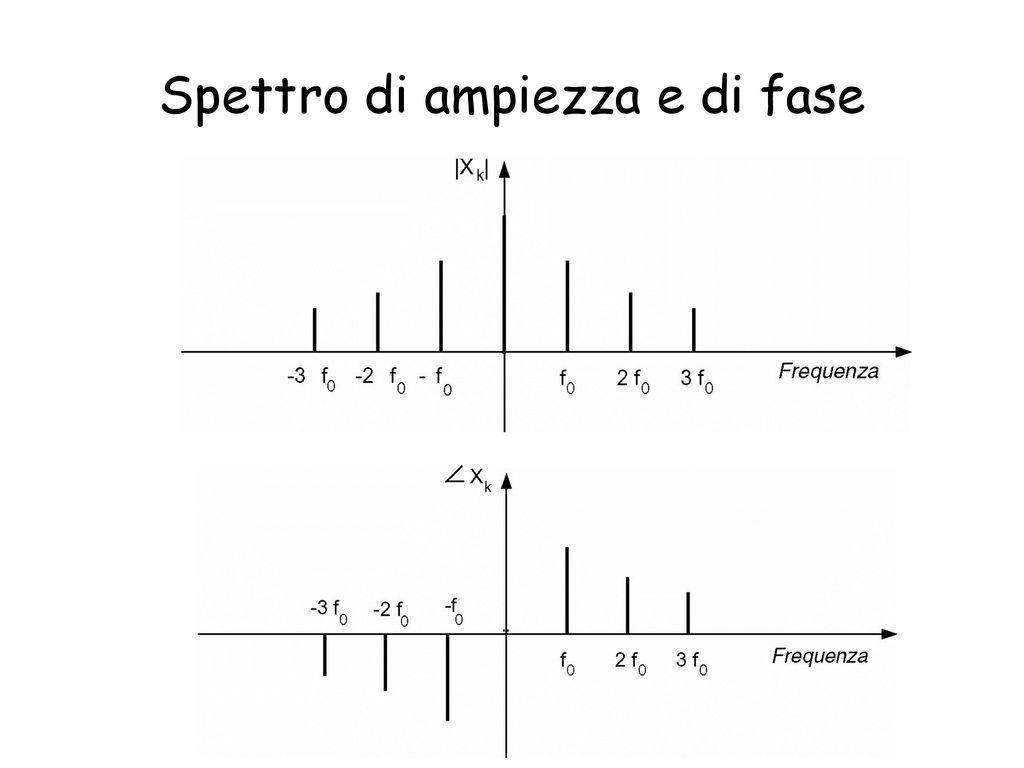
\includegraphics[width=1.0\textwidth]{images/spettro_di_ampiezza_e_di_fase.jpg}
	\caption{Spettro di ampiezza e di fase.}
\end{figure}

%-------------------------------------------------------------------------------
% Subsubsection: Simmetria pari per il modulo
%-------------------------------------------------------------------------------

\subsubsection{Simmetria pari per il modulo}
\begin{equation}
	\abs{X_n} = \abs{X_{-n}}
\end{equation}
Sia $f(x)$ una funzione a valori reali di variabile reale e sia $D \subset
\mathbb{R}$ il suo dominio. Allora $f$ \`e [aro se per ogni $x \in D$ vale
l'equazione:
\[
	f(x) = f(-x).
\]
Geometricamente, il grafico di una funzione pari \`e simmetrico rispetto
all'asse $y$.\\
\\
Il nome \textbf{pari} deriva dal fatto che le serie di Taylor di una funzione
pari centrata nell'origine contengono solo potenze pari.\\
\\
Esempi di funzioni pari sono $x^2$, $x^4$, $cos(x)$, $cosh(x)$.\\
\\
Esempio pratico:
\[
	y = x^2 - 1 \Longrightarrow f(-x) = (-x)^2 - 1 = x^2 - 1 = f(x).
\]

%-------------------------------------------------------------------------------
% Subsubsection: Simmetria dispari per la fase
%-------------------------------------------------------------------------------

\subsubsection{Simmetria dispari per la fase}
\begin{equation}
	\angle X_n = - \angle X_{-n}
\end{equation}
Sia $f(x)$ una funzione a valori reali di variabile reale e sia $D \subset
\mathbb{R}$ il suo dominio. Allora $f$ \`e dispari se per ogni $x \in D$
sussiste l'equazione:
\[
	f(-x) = - f(x),
\]
vale a dire
\[
	f(x) = - f(-x).
\]
Geometricamente, il grafico di una funzione dispari \`e simmetrico rispetto
all'origine degli assi.\\
\\
Il nome \textbf{dispari} deriva dal fatto che le serie di Taylor di una funzione
dispari centrate nell'origine contengono solo potenze dispari.\\
\\
Esempi di funzioni dispari sono $x$, $x^3•$, $sin(x)$, $sinh(x)$.\\
\\
Esempio pratico:
\[
	y = x^3 - x \Longrightarrow f(-x) = (-x)^3 - (-x) = -x^3 + x =
	-(x^3 - x) = -f(x).
\]

%-------------------------------------------------------------------------------
% Subsection: Trasformata di un segnale (periodico) reale e pari
%-------------------------------------------------------------------------------

\newpage
\subsection{Trasformata di un segnale (periodico) reale e pari}
Si consideri un segnale periodico
\[
	x(t) = x(t + T_0) \quad \forall t,
\]
reale
\[
	x(t) = x^*(t),
\]
e pari
\[
	x(t) = x(-t).
\]
In tal caso, il generico coefficiente di Fourier di $x(t)$ \`e una funzione pari
di $n$:
\[
	X_n = X_{-n}.
\]
\begin{proof}
\[
	X_{-n} = \frac{1}{T_0} \int\displaylimits_{-T_0/2}^{T_0/2} x(t)
	e^{-j 2 \pi (-n) f_0 t} \dt = \frac{1}{T_0}
	\int\displaylimits_{-T_0/2}^{T_0/2} x(t) e^{j 2 \pi n f_0 t} \dt =
\]
\[
	\footnote{Poniamo ora $t = -t^{'}$.}= \frac{1}{T_0}
	\int\displaylimits_{T_0/2}^{-T_0/2} x(-t^{'})
	e^{-j 2 \pi n f_0 t^{'}} -\dt^{'} = \frac{1}{T_0}
	\int\displaylimits_{-T_0/2}^{T_0/2} x(-t^{'}) e^{-j 2 \pi n f_0 t^{'}}
	\dt^{'} = 
\]
\[
	\footnote{Dato che $x(t) = x(-t)$.}= \frac{1}{T_0}
	\int\displaylimits_{-T_0/2}^{T_0/2} x(t^{'})
	e^{-j 2 \pi n f_0 t^{'}} \dt^{'} = X_n.
\]
\end{proof}
\noindent
Che dimostra la nostra tesi.
\bigbreak
Ora, dato che in generale sappiamo che $X_{-n} = X_n^*$, ne segue che $X_n$ \`e
sia pari che reale ed \`e quindi possibile riscrivere la Serie di Fourier per
$x(t)$ in forma semplificata. Infatti:
\[
	x(t) = \sum_{n = -\infty}^{+\infty} X_n e^{j 2 \pi n f_0 t} = X_0 +
	\sum_{n = 1}^{+\infty} X_n e^{j 2 \pi n f_0 t} + \sum_{n = -\infty}^{-1}
	X_n e^{j 2 \pi n f_0 t} =
\]
\[
	= X_0 + \sum_{n = 1}^{+\infty} X_n e^{j 2 \pi n f_0 t} +
	\sum_{n = 1}^{+\infty} X_{-n} e^{j 2 \pi (-n) f_0 t} =
\]
\[
	= X_0 + \sum_{n = 1}^{+\infty} X_n e^{j 2 \pi n f_0 t} +
	\sum_{n = 1}^{+\infty} X_{-n} e^{-j 2 \pi n f_0 t} =
\]
\[
	\footnote{$X_n = X_{-n}$. dato che $x(t)$ \`e un segnale pari.}= X_0 +
	\sum_{n = 1}^{+\infty} X_n e^{j 2 \pi n f_0 t} + \sum_{n = 1}^{+\infty}
	X_n e^{-j 2 \pi n f_0 t} =
\]
\[
	= X_0 + \sum_{n = 1}^{+\infty} X_n \left( e^{j 2 \pi n f_0 t} +
	e^{-j 2 \pi n f_0 t}\right) =
\]
\[
	= X_0 + 2 \cdot \sum_{n = 1}^{+\infty} X_n \left(
	\frac{e^{j 2 \pi n f_0 t} + e^{-j 2 \pi n f_0 t}}{2} \right) =
\]
\[
	= X_0 + 2 \cdot \sum_{n = 1}^{+\infty} X_n \cos(2 \pi n f_0 t).
\]
Abbiamo quindi semplificato l'espressione in serie di Fourier eliminando i
termini sinusoidale per i segnali periodici pari.\\ Questo risultato \`e
logicamente giustificabile se si riflette sul fatto che il coseno \`e una
funzione pari mentre il seno \`e una funzione dispari e quindi poco si presta a
rappresentare l'andamento periodico di un segnale pari.

%-------------------------------------------------------------------------------
% Subsection: Trasformata di un segnale (periodico) reale e dispari
%-------------------------------------------------------------------------------

\newpage
\subsection{Trasformata di un segnale (periodico) reale e dispari}
Si consideri un segnale periodico
\[
	x(t) = x(t + T_0) \quad \forall t,
\]
reale
\[
	x(t) = x^*(t),
\]
e dispari
\[
	x(t) = -x(-t).
\]
In tal caso, il generico coefficiente di Fourier di $x(t)$ \`e una funzione
dispari di $n$:
\[
	X_n = -X_{-n}.
\]
\begin{proof}
\[
	-X_{-n} = -\frac{1}{T_0} \int\displaylimits_{-T_0/2}^{T_0/2} x(t)
	e^{-j 2 \pi (-n) f_0 t} \dt = \frac{1}{T_0}
	\int\displaylimits_{-T_0/2}^{T_0/2} -x(t) e^{j 2 \pi n f_0 t} \dt =
\]
\[
	\footnote{Poniamo ora $t = -t^{'}$.}= \frac{1}{T_0}
	\int\displaylimits_{T_0/2}^{-T_0/2} -x(-t^{'}) e^{-j 2 \pi n f_0 t^{'}}
	-\dt^{'} = \frac{1}{T_0} \int\displaylimits_{-T_0/2}^{T_0/2} -x(-t^{'})
	e^{-j 2 \pi n f_0 t^{'}} \dt^{'} = 
\]
\[
	\footnote{Dato che $x(t) = -x(-t)$.}= \frac{1}{T_0}
	\int\displaylimits_{-T_0/2}^{T_0/2} x(t^{'}) e^{-j 2 \pi n f_0 t^{'}}
	\dt^{'} = X_n.
\]
\end{proof}
\noindent
Che dimostra la nostra tesi.
\bigbreak
Ora, dato che in generale sappiamo che $X_{-n} = X_n^*$, ne segue che $X_n$ \`e
sia dispari che reale ed \`e quindi possibile riscrivere la Serie di Fourier per
$x(t)$ in forma semplificata. Infatti:
\[
	x(t) = \sum_{n = -\infty}^{+\infty} X_n e^{j 2 \pi n f_0 t} = X_0 +
	\sum_{n = 1}^{+\infty} X_n e^{j 2 \pi n f_0 t} + \sum_{n = -\infty}^{-1}
	X_n e^{j 2 \pi n f_0 t} =
\]
\[
	= X_0 + \sum_{n = 1}^{+\infty} X_n e^{j 2 \pi n f_0 t} +
	\sum_{n = 1}^{+\infty} X_{-n} e^{j 2 \pi (-n) f_0 t} =
\]
\[
	= X_0 + \sum_{n = 1}^{+\infty} X_n e^{j 2 \pi n f_0 t} +
	\sum_{n = 1}^{+\infty} X_{-n} e^{-j 2 \pi n f_0 t} =
\]
\[
	\footnote{$X_n = -X_{-n}$. dato che $x(t)$ \`e un segnale dispari.}= X_0
	+ \sum_{n = 1}^{+\infty} X_n e^{j 2 \pi n f_0 t} +
	\sum_{n = 1}^{+\infty} (-X_n) e^{-j 2 \pi n f_0 t} =
\]
\[
	= X_0 + \sum_{n = 1}^{+\infty} X_n e^{j 2 \pi n f_0 t} -
	\sum_{n = 1}^{+\infty} X_n e^{-j 2 \pi n f_0 t} =
\]
\[
	= X_0 + \sum_{n = 1}^{+\infty} X_n \left( e^{j 2 \pi n f_0 t} -
	e^{-j 2 \pi n f_0 t}\right) =
\]
\[
	= X_0 + 2 j \cdot \sum_{n = 1}^{+\infty} X_n \left(
	\frac{e^{j 2 \pi n f_0 t} - e^{-j 2 \pi n f_0 t}}{2 j} \right) =
\]
\[
	= X_0 + 2 j \cdot \sum_{n = 1}^{+\infty} X_n \sin(2 \pi n f_0 t).
\]
Abbiamo quindi semplificato l'espressione in serie di Fourier eliminando i
termini cosinusoidale per i segnali periodici dispari.\\ Questo risultato \`e
logicamente giustificabile se si riflette sul fatto che il seno \`e una funzione
dispari mentre il coseno \`e una funzione pari e quindi poco si presta a
rappresentare l'andamento periodico di un segnale dispari.

%-------------------------------------------------------------------------------
% Subsection: Trasformata di un segnale (periodico) reale alternativo
%-------------------------------------------------------------------------------

\newpage
\subsection{Trasformata di un segnale (periodico) reale alternativo}
Si consideri un segnale periodico
\[
	x(t) = x(t + T_0) \quad \forall t,
\]
reale
\[
	x(t) = x^*(t),
\]
e alternativo
\[
	x(t) = -x\left(t + \frac{T_0}{2}\right).
	\footnote{L'andamento del segnale in un qualunque semiperiodo
	$t_0 \leq t < t_0 + T_0/2$ \`e identico all'andamento nel semiperiodo
	precedente $t_0 - T_0/2 \leq t < t$, cambiato di segno.}
\]
\begin{figure}[H]
	\centering
	\captionsetup{justification=centering}
	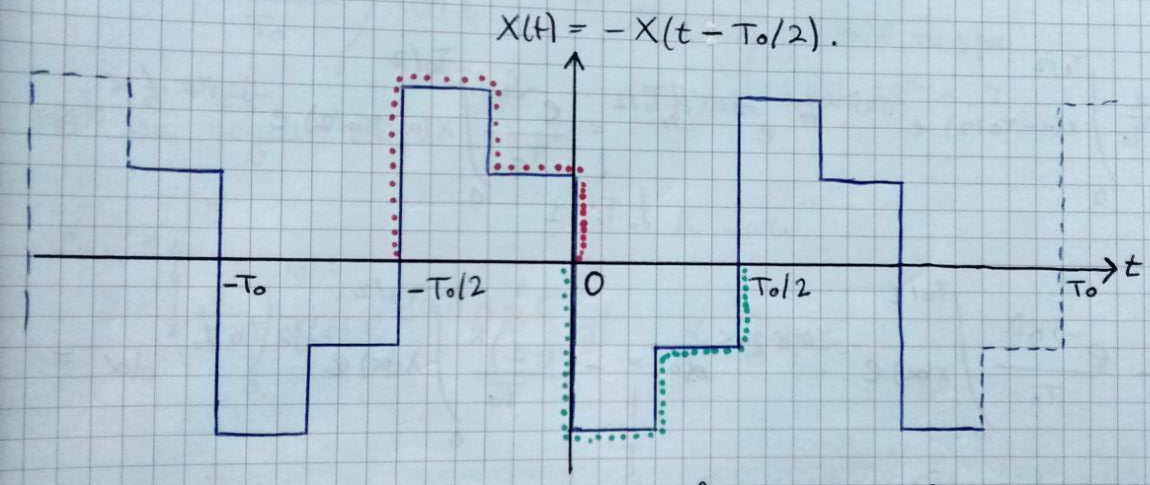
\includegraphics[width=1.0\textwidth]{images/segnale_alternativo.jpg}
	\caption{Rappresentazione grafica di un segnale alternativo.}
\end{figure}
In tal caso, il generico coefficiente $X_n$ di Fourier di $x(t)$ \`e
\textit{nullo} per tutti i valori pari dell'indice $n$:
\begin{equation}
	X_n =
	\begin{cases}
		\frac{2}{T_0} \int\displaylimits_{0}^{T_0/2} x(t)
		e^{-j 2 \pi n f_0 t} \dt \quad\quad\quad\quad n \ dispari\\
		0 \quad\quad\quad\quad\quad\quad\quad\quad\quad\quad\quad\quad
		\quad \ \ \ n \ pari
	\end{cases}.
\end{equation}
\begin{proof}
\[
	X_{n} = \frac{1}{T_0} \int\displaylimits_{-T_0/2}^{T_0/2} x(t)
	e^{-j 2 \pi n f_0 t} \dt =
\]
\[
	\footnote{Avendo suddiviso l'intervallo di integrazione
	$[-T_0/2, T_0/2]$ in due smeiperiodi.}= \frac{1}{T_0}
	\int\displaylimits_{-T_0/2}^{0} x(t) e^{-j 2 \pi n f_0 t} \dt +
	\frac{1}{T_0} \int\displaylimits_{0}^{T_0/2} x(t) e^{-j 2 \pi n f_0 t}
	\dt =
\]
Il primo integrale pu\`o essere riscritto come
\[
	\footnote{Poniamo $t^{'} = t + \frac{T_0}{2}$ nel primo integrale.
	Quindi $t = t^{'} - \frac{T_0}{2}$, e se $t$ va da $-\frac{T_0}{2}$ a
	$0$, allora $t^{'} = t + \frac{T_0}{2}$ va da $0$ a $\frac{T_0}{2}$.}=
	\frac{1}{T_0} \int\displaylimits_{0}^{T_0/2} x\left(t^{'} -
	\frac{T_0}{2}\right) e^{-j 2 \pi n f_0 \left(t^{'} -
	\frac{T_0}{2}\right)} \dt^{'} = \frac{1}{T_0}
	\int\displaylimits_{0}^{T_0/2} -x(t^{'}) e^{-j 2 \pi n f_0 \left(t^{'} -
	\frac{T_0}{2}\right)} \dt^{'} =
\]
\[
	= \frac{1}{T_0} \int\displaylimits_{0}^{T_0/2} -x(t^{'})
	e^{-j 2 \pi n f_0 t^{'}} e^{j 2 \pi n f_0 \frac{T_0}{2}} \dt^{'} =
	\frac{1}{T_0} \int\displaylimits_{0}^{T_0/2} -x(t^{'})
	e^{-j 2 \pi n f_0 t^{'}} e^{j \pi n} \dt^{'} =
\]
\[
	\footnote{$e^{j \pi n} = \cos(\pi n) - j \sin(\pi n) = \pm 1$.}=
	\frac{1}{T_0} \int\displaylimits_{0}^{T_0/2} -x(t^{'})
	e^{-j 2 \pi n f_0 t^{'}} (-1)^{n} \dt^{'} = (-1)^{n} \cdot
	\frac{1}{T_0} \int\displaylimits_{0}^{T_0/2} -x(t^{'})
	e^{-j 2 \pi n f_0 t^{'}} \dt^{'} =
\]
\[
	= -\frac{(-1)^{n}}{T_0} \int\displaylimits_{0}^{T_0/2} x(t)
	e^{-j 2 \pi n f_0 t} \dt.
\]
Ora, sostituendo questo risultato nell'integrale iniziale
\[
	= -\frac{(-1)^{n}}{T_0} \int\displaylimits_{0}^{T_0/2} x(t)
	e^{-j 2 \pi n f_0 t} \dt + \frac{1}{T_0} \int\displaylimits_{0}^{T_0/2}
	x(t^{'}) e^{-j 2 \pi n f_0 t^{'}} \dt^{'} =
\]
\[
	= \left[1 - (-1)^{n}\right] \cdot \frac{1}{T_0}
	\int\displaylimits_{0}^{T_0/2} x(t^{'}) e^{-j 2 \pi n f_0 t^{'}}
	\dt^{'}.
\]
Ne segue quindi che
\[
	X_n = \frac{2}{T_0} \int\displaylimits_{0}^{T_0/2} x(t)
	e^{-j 2 \pi n f_0 t} \dt \quad\quad\quad n \ dispari
\]
\[
	X_n = 0 \quad\quad\quad\quad\quad\quad\quad\quad\quad\quad\quad\quad
	\quad n \ pari.
\]
\end{proof}
\noindent
Che dimostra la nostra tesi.

%-------------------------------------------------------------------------------
% Subsection: Simmetrie della Trasformata Continua di Fourier (TCF)
%-------------------------------------------------------------------------------

\newpage
\subsection{Simmetrie della Trasformata Continua di Fourier (TCF)}
La funzione complessa $X(f)$ pu\`o essere rappresentata in forma polare o in
forma rettangolare:
\begin{equation}
	X(f) = R(f) + j I(f)
\end{equation}
dove $R(f)$ e $I(f)$ ne rappresentano rispettivamente la parte reale e la parte
immaginaria.\\
Vogliamo ora stabilire in che modo le propriet\`a della funzione $x(t)$ si
riflettano sulla sua trasformata.

%-------------------------------------------------------------------------------
% Subsubsection: Simmetrie della TCF: Simmetria Hermitiana
%-------------------------------------------------------------------------------

\subsubsection{Simmetrie della TCF: Simmetria Hermitiana}
Supponiamo che $x(t)$ sia una funzione \textit{reale}:
\[
	x(t) = x^*(t)
\]
in tal caso $X(f)$ \`e \textit{Hermitiana}
\[
	X(-f) = X^*(f).
\]
In tal caso le funzione $R(f)$ e $I(f)$ si ricavano immediatamente dalle
seguenti relazioni
\[
	R(f) = \int\displaylimits_{-\infty}^{+\infty} x(t) \cos(2 \pi f t) \dt,
\]
\[
	I(f) = -\int\displaylimits_{-\infty}^{+\infty} x(t) \sin(2 \pi f t) \dt.
\]
Da queste espressioni si vede chiaramente che
\[
	R(f) = R(-f),
\]
\[
	I(f) = -I(f),
\]
ovvero la parte reale della trasformata di un segnale reale \`e una funzione
\textit{pari} della frequenza, mentre la parte immaginaria ne \`e una funzione
\textit{dispari}.\\
La medesima propriet\`a si riflette ovviamente anche nelle funzioni $A(f)$ e
$\vartheta(f)$:
\[
	A(f) = A(-f),
\]
\[
	\vartheta(f) = - \vartheta(-f),
\]
per cui lo spettro di ampiezza di un segnale reale \`e una funzione pari, mentre
il suo spettro di fase \`e dispari.
\begin{proof}
\[
	X(-f) = \int\displaylimits_{-\infty}^{+\infty} x(t) \cdot
	e^{-j 2 \pi (-f) t} \dt = \int\displaylimits_{-\infty}^{+\infty} x(t)
	\cdot e^{j 2 \pi f t} \dt =
\]
\[
	= \int\displaylimits_{-\infty}^{+\infty} x^*(t) \cdot e^{j 2 \pi f t}
	\dt = \int\displaylimits_{-\infty}^{+\infty} \left[x(t) \cdot
	e^{-j 2 \pi f t}\right]^* \dt =
\]
\[
	= \left[\int\displaylimits_{-\infty}^{+\infty} x(t) \cdot
	e^{-j 2 \pi f t} \dt\right]^* = X^*(f).
\]
\end{proof}

%-------------------------------------------------------------------------------
% Subsubsection: Simmetrie della TCF: Segnali reali e pari
%-------------------------------------------------------------------------------

\newpage
\subsubsection{Simmetrie della TCF: Segnali reali e pari}
Supponiamo adesso che $x(t)$ sia un segnale \textit{reale e pari}
\[
	x(t) = x^*(t) \quad\quad , \quad\quad x(t) = x(-t).
\]
Le relazioni che esprimono la parte reale e quella immaginaria del suo
coefficiente di Fourier si semplificano rispettivamente in
\[
	R(f) = 2 \int\displaylimits_{0}^{\infty} x(t) \cos(2 \pi f t) \dt,
\]
\[
	I(f) = 0.
\]
Ovvero, la trasformata di un segnale reale e pari \`e una funzione
\textit{reale e pari} della frequenza
\[
	X(f) = X^*(f) \quad\quad , \quad\quad X(f) = X(-f).
\]
\begin{proof}
$X(f) = X^*(f)$
\[
	X(f) = \int\displaylimits_{-\infty}^{+\infty} x(t) \cdot
	e^{-j 2 \pi f t} \dt =\footnote{Poniamo $t = -t^{'}$, $dt = dt^{'}$, se
	$t$ va da $-\infty$ a $+\infty$, allora $t^{'}$ va da $+\infty$ a
	$-\infty$.} \int\displaylimits_{+\infty}^{-\infty} x(-t^{'}) \cdot
	e^{-j 2 \pi f (-t^{'})} \ -dt^{'} =
\]
\[
	= - \int\displaylimits_{+\infty}^{-\infty} x(-t^{'}) \cdot
	e^{j 2 \pi f t^{'}} \ dt^{'} = \int\displaylimits_{-\infty}^{+\infty}
	x(-t^{'}) \cdot e^{j 2 \pi f t^{'}} \ dt^{'} =
\]
\[
	= \int\displaylimits_{-\infty}^{+\infty} x(t^{'}) \cdot
	e^{j 2 \pi f t^{'}} \ dt^{'} = \int\displaylimits_{-\infty}^{+\infty}
	x^*(t^{'}) \cdot e^{j 2 \pi f t^{'}} \ dt^{'} =
\]
\[
	= \int\displaylimits_{-\infty}^{+\infty} \left[x(t^{'}) \cdot
	e^{-j 2 \pi f t^{'}}\right]^* \ dt^{'} = \left[
		\int\displaylimits_{-\infty}^{+\infty} x(t^{'}) \cdot
		e^{-j 2 \pi f t^{'}} \ dt^{'}\right]^* = X^*(f).
\]
\end{proof}
\begin{proof}
$X(f) = X(-f)$
\[
	X(f) = \int\displaylimits_{-\infty}^{+\infty} x(t) \cdot 
	e^{-j 2 \pi f t} \dt = \int\displaylimits_{+\infty}^{-\infty} x(-t^{'}) 
	\cdot e^{-j 2 \pi f (-t^{'})} \ -dt^{'} =
\]
\[
	= - \int\displaylimits_{+\infty}^{-\infty} x(-t^{'}) \cdot 
	e^{-j 2 \pi (-f) t^{'}} \ dt^{'} = 
	\int\displaylimits_{-\infty}^{+\infty} x(t^{'}) \cdot 
	e^{-j 2 \pi (-f) t^{'}} \ dt^{'} = X(-f).
\]
\end{proof}

%-------------------------------------------------------------------------------
% Subsubsection: Simmetrie della TCF: Segnali reali e dispari
%-------------------------------------------------------------------------------

\newpage
\subsubsection{Simmetrie della TCF: Segnali reali e dispari}
Supponiamo adesso che $x(t)$ sia un segnale \textit{reale e dispari}
\[
	x(t) = x^*(t) \quad\quad , \quad\quad x(t) = -x(-t).
\]
Le relazioni che esprimono al parte reale e quella immaginaria del suo
coefficiente di Fourier si semplificano rispettivamente in
\[
	R(f) = 0,
\]
\[
	I(f) = -2 \int\displaylimits_{0}^{\infty} x(t) sin(2 \pi f t) \dt.
\]
Ovvero, la trasformata di un segnale reale e dispari \`e una funzione
\textit{immaginaria pura e dispari} della frequenza
\[
	X(f) = -X(-f) \quad\quad , \quad\quad X(f) \ immaginario \ puro.
\]
\begin{proof}
$X(f) = -X(-f)$
\[
	-X(-f) = -\int\displaylimits_{-\infty}^{+\infty} x(t) \cdot
	e^{-j 2 \pi (-f) t} \dt = \int\displaylimits_{-\infty}^{+\infty} -x(t)
	\cdot e^{j 2 \pi f t} \dt =
\]
\[
	= \int\displaylimits_{-\infty}^{+\infty} -x(-t^{'}) \cdot
	e^{j 2 \pi f (-t^{'})} \dt = \int\displaylimits_{-\infty}^{+\infty}
	x(t^{'}) \cdot e^{-j 2 \pi f t^{'}} \dt = X(f).
\]
\end{proof}

%-------------------------------------------------------------------------------
% Subsection: Teoremi sulla trasformata continua di Fourier
%-------------------------------------------------------------------------------

\newpage
\subsection{Teoremi sulla trasformata continua di Fourier}
Dalla definizione di trasformata, seguono facilmente alcune ulteriori
propriet\`a, che chiameremo \textit{teoremi}, estremamente utili nel calcolo
delle trasformate dei segnali e comunque nell'uso dell'analisi di Fourier di
carattere applicativo.

%-------------------------------------------------------------------------------
% Subsubsection: Linearita' della TCF
%-------------------------------------------------------------------------------

\subsubsection{Linearit\`a della TCF}
Pu\`o essere conveniente in molti casi esprimere un segnale $x(t)$ come
combinazione lineare di due segnali $x_1(t)$ e $x_2(t)$:
\[
	x(t) = a \cdot x_1(t) + b \cdot x_2(t),
\]
con $a$ e $b$ costanti. Indicando come di consueto con $X_1(f)$ e $X_2(f)$ le
trasformate rispettivamente dei segnali $x_1(t)$ e $x_2(t)$, la trasformata
$X(f)$ di $x(t)$ \`e allora
\[
	X(f) = a \cdot X_1(f) + b \cdot X_2(f).
\]
\begin{proof}
Infatti, applicando semplicemente la definizione trasformata, la tesi segue
sfruttando la propriet\`a di linearit\`a dell'integrale stesso
\[
	X(f) = \int\displaylimits_{-\infty}^{+\infty} x(t) \cdot
	e^{-j 2 \pi f t} \dt = \int\displaylimits_{-\infty}^{+\infty} [a 
	\cdot x_1(t) + b \cdot x_2(t)] \cdot e^{-j 2 \pi f t} \dt =
\]
\[
	= \int\displaylimits_{-\infty}^{+\infty} a \cdot x_1(t) \cdot 
	e^{-j 2 \pi f t} \dt + \int\displaylimits_{-\infty}^{+\infty} b 
	\cdot x_2(t) \cdot e^{-j 2 \pi f t} \dt =
\]
\[
	= a \cdot \int\displaylimits_{-\infty}^{+\infty} x_1(t) \cdot 
	e^{-j 2 \pi f t} \dt + b \cdot \int\displaylimits_{-\infty}^{+\infty} 
	x_2(t) \cdot e^{-j 2 \pi f t} \dt =
\]
\[
	= a \cdot X_1(f) + b \cdot X_2(f).
\]
\end{proof}

%-------------------------------------------------------------------------------
% Subsubsection: Dualita' della TCF
%-------------------------------------------------------------------------------

\newpage
\subsubsection{Dualit\`a della TCF}
La similitudine tra le relazioni di trasformata e antitrasformata intese come
"operatori" sulle funzioni rispettivamente $x(t)$ e $X(f)$ permette di risolvere
una questione: se $X(f)$ indica la trasformata del segnale $x(t)$, qual \`e la
trasformata del segnale \textit{temporale} $X(t)$, avente cio\`e lo stesso
andamento temporale originariamente posseduto nell'ambito frequenziale dalla
trasformata di $x(t)$? La risposta \`e la seguente: se
\[
	x(t) \iff X(f)
\]
allora
\[
	X(t) \iff x(-f).
\]
Infatti, sappiamo che il segnale $x(t)$ \`e legato alla sua trasformata dalla
relazione
\[
	x(t) = \int\displaylimits_{-\infty}^{+\infty} X(f) e^{j 2 \pi f t} \ df.
\]
Scambiando formalmente le variabili $t$ ed $f$ nella precedente relazione, si
ricava
\[
	x(f) = \int\displaylimits_{-\infty}^{+\infty} X(t) e^{j 2 \pi t f} \ dt.
\]
Se poi in questa relazione si effettua un cambiamento di variabile sostituendo
alla variabile $f$ la variabile $-f$, si ottiene
\[
	x(-f) = \int\displaylimits_{-\infty}^{+\infty} X(t) e^{-j 2 \pi f t} \dt
\]
che dimostra la tesi iniziale.

%-------------------------------------------------------------------------------
% Subsubsection: Teorema del ritardo
%-------------------------------------------------------------------------------

\newpage
\subsubsection{Teorema del ritardo}
Come viene modificata la trasformata di un segnale se questo viene traslato
sull'asse dei tempi (cio\`e, anticipato o ritardato)? Sia dunque $X(f)$ la
trasformata del segnale $x(t)$; allora la trasformata del segnale traslato a
destra della quantit\`a $t_0$
\[
	y(t) = x(t - t_0)
\]
\`e
\[
	Y(f) = X(f) e^{-j 2 \pi f t_0}.
\]
Questa operazione corrisponde evidentemente a un ritardo se $t_0 > 0$ e ad un
anticipo se $t_0 < 0$.
\begin{proof}
Applicando la definizione di trasformata si ha
\[
	Y(f) = \int\displaylimits_{-\infty}^{+\infty} y(t) e^{-j 2 \pi f t} \dt
	= \int\displaylimits_{-\infty}^{+\infty} x(t - t_0) e^{-j 2 \pi f t} \dt
	=
\]
\[
	\footnote{Poniamo $t' = t - t_0$.}=
	\int\displaylimits_{-\infty}^{+\infty} x(t') e^{-j 2 \pi f (t' + t_0)}
	\dt ' =	\int\displaylimits_{-\infty}^{+\infty} x(t') e^{-j 2 \pi f t'}
	e^{-j 2 \pi f t_0} \dt ' =
\]
\[
	= \int\displaylimits_{-\infty}^{+\infty} x(t') e^{-j 2 \pi f t'} \dt '
	\cdot e^{-j 2 \pi f t_0}
	= X(f) e^{-j 2 \pi f t_0}.
\]
\end{proof}
Questa propriet\`a mostra che un ritardo temporale modifica lo spettro di fase
della trasformata del segnale ma \textit{non cambia il suo spettro di ampiezza}.
Infatti, il teorema del ritardo si traduce nelle relazioni
\[
	\abs{Y(f)} = \abs{X(f)},
\]
\[
	\angle Y(f) = \angle X(f) - 2 \pi f t_0.
\]

%-------------------------------------------------------------------------------
% Subsubsection: Teorema del cambiamento di scala
%-------------------------------------------------------------------------------

\newpage
\subsubsection{Teorema del cambiamento di scala}
Si consideri la situazione generale in cui due segnali siano legati dalla
relazione
\[
	y(t) = x(\alpha t).
\]
Cio\`e si effettua un cambiamento della scala temporale. Moltiplicando la
variabile indipendente $t$ del segnale $x(t)$ per coefficiente $\alpha$ si
producono i seguenti effetti:
\begin{itemize}
	\item $\abs{\alpha} > 1$ $\rightarrow$ \textit{compressione} della scala
		dei tempi
	\item $\abs{\alpha} < 1$ $\rightarrow$ \textit{dilatazione} della scala
		dei tempi
	\item $\alpha < 0$ \ \ $\rightarrow$ \textit{inversione} della scala dei
		tempi
\end{itemize}
In altri termini, se $\abs{\alpha} < 1$ l'evoluzione del segnale viene
"rallentata", viceversa se $\abs{\alpha} > 1$ il segnale viene "accelerato".
Operazoini di questo tipo vengono effettuate correntemente nell'elaborazione dei
segnali registrando il segnale ad una certa velocit\`a e riproducendolo a
velocit\`a diversa.
\bigbreak\noindent
Allora
\[
	Y(f) = \frac{1}{\abs{\alpha}} \cdot X\left(\frac{f}{\alpha}\right)
\]
\begin{proof}
$\alpha > 0$
\[
	Y(f) = \int\displaylimits_{-\infty}^{+\infty} y(t) e^{-j 2 \pi f t} \dt
	= \int\displaylimits_{-\infty}^{+\infty} x(\alpha t) e^{-j 2 \pi f t}
	\dt =
\]
\[
	\footnote{Poniamo $t' = \alpha t$, da cui $dt' = d(\alpha t)$ e $dt' =
	\alpha dt \rightarrow dt = dt'/\alpha$.}= \int\displaylimits_{-\infty}
	^{+\infty} x(t') e^{-j 2 \pi f \frac{t'}{\alpha}} \frac{\dt'}{\alpha} =
	\frac{1}{\alpha} \int\displaylimits_{-\infty}^{+\infty} x(t')
	e^{-j 2 \pi \frac{f}{\alpha}t'} \dt' =
\]
\[
	= \frac{1}{\alpha} X\left(\frac{f}{\alpha}\right) \quad , \quad
	\alpha > 0.
\]
\end{proof}
\begin{proof}
$\alpha < 0$
\[
	Y(f) = \int\displaylimits_{-\infty}^{+\infty} y(t) e^{-j 2 \pi f t} \dt
	= \int\displaylimits_{-\infty}^{+\infty} x(\alpha t) e^{-j 2 \pi f t}
	\dt =
\]
\[
	\footnote{Poniamo $t' = \alpha t$, da cui $t = \frac{t'}{\alpha}$,
	$dt' = d(\alpha t) \rightarrow dt' = \alpha \cdot dt'$,
	$dt = \frac{dt'}{\alpha}$.}=
	\int\displaylimits_{-\infty}^{+\infty} x(t')
	e^{-j 2 \pi f \frac{t'}{\alpha}} -\frac{\dt}{\alpha} = -\frac{1}{\alpha}
	\int\displaylimits_{-\infty}^{+\infty} x(t')
	e^{-j 2 \pi \frac{f}{\alpha} t'} \dt' =
\]
\[
	= -\frac{1}{\alpha} X\left(\frac{f}{\alpha}\right) \quad , \quad
	\alpha < 0.
\]
\end{proof}
I risultati ottenuti per $\alpha > 0$ e $\alpha < 0$ possono allora essere
riassunti con
\[
	x(\alpha t) \iff \frac{1}{\abs{\alpha}} X\left(\frac{f}{\alpha}\right).
\]
Si nota quindi che una dilatazione dell'asse dei tempi comporta una compressione
dell'asse delle frequenze, e viceversa. Se infatti il segnale viene
"rallentato", vengono a predominare le componenti frequenziali a bassa
frequenza, che sono responsabili per cos\`i dire dell'evoluzione del segnale; lo
spettro allora di "addensa" nell'intorno della frequenza nulla.

%-------------------------------------------------------------------------------
% Subsection: Teorema della Modulazione
%-------------------------------------------------------------------------------

\newpage
\subsection{Teorema della Modulazione}
In telecomunicazioni ed elettronica con il termine modulazione si indica
l'insieme delle tecniche di trasmissione finalizzate ad imprimere un segnale
elettrico o elettromagnetico, detto modulante, generalmente contenente
informazione cio\`e variabile in maniera aleatoria nel tempo, su di un altro
segnale elettrico o elettromagnetico, detto portante, sviluppato ad alta
frequenza (frequenza portante $>>$ frequenza modulante). Il risultato della
modulazione \`e la conversione del segnale modulante dalla banda base alla
cosiddetta banda traslata (segnale modulato), secondo il teorema della
modulazione.
\begin{figure}[H]
	\centering
	\captionsetup{justification=centering}
	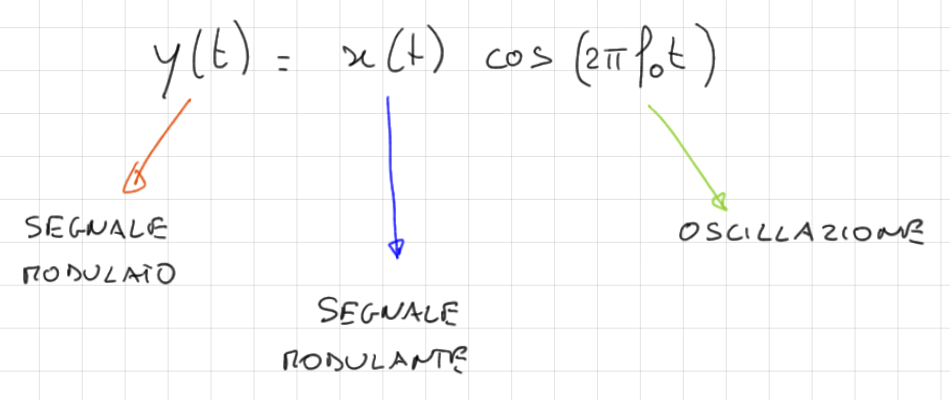
\includegraphics[width=1.0\textwidth]{images/modulato_modulante_oscillazione.png}
	\caption{Segnale modulato.}
\end{figure}
L'operazione inversa di ripristino del segnale informativo originario in banda
base \`e detto demodulazione. Il dispositivo in trasmissione che attua
l'operazione di modulazione sul segnale informativo \`e detto modulatore, mentre
il dispositivo in ricezione che attua l'operazione di demodulazione \`e detto
demodulatore, compresi rispettivamente nel trasmettitore e nel ricevitore. In
un sistema di ricetrasmissione tali sistemi vengono riuniti entrambi sotto la
dizione \textit{Modem} (dalla composizione di Modulazione e Demodulazione).\\
I segnali modulati possono rappresentare le informazioni pi\`u diverse: audio,
video, dati, ecc... L'onda portante \`e un'onda elettromagnetica o un segnale
elettrico a frequenza ben determinata (molto maggiore della frequenza del
segnale modulante), che pu\`o essere trasmessa in aria o nel vuoto (ad esempio
nelle radiocomunicazioni), o tramite altro mezzo fisico (ad esempio un cavo).
In caso di comunicazioni in fribra ottica la portante \`e la radiazione laser la
cui frequenza \`e tipicamente espressa come lunghezza d'onda.
\bigbreak
In generale, il motivo per cui si utilizzano le tecniche di modulazione risiede
nel fatto che i segnali rappresentanti le informazioni da trasmettere sono in
prevalenza di natura passa-basso (il loro contenuto spettrale \`e concentrato
per lo pi\`u a basse frequenze), mentre i canali trasmissivi che pi\`u
comunamente si utilizzano, per poter trasmettere segnali modulati
contemporaneamente, (come canali hertziani e fibre ottiche) sono tipicamente di
natura passa-banda cio\`e trasmettono in una banda a frequenza diversa da quella
del segnale informativo originario. In sostanza occorre quindi convertire in
frequenza, mediante tale tecnica, lo spettro del segnale rappresentante
l'informazione.
\begin{figure}[H]
	\centering
	\captionsetup{justification=centering}
	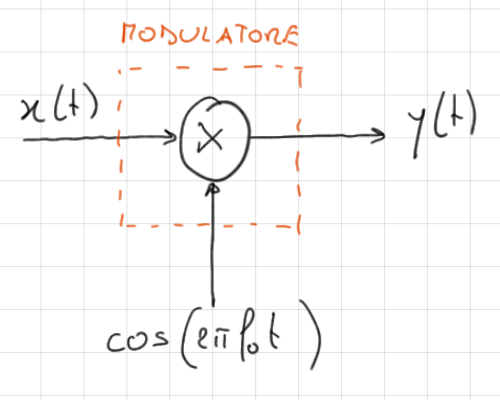
\includegraphics[width=0.5\textwidth]{images/modulatore.png}
	\caption{Modulatore.}
\end{figure}
Esistono diversi tipi di modulazione analogica, utilizzate nelle rispettive
trasmissioni analogiche:
\begin{itemize}
	\item AM - (Amplitude Modulation) modulazione di ampiezza;
	\item FM - (Frequency Modulation) modulazione di frequenza;
	\item PM - (Phase Modulation) modulazione di fase.
\end{itemize}
In sostanza, l'informazione da trasmettere pu\`o essere codificata all'interno
di variazioni di ampiezza, frequenza e fase, ed in ricezione dovr\`a essere
recuperata, ovvero demodulata dal segnale portante ricevuto.
\begin{figure}[H]
	\centering
	\captionsetup{justification=centering}
	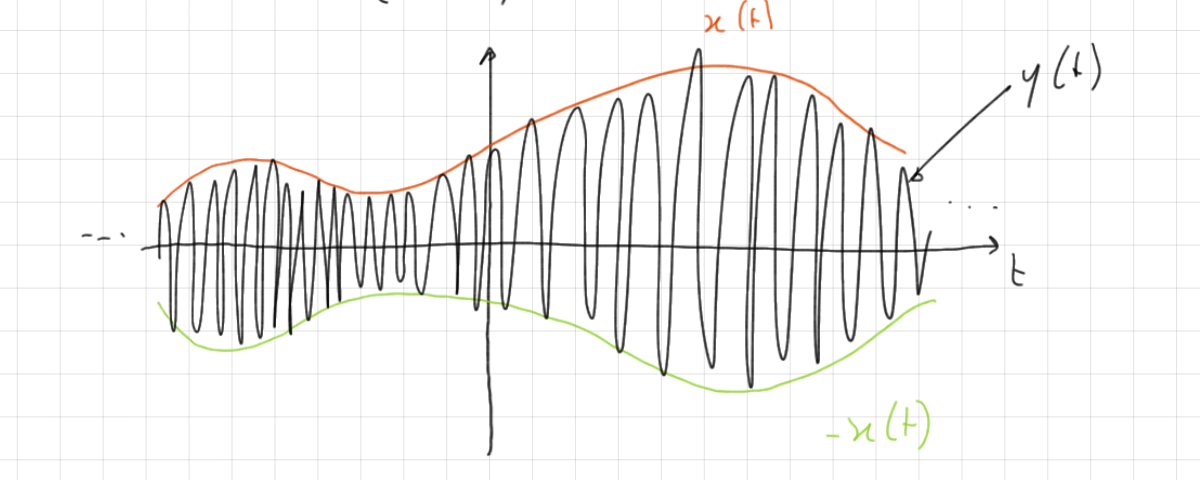
\includegraphics[width=1.0\textwidth]{images/segnale_modulato.png}
	\caption{Codifica dell'informazione da trasmettere.}
\end{figure}
Enunciamo ora formalmente il cosiddetto teorema della modulazione.

%-------------------------------------------------------------------------------
% Subsubsection: Modulazione con coseno
%-------------------------------------------------------------------------------

\newpage
\subsubsection{Modulazione con coseno}
Se, come di consueto, $x(t) \iff X(f)$, allora definendo
\[
	y(t) = x(t) \cdot \cos(2 \pi f_0 t)
\]
segue che
\[
	Y(f) = \frac{1}{2} \cdot X(f - f_0) + \frac{1}{2} X(f + f_0) =
	\frac{X(f - f_0) + X(f + f_0)}{2}.
\]
\begin{proof}
\[
	Y(f) = \int\displaylimits_{-\infty}^{+\infty} y(t) e^{-j 2 \pi f t} \dt
	= \int\displaylimits_{-\infty}^{+\infty} x(t) cos(2 \pi f_0 t)
	e^{-j 2 \pi f t} \dt =
\]
\[
	\footnote{$\cos(2 \pi f_0 t) = \frac{e^{j 2 \pi f_0 t} +
	e^{-j 2 \pi f_0 t}}{2}$} = \int\displaylimits_{-\infty}^{+\infty}
	x(t) \cdot \frac{e^{j 2 \pi f_0 t} + e^{-j 2 \pi f_0 t}}{2} \cdot
	e^{-j 2 \pi f t} \dt =
\]
\[
	= \int\displaylimits_{-\infty}^{+\infty} x(t) \cdot
	\frac{e^{-j 2 \pi (f - f_0) t} + e^{-j 2 \pi (f + f_0) t}}{2} \dt =
\]
\[
	= \frac{1}{2} \int\displaylimits_{-\infty}^{+\infty} x(t)
	e^{-j 2 \pi (f - f_0)t} \dt + \frac{1}{2}
	\int\displaylimits_{-\infty}^{+\infty} x(t) e^{-j 2 \pi (f + f_0) t} \dt
	=
\]
\[
	\frac{1}{2} X(f - f_0) + \frac{1}{2} X(f + f_0),
\]
che dimostra la tesi iniziale.
\end{proof}
Una prima conclusione che possiamo trarre \`e la seguente: se un segnale viene
moltiplicato per il fattore esponenziale complesso $e^{j 2 \pi f_0 t}$, la sua
trasformata di Fourier viene traslata attorno alla frequenza $f_0$. Questo
risultato rappresenta la cosiddetta propriet\`a di traslazione in frequenza
della trasformata e pu\`o essere riassunto in
\[
	x(t) e^{j 2 \pi f_0 t} \iff X(f - f_0).
\]
Allora, dato che abbiamo dimostrato che la trasformata del segnale modulato
$x(t) \cdot \cos(2 \pi f_0 t)$ pu\`o essere espresso come
\[
	\mathcal{F}[x(t) \cdot \cos(2 \pi f_0 t)] =
	\frac{X(f - f_0) + X(f + f_0)}{2},
\]
allo stesso modo \`e possibile ottenere
\[
	\mathcal{F}[x(t) \cdot \sin(2 \pi f_0 t)] =
	\frac{X(f - f_0) - X(f + f_0)}{2j},
\]
questo risultato verr\`a approfondito nella sezione successiva.

%-------------------------------------------------------------------------------
% Subsubsection: Modulazione con seno
%-------------------------------------------------------------------------------

\newpage
\subsubsection{Modulazione con seno}
Se, come di consueto, $x(t) \iff X(f)$, allora definendo
\[
	y(t) = x(t) \cdot \sin(2 \pi f_0 t)
\]
segue che
\[
	Y(f) = \frac{1}{2j} \cdot X(f - f_0) - \frac{1}{2j} X(f + f_0) =
	\frac{X(f - f_0) - X(f + f_0)}{2j}.
\]
\begin{proof}
\[
	Y(f) = \int\displaylimits_{-\infty}^{+\infty} y(t) e^{-j 2 \pi f t}
	\dt = \int\displaylimits_{-\infty}^{+\infty} x(t) \cdot 
	\sin(2 \pi f_0 t) \cdot e^{-j 2 \pi f t} \dt =
\]
\[
	= \int\displaylimits_{-\infty}^{+\infty} x(t) \cdot
	\frac{e^{j 2 \pi f_0 t} - e^{-j 2 \pi f_0 t}}{2j} \cdot e^{-j 2 \pi f t}
	\dt =
\]
\[
	= \int\displaylimits_{-\infty}^{+\infty} x(t) \cdot
	\frac{e^{-j 2 \pi (f - f_0) t}}{2j} \dt -
	\int\displaylimits_{-\infty}^{+\infty} x(t) \cdot
	\frac{e^{-j 2 \pi (f + f_0) t}}{2j} \dt =
\]
\[
	= \frac{1}{2j} \int\displaylimits_{-\infty}^{+\infty} x(t)
	e^{-j 2 \pi (f - f_0) t} \dt - \frac{1}{2j}
	\int\displaylimits_{-\infty}^{+\infty} x(t) e^{-j 2 \pi (f + f_0) t}
	\dt =
\]
\[
    \frac{1}{2j} X(f - f_0) - \frac{1}{2j} X(f + f_0) =
    \frac{X(f - f_0) - X(f + f_0)}{2j}.
\]
\end{proof}

%-------------------------------------------------------------------------------
% Subsubsection: Modulazione con cosinusoide generica
%-------------------------------------------------------------------------------

\newpage
\subsubsection{Modulazione con cosinusoide generica}
Se, come di consueto, $x(t) \iff X(f)$, allora definendo
\[
    y(t) = x(t) \cdot \cos(2 \pi f_0 t + \varphi)
\]
segue che
\[
    Y(f) = \frac{e^{j \varphi}}{2} X(f - f_0) + \frac{e^{-j \varphi}}{2}
    X(f + f_0) = \frac{e^{j \varphi} X(f - f_0) + e^{-j \varphi} X(f + f_0)}{2}.
\]
\begin{proof}
\[
    Y(f) = \int\displaylimits_{-\infty}^{+\infty} y(t) e^{-j 2 \pi f t} \dt =
    \int\displaylimits_{-\infty}^{+\infty} x(t) cos(2 \pi f_0 t + \varphi)
    e^{-j 2 \pi f t} \dt =
\]
\[
    = \int\displaylimits_{-\infty}^{+\infty} x(t)
    \frac{e^{j(2 \pi f_0 t + \varphi)} + e^{-j(2 \pi f_0 t + \varphi)}}{2} 
    e^{-j 2 \pi f t} \dt =
\]
\[
    = \int\displaylimits_{-\infty}^{+\infty} x(t) \frac{e^{j \varphi}
    e^{j 2 \pi f_0 t} + e^{-j \varphi} e^{-j 2 \pi f_0 t +}}{2}
    e^{-j 2 \pi f t} \dt =
\]
\[
    = \int\displaylimits_{-\infty}^{+\infty} x(t) \frac{e^{j \varphi}
    e^{-j 2 \pi (f - f_0) t} + e^{-j \varphi} e^{-j 2 \pi (f + f_0) t}}{2} =
\]
\[
    = \frac{e^{j \varphi}}{2} \int\displaylimits_{-\infty}^{+\infty} x(t)
    e^{-j 2 \pi (f - f_0) t} \dt + \frac{e^{-j \varphi}}{2}
    \int\displaylimits_{-\infty}^{+\infty} x(t) e^{-j 2 \pi (f + f_0) t} \dt =
\]
\[
    = \frac{e^{j \varphi}}{2} X(f - f_0) + \frac{e^{-j \varphi}}{2} X(f + f_0) =
    \frac{e^{j \varphi} X(f - f_0) + e^{-j \varphi} X(f + f_0)}{2}.
\]
\end{proof}

%-------------------------------------------------------------------------------
% Subsubsection: Modulazione con esponenziale complesso
%-------------------------------------------------------------------------------

\newpage
\subsubsection{Modulazione con esponenziale complesso}
Se, come di consueto, $x(t) \iff X(f)$, allora definendo
\[
    y(t) = x(t) \cdot e^{j 2 \pi f_0 t}
\]
segue che
\[
    Y(f) = X(f - f_0).
\]
\begin{proof}
\[
    Y(f) = \int\displaylimits_{-\infty}^{+\infty} y(t) e^{-j 2 \pi f t} \dt =
    \int\displaylimits_{-\infty}^{+\infty} x(t) e^{j 2 \pi f_0 t}
    e^{-j 2 \pi f t} \dt = 
\]
\[
    = \int\displaylimits_{-\infty}^{+\infty} x(t) e^{-j 2 \pi (f - f_0) t} \dt
    = X(f - f_0).
\]
\end{proof}
\`E Interessante a questo punto sottolineare due risultati importanti che
abbiamo ottenuto
\bigbreak
\textbf{Teorema del ritardo}
\[
    y(t) = x(t - t_0) \iff Y(f) = X(f) e^{-j 2 \pi f t_0}.
\]
\bigbreak
\textbf{Teorema della modulazione}
\[
    y(t) = x(t) e^{j 2 \pi f_0 t} \iff Y(f) = X(f - f_0).
\]
%-------------------------------------------------------------------------------
% Subsection: Teorema di derivazione
%-------------------------------------------------------------------------------

\newpage
\subsection{Teorema di derivazione}
Nell'elaborazione dei segnali a tempo continuo si effettuano spesso operazioni
di derivazione e/o integrazione. Sorge quindi la necesit\`a di determinare le
trasformate dei nuovi segnali ottenuti con tali operazioni.\\
Consideriamo dunque come di consueto un segnale $x(t)$ con trasformata $X(f)$.
Questo pu\`o essere espresso come integrale di Fourier:
\[
    x(t) = \int\displaylimits_{-\infty}^{+\infty} X(f) e^{j 2 \pi f t} \df.
\]
Se, inoltre, il segnale \`e derivabile,
\[
    \frac{d x(t)}{dt} = \frac{d}{dt} \int\displaylimits_{-\infty}^{+\infty}
    X(f) e^{j 2 \pi f t} \df.
\]
Procediamo al calcolo dell'integrale a secondo membro della precedente equazione
invertendo le operazioni di derivazione e integrazione
\[
    \frac{d}{dt} \int\displaylimits_{-\infty}^{+\infty} X(f) e^{j 2 \pi f t} \df
    = \int\displaylimits_{-\infty}^{+\infty} \frac{d}{dt} \left[X(f) 
    e^{j 2 \pi f t}\right] \df =
\]
\[
    = \int\displaylimits_{-\infty}^{+\infty} X(f) \frac{d}{dt} e^{j 2 \pi f t}
    \df.
\]
Nell'ultimo passaggio \`e stato sfruttato il fatto che l'esponenziale \`e
l'unica funzione che dipende da $t$. Calcolando quindi la derivata si ottiene
\[
    \frac{d}{dt} e^{j 2 \pi f t} = (j 2 \pi f) e^{j 2 \pi f t},
\]
quindi
\[
    \frac{d x(t)}{dt} = \int\displaylimits_{-\infty}^{+\infty} X(f) (j 2 \pi f)
    e^{j 2 \pi f t} \df.
\]
Ponendo ora $Y(f) = (j 2 \pi f) X(f)$ nella precedente, si ottiene:
\[
    \frac{d x(t)}{dt} = \int\displaylimits_{-\infty}^{+\infty} Y(f)
    e^{j 2 \pi f t} \df,
\]
quindi - confrontando questo risultato con la nostra equazione di partenza
$x(t) = \int\displaylimits_{-\infty}^{+\infty} X(f) e^{j 2 \pi f t} \df$ -
possiamo affermare che $Y(f)$ \`e la trasformata della funzione
$\frac{d x(t)}{dt}$. Concludiamo allora con la relazione di corrispondeza che
prende il nome di \textbf{teorema di derivazione}
\[
    \frac{d x(t)}{dt} = j 2 \pi f \cdot X(f).
\]
L'operazione di derivazione temporale di un segnale si traduce, nel dominio
della frequenza, in una semplice operazione algebrica, e cio\`e in una
alterazione di tutte le componenti frequenziali secondo un fattore $j 2 \pi f$
proporzionale al valore della frequenza stessa.\\
Oltre ad uno sfasamento di $\pm \pi/2$ (a seconda del segno di $f$)
l'operazione di derivata comporta in particolare una esaltazione delle
componenti alle alte frequenze.

%-------------------------------------------------------------------------------
% Subsubsection: Teorema di derivazione nel tempo (Prof. Martorella)
%-------------------------------------------------------------------------------

\subsubsection{Teorema di derivazione nel tempo (Prof. Martorella)}
\[
    y(t) = \frac{d}{dt} x(t) \Longrightarrow Y(f) = j 2 \pi f \cdot X(f).
\]
\begin{proof}
\[
    y(t) = \frac{d}{dt} x(t) = \frac{d}{dt} \left[
        \int\displaylimits_{-\infty}^{+\infty} X(f) e^{j 2 \pi f t} \df
    \right] = \int\displaylimits_{-\infty}^{+\infty} X(f) \frac{d}{dt}
    \left[e^{j 2 \pi f t}\right] \df =
\]
\[
    = \int\displaylimits_{-\infty}^{+\infty} (2 j \pi f) e^{j 2 \pi f t} \df =
    \int\displaylimits_{-\infty}^{+\infty} \left[j 2 \pi f \cdot X(f)\right]
    e^{j 2 \pi f t} \df,
\]
da cui
\[
    y(t) = ATCF\left[j 2 \pi f \cdot X(f)\right]
\]
\[
    Y(f) = j 2 \pi f \cdot X(f).
\]
\end{proof}

%-------------------------------------------------------------------------------
% Subsubsection: Teorema di derivazione in frequenza (Prof. Martorella)
%-------------------------------------------------------------------------------

\subsubsection{Teorema di derivazione in frequenza (Prof. Martorella)}
\[
    Y(f) = \frac{d}{df} X(f) \Longrightarrow y(t) = -j 2 \pi f \cdot x(t).
\]
\begin{proof}
\[
    Y(f) = \frac{d}{df} X(f) = \frac{d}{df} \left[
        \int\displaylimits_{-\infty}^{+\infty} x(t) e^{-j 2 \pi f t} \dt
    \right] = \int\displaylimits_{-\infty}^{+\infty} x(t) \cdot \frac{d}{df}
    \left[e^{-j 2 \pi f t}\right] \dt =
\]
\[
    = \int\displaylimits_{-\infty}^{+\infty} x(t) (-j 2 \pi t) e^{-j 2 \pi f t}
    \dt
\]
da cui segue che
\[
    Y(f) = TCF\left[-j 2 \pi t \cdot x(t)\right] \Longrightarrow y(t) = -j 2
    \pi t \cdot x(t) = TCF\left[y(t)\right].
\]
\end{proof}

%-------------------------------------------------------------------------------
% Subsection: Teorema di integrazione
%-------------------------------------------------------------------------------

\newpage
\subsection{Teorema di integrazione}

%-------------------------------------------------------------------------------
% Subsection: Integrazione nel tempo
%-------------------------------------------------------------------------------

\newpage
\subsubsection{Integrazione nel tempo}

%-------------------------------------------------------------------------------
% Subsection: Integrazione in frequenza
%-------------------------------------------------------------------------------

\newpage
\subsubsection{Integrazione in frequenza}

%-------------------------------------------------------------------------------
% Subsection: Teorema del Prodotto di Convoluzione
%-------------------------------------------------------------------------------

\newpage
\subsection{Teorema del Prodotto di Convoluzione}

%-------------------------------------------------------------------------------
% Subsection: Teorema della Convoluzione
%-------------------------------------------------------------------------------

\newpage
\subsection{Teorema della Convoluzione}

%-------------------------------------------------------------------------------
% Section: Segnali Aleatori
%-------------------------------------------------------------------------------

\newpage	
\section{Segnali Aleatori}
In moltissimi casi non \`e possibile conoscere con esattezza \textit{a priori}
il valore assunto da un segnale in un certo istante. Si pensi per esempio al
segnale geofisico colto da sensori posti sul terreno per effettuare rilevazioni
minerarie. Tale segnale non \`e noto \textit{a priori} completamente, in
particolare non se ne conosce l'evoluzione futura se non dopo l'osservazione,
cio\`e \textit{a posteriori}. Prima dell'osservazione, si ha solo una conoscenza
generica di alcune propriet\`a di massima di tale segnale, derivante
dall'esperienza pregressa in casi simili. Stessa osservazione pu\`o farsi a
proposito delle tensioni di disturbo (\textit{rumore}) presenti nei componenti
elettronici attivi e passivi e prodotte da fenomeni incontrollabili, tipicamente
di origine quantistica. Diremo quindi che questi segnali sono \textit{aleatori},
intendendo che il valore assunto da essi \`e affetto da un certo grado di
improbabilit\`a (alea) che ne impedisce una conoscenza esatta. 
Per modellare e studiare i segnali aleatori \`e indispensabile quindi ricorrere
a tecniche basate sulla \textit{teoria della probabilit\`a e dei processi
aleatori}.

%-------------------------------------------------------------------------------
% Subsection: Teorema di Bayes
%-------------------------------------------------------------------------------

\newpage
\subsection{Teorema di Bayes}

%-------------------------------------------------------------------------------
% Subsection: Teorema della Probabilita' Totale
%-------------------------------------------------------------------------------

\newpage
\subsection{Teorema della Probabilit\`a Totale}

%-------------------------------------------------------------------------------
% Subsection: Esempio Teorema di Bayes e Teorema della Probabilita' Totale
%-------------------------------------------------------------------------------

\newpage
\subsubsection{Esempio Teorema di Bayes \& Teorema della Probabilit\`a Totale}

%-------------------------------------------------------------------------------
% Subsection: Legame tra Varianza sigma_x^2 e Valore quadratico medio
%-------------------------------------------------------------------------------

\newpage
\subsection{Legame tra Varianza $\sigma_x^2$ e Valor quadratico medio $m_x^2$}

%-------------------------------------------------------------------------------
% Appendices
%-------------------------------------------------------------------------------

\appendix

%-------------------------------------------------------------------------------
% Appendice A: Segnali Canonici
%-------------------------------------------------------------------------------

\chapter{Segnali Canonici}
\epigraph{"
	Life is a sexually transmitted disease and the mortality rate is one
	hundred percent.
"}{--- \textup{R.D. Laing}}
La presente appendice contiene una lista di segnali canonici, per ciascuno dei
quali sono stati analizzati le propriet\`a principali, utilizzati nel testo.

%-------------------------------------------------------------------------------
% A.1: Gradino Unitario
%-------------------------------------------------------------------------------

\section{Gradino Unitario}
Nella teoria dei segnali e dei sistemi \`e utile definire la funzione
\textit{gradino unitario} $u(t)$ (detta anche \textit{funzione di Heaviside})
\begin{equation}
	u(t) =
		\begin{cases}
			1 \quads{4} t > 0\\
			1/2 \quads{3} t = 0\\
			0 \quads{4} t < 0
		\end{cases}
\end{equation}
rappresentata graficamente dalla figura seguente:
\begin{figure}[H]
	\centering
	\captionsetup{justification=centering}
	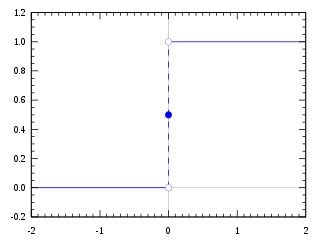
\includegraphics[width=0.5\textwidth]{images/heaviside_function.png}
	\caption{Segnale Gradino Unitario $u(t)$.}
\end{figure}
Tale funzione, discontinua nell'origine, consente una rappresentazione concisa
dei cosiddetti segnali \textit{causali}\footnote{Un segnale causale \`e una
funzione dipendente dal tempo che rappresenta uno stimolo esterno su un sistema
fisico. Matematicamente, un segnale causale \`e rappresentato mediante una
funzione nulla per $t < 0$. L'istante $t = 0$ rappresenta il momento in cui
viene applicato dall'esterno il segnale.} o \textit{cisoidali}, cio\`e
\textit{nulli} per $t < 0$. Si noti che, mentre per $t > 0$ $u(t)$ assume un
valore unitario, nell'origine assume il valore $1/2$.
\bigbreak
Il segnale gradino serve a modellare matematicamente l'accensione all'istante
$t = 0$ di un generatore ideale di tensione continua. che eroga cos\`i una
tensione costante per ogni valore $t \geq 0$. Il  segnale possiede energia
illimitata, in quanto
\begin{equation}
	\begin{split}
		E_u = \int\displaylimits_{-\infty}^{+\infty} \abs{u(t)}^2 \dt =
		\underbrace{\int\displaylimits_{0}^{+\infty} \abs{u(t)}^2 \dt}_{
			u(t) \ = \ 0 \ \forall \ t \ < \ 0}
		= \underbrace{\int\displaylimits_{0}^{+\infty} 1 \dt}_{u(t) \
		= \ 1 \ \forall \ t \ > \ 0} =
		\\
		= \left[ t \right]_0^{+\infty} = +\infty - 0 = +\infty.
		\quads{6}
	\end{split}
\end{equation}
La potenza media $P_u$, invece, \`e espressa dalla relazione
\begin{equation}
	\begin{split}
		P_u = \lim_{T \rightarrow \infty} \frac{1}{T} 
		\int\displaylimits_{-T/2}^{T/2} \abs{u(t)}^2 \dt = 
		\underbrace{\lim_{T \rightarrow \infty} \frac{1}{T} 
		\int\displaylimits_{0}^{T/2} \abs{u(t)}^2 \dt}_{u(t) \ = \ 0 \ 
		\forall \ t \ < \ 0} =
		\\
		= \underbrace{\lim_{T \rightarrow \infty} \frac{1}{T} 
		\int\displaylimits_{0}^{T/2} 1 \dt}_{u(t) \ = \ 1 \ \forall \ 
		t \ > \ 0} = \lim_{T \rightarrow \infty} \frac{1}{T} \left[ t 
		\right]_0^{T/2} =
		\quads{4}
		\\
		= \lim_{T \rightarrow \infty} \frac{1}{T} \left(\frac{T}{2} - 0
		\right) = \lim_{T \rightarrow \infty} \frac{1}{T} \cdot 
		\frac{T}{2} = \frac{1}{2}.
		\quads{4}
	\end{split}
\end{equation}
Il valore efficace \`e dato da
\begin{equation}
	u_{eff} = \sqrt{P_u} = \sqrt{\frac{1}{2}} = \frac{1}{\sqrt{2}},
\end{equation}
mentre il valore medio \`e ottenibile da
\begin{equation}
	\begin{split}
		u_m = \lim_{T \rightarrow \infty} \frac{1}{T} 
		\int\displaylimits_{-T/2}^{T/2} u(t) \dt = \lim_{T \rightarrow 
		\infty} \frac{1}{T} \int\displaylimits_{0}^{T/2} 1 \dt = 
		\lim_{T \rightarrow \infty} \frac{1}{T} \cdot \frac{T}{2} = 
		\frac{1}{2}.
	\end{split}
\end{equation}
\end{document}

